\documentclass[12pt, a4paper]{report}

\usepackage{preamble}     % your custom style file (already uploaded)

\usepackage[round,sort,sectionbib]{natbib}  %  → References heading gets correct size

\usepackage{chapterbib}   % enables a separate .bbl for every \include

% hyperref should come **last**                                    
\usepackage[colorlinks=true,backref=page]{hyperref}
\hypersetup{linkcolor=gray, citecolor=gray, urlcolor=gray}

\title{On Choice, Belief, and Distribution: Axiomatic Studies in Behavioural Economics}
\author{Enrico Mattia Salonia}
\date{16~June~2025}  % or a fixed date

% --------------------------------------------------------------------
\begin{document}
% --------------------------------------------------------------------

% Title page ---------------------------------------------------------
\begin{titlepage}
	\centering
	\makeatletter                   % <— open access to @‑macros
	{\LARGE\bfseries \@title\par}\vspace{2cm}

	%{\Large \textit{A thesis submitted for the degree of Doctor of Philosophy}\par}\vspace{1.5cm}

	%{\Large by\par}\vspace{0.5cm}
	{\Large\bfseries \@author\par}\vspace{0.5cm}  % line 44 — now defined

	{\@date}                        % uses whatever you put in \date{}
	\makeatother                    % <— close @ access
\end{titlepage}


\cleardoublepage

% Roman‑numeral prelims ----------------------------------------------
\pagenumbering{roman}

\cleardoublepage          % or \clearpage   –– finish previous text
\thispagestyle{empty}     % 1. suppress header/footer (hides the number)

% ... any material that belongs on the un-numbered page ...

\vspace*{0.55\textheight}     % tweak this number to move it up/down
\begin{flushright}
	\itshape                   % italic is traditional for a dedication
	To my brothers\par
	with whom I learned to play fair
\end{flushright}


\addtocounter{page}{-1}

\setcounter{page}{2} % title‑page is p. i
\tableofcontents
\cleardoublepage

% Arabic‑numeral main matter -----------------------------------------
\pagenumbering{arabic}
\chapter*{Acknowledgements}\label{ch:ac} % no number
\addcontentsline{toc}{chapter}{Acknowledgements}% put it in the ToC

It would be far too lengthy to acknowledge everyone who contributed to this work, and the many ways they did so. I will therefore name a few people, in no particular order, and mention at least one thing I consider relevant about them, even if it is not necessarily the most important.

I should thank all my friends around the world, but a few special mentions are in order. The first thing Michele told me when we met was that I should never have gone into epistemic game theory; I did my best anyway. Consistently, one of the last things he told me was that a paper in this thesis will probably never be published in a finance journal. To Pau I owe inspiration for a new definition of certainty: an event as likely as finding him in the office when I arrive. My friends from the Caba supported me with words consisting only of one capital letter, but full of meaning. I thank my brothers, to whom this thesis is dedicated, for always playing fair with me even when I lost. I hope we keep learning to play together. I owe gratitude to many professors, but I will mention only a few. François never tired of telling me that my notation was terrible. Interestingly, he once asked about the connection between Bayes rule and mixing liquids. The first time I met Marciano he called one of my ideas a \textquote{bel trucco}. I remain indebted to him for giving me the courage and the support to develop it into a chapter of this thesis. Ingela not only took a bet on me against the odds, she also encouraged me to pursue original ideas and showed me how to nurture them. She praised the long-gone quotations that once opened these chapters—quotes I never had the courage to keep.

Ringrazio i miei genitori, che hanno sempre intravisto per me un futuro da insegnante e ricercatore, sopportando con pazienza i molti alti e bassi del percorso. Mio padre mi ha insegnato a guardare in alto anziché fissare i miei piedi; ho seguito quel consiglio con tale entusiasmo da passare fin troppo tempo a contemplare il cielo. Per fortuna mia madre mi ha sempre ricordato di camminare con i piedi ben dritti. Da loro ho imparato a fantasticare con ordine, un equilibrio ossimorico solo in apparenza che spero si rifletta in questa tesi.

Across continents, for more than a third of my life, and throughout my entire intellectual journey, I have been in Annalisa's loving companionship. We bonded over a shared urge to understand our choices and give them meaning, so much so that it is often hard to tell whether we are discussing research or ourselves. She sees how deeply this thesis reflects my ideas, methods, and aspirations, yet kindly forgives my prose for not matching her eloquence. I thank her for her unique ability to interpret every expression of myself, usually over a good cappuccino in a \textquote{suggestive} spot.
\setcounter{chapter}{0}% <—  important!
\chapter*{Introduction}\label{ch:intro} % no number
\addcontentsline{toc}{chapter}{Introduction}% put it in the ToC

This thesis studies principles underlying individual behaviour, information processing, and resource allocation. It focuses on foundational issues in behavioural economics, where the concepts investigated in this thesis are introduced. Behavioural economics—which examines variations in individual behaviour, belief revision, and normative judgement—has historically been characterized by a reduced-form approach \citep{spieglerBehavioralEconomicsAtheoretical2019}. This approach explains empirical observations through reinterpretations of classical theoretical constructs that intuitively capture relevant psychological mechanisms. In contrast, I argue that more nuanced treatments are necessary, requiring the development of novel theoretical tools rather than merely reinterpreting existing ones. As a result, I derive distinctions within the behavioural phenomena under study that are difficult to discern without explicit modelling.

The chapters appear in the chronological order of their conception. In Chapter \ref{ch:univ}, I study individuals who universalise their behaviour—that is, they consider what would happen if everyone behaved as they do, under different interpretations of this notion. In Chapter \ref{ch:meritocracy}, I examine criteria for the allocation of resources in society that are responsive to considerations of merit and individual responsibility. In Chapter \ref{ch:bdp}, I explore how individuals with preferences over their beliefs behave and interpret new information. Common to all three chapters is the use of the axiomatic method. This approach is natural given the aims of the thesis. In the words of Debreu: \textquote{\textit{Allegiance to rigour dictates the axiomatic form of the analysis where the theory, in the strict sense, is logically entirely disconnected from its interpretations}} \citep[p. x]{debreuTheoryValueAxiomatic1959}. Given the conceptual complexity of the topics at hand, the axiomatic method ensures that the logical development of the theory is not contaminated by its interpretations, leading to \textquote{\textit{a deeper understanding of the problem}} \citep[p. x]{debreuTheoryValueAxiomatic1959}.

In all three chapters, I first introduce a syntax that allows me to describe the objects of interest. The principles under study represent particular instances of these objects. I then specify properties that elements of the syntax must satisfy to be equivalent to the object of interest. In particular, I characterise these objects as the unique elements satisfying the relevant properties. This method is useful because it allows one to express a theory of individual behaviour, belief revision, or resource allocation using a few logically consistent conditions. These conditions serve a dual purpose: first, they can be normatively evaluated—whether they are conditions one might wish to respect when acting, processing information, or distributing goods. Second, they provide testable implications. If an individual’s observed behaviour violates these conditions, then the theory is an inadequate description of that individual’s behaviour. Each chapter includes illustrative applications of the theory in canonical economic settings. I now turn to a brief description of the chapters.

\emph{Chapter \ref{ch:univ}: A Foundation for Universalisation in Games.} The first chapter studies individuals with preferences for universalisation—that is, they consider what would happen if everyone were to act as they do. Universalisation has been shown to have evolutionary foundations, to align with observed behaviour, and to lead to desirable allocations under various normative frameworks. Existing models, such as Homo Moralis preferences \citep{algerHomoMoralisPreference2013} and Kantian equilibrium \citep{roemer2019cooperate}, lack choice-theoretic foundations, limiting their generalisability. To address this, I develop an axiomatic model characterising preferences for universalisation. The main challenge is that universalisation is a non-consequentialist attitude, which is difficult to capture using standard choice-theoretic tools. A key behavioural prediction of my model is that the independence axiom holds only among actions that are universalised in equivalent ways. My framework unifies previous models, introduces a broader class of universalisation preferences, and offers guidance for empirical studies.

\emph{Chapter \ref{ch:meritocracy}: Meritocracy as an End and as a Means.} The second chapter studies the concept of meritocracy, widely discussed both publicly and in the economics and philosophy literature. An allocation is meritocratic if more meritorious individuals obtain more rewarding outcomes. Each instance of meritocracy is characterised by two components: a merit criterion, which determines what counts as meritorious behaviour, and a reward criterion, which specifies which outcomes are more rewarding. By examining whether the allocation choices of impartial spectators align with particular merit and reward criteria, one can test the extent to which individuals adhere to different meritocratic principles. I consider two motivations for supporting meritocracy: rewarding merit as intrinsically fair—interpreting meritocracy as an end—and using meritocracy as an instrument to achieve other goals, such as efficiency—thus treating it as a means. I show that these two justifications are equivalent in terms of the rules they imply. Different assumptions about the merit and reward criteria accommodate various instances of meritocracy. I characterise and examine two meritocratic principles found in the literature: Pareto meritocracy, in which merit derives from generating a Pareto improvement, and proportional meritocracy, in which consumption increases proportionally with effort. I conclude by distinguishing meritocracy from responsibility-sensitive egalitarianism, as in \citep{fleurbaey2008fairness}.

\emph{Chapter \ref{ch:bdp}: Identifying Belief-dependent Preferences.} The third chapter studies individuals whose well-being—their preferences over outcomes—is directly shaped by their beliefs. Such belief-dependent preferences explain a range of behaviours that deviate from expected utility theory. A growing body of evidence suggests that individuals selectively avoid or distort information, consistent with a preference for holding particular beliefs \citep{golmanInformationAvoidance2017}. When beliefs influence preferences over outcomes, belief formation itself may be endogenously shaped by those preferences. This interdependence complicates the task of inferring tastes and beliefs from choice data. The main contribution of the chapter is to present a model of belief-dependent preferences combined with non-Bayesian updating, and to provide choice data sufficient to test and identify the model’s components. I introduce a novel form of choice data, which generalises the notion of a menu in the menu-choice literature, and introduce axioms over preferences on such menus. To clarify the contrast with existing approaches, consider \cite{brunnermeierOptimalExpectations2005}, where individuals choose their beliefs, balancing belief-based utility with material payoffs. While technically equivalent to standard models, this framework departs from prior decision-theoretic foundations by assuming endogenous belief choice. As noted by \cite{eliazCanAnticipatoryFeelings2006} and \cite{spieglerBehavioralEconomicsAtheoretical2019}, this assumption complicates the interpretation and testability of the model. In contrast, my model uses standard tools from choice theory to identify the behavioural implications of belief dependence and provides clear conditions under which the theory can be falsified.

\bibliographystyle{apacite}  % or another  style
\bibliography{references} % .bib file goes in ./bib/
\setcounter{chapter}{0}% <—  important!
\renewcommand{\thefootnote}{\fnsymbol{footnote}}

\chapter[A Foundation for Universalisation in Games]%
        {A Foundation for Universalisation in Games\protect\footnotemark}
\label{ch:univ}

% 2) Put the actual footnote text
\footnotetext{I am indebted to Ingela Alger and François Salanié for countless discussions, comments, and invaluable guidance throughout various stages of this project. I also thank, in random order, Karine Van Der Straeten, Mostapha Diss, Alberto Grillo, Pau Juan Bartroli, Matteo Broso, Annalisa Costella, Philippe De Donder, Giacomo Rubbini, Peter Hammond, Franz Dietrich, two anonymous referees and participants at various workshops and conferences for helpful feedback. I acknowledge funding from the European Research Council (ERC) under the European Union's Horizon 2020 research and innovation programme (grant agreement No 789111 - ERC EvolvingEconomics).}

% 3) Reset things so later footnotes go back to 1, 2, 3, …
\setcounter{footnote}{0}
\renewcommand{\thefootnote}{\arabic{footnote}}


\begin{chapterabstract}
	I study the behaviour of individuals who have preferences for universalisation. When considering a course of action, they evaluate the consequence that would occur if everyone else acted equivalently, according to some criterion of equivalence. That is, they universalise their behaviour. I develop and axiomatise a model for individuals who value their choices in light of the consequences they induce when their action is universalised. The key behavioural prediction is that the independence axiom is satisfied only among actions that are universalised equivalently. I impose conditions to single out the most prominent models of universalisation, compare them, highlight and arguably overcome their limitations. I propose a unifying model of universalisation inspired by the equal sacrifice principle.
\end{chapterabstract}

\section{Introduction}\label{sec:introuniv}

What would I get if everyone acted as I do? An individual who acts based on the answer to this question exhibits universalisation reasoning. In group interactions, universalisation reasoning prescribes that individuals consider what would happen if everyone chooses the same action as them. Universalisation has been shown to have evolutionary foundations \citep{algerHomoMoralisPreference2013} and aligns with behaviour observed in experiments \citep{levineLogicUniversalizationGuides2020,miettinenRevealedPreferencesSequential2020,vanleeuwenEstimatingSocialPreferences2024}. Furthermore, it leads to desirable allocations under several normative criteria \citep{roemerKantianEquilibrium2010}.

Universalisation appears in the literature in various forms, with two prominent formulations being Homo Moralis preferences \citep{algerHomoMoralisPreference2013} and the Kantian equilibrium concept \citep{roemer2019cooperate}. Nevertheless, these models lack choice-theoretic foundations, complicating their unification and empirical testing. Without such foundations, extending the models beyond symmetric settings becomes challenging. It is unclear what \textquote{behaving in the same way} means in asymmetric contexts. Furthermore, the conceptual relationship between universalisation and other pro-social preferences remains unexplored. More worryingly, the models' predictions depend on the labels assigned to the primitive objects of choice, namely, actions in games. Universalisation prescribes considering what happens when everyone chooses the same action, therefore, changing the names of actions alters the predictions of these models. I show that developing choice-theoretic foundations for universalisation allows resolution of these issues.

I develop a model and introduce axioms that characterise preferences for universalisation. This characterisation enables the unification of previous models, rationalises existing empirical identification practices, and provides new testable predictions. I also introduce a new class of preferences for universalisation that are applicable to asymmetric settings. These preferences generalise the symmetric models, and their predictions are independent of the labelling of actions in games.

The main difficulty in modelling universalisation is that it is a non-consequentialist motivation. Preferences over actions do not depend on the material consequences these induce. Therefore, it is not straightforward to identify preferences for universalisation from choices over material consequences.\footnote{\cite{senBehaviourConceptPreference1973} suggested that non-consequentialism poses a challenge for revealed preference theory.} Economics is often resistant to considering non-consequentialist motivations \citep{fleurbaeyEconomicTheoriesJustice2019}. The classical models of \cite{anscombeDefinitionSubjectiveProbability1963} and \cite{savageFoundationsStatistics1972} illustrate this resistance. In these models, individuals rank mappings from uncertain states to consequences, usually referred to as \textquote{acts}. Preferences for an act inducing a sure consequence are equivalent to preferences for that consequence. It is impossible to rank acts according to a criterion that does not depend on their induced consequences without trivializing such a notion, for example, by including the chosen act in the description of consequences. Thus, the question is whether universalisation, as a form of non-consequentialism, can be reconciled with the consequentialist approach of choice theory without resorting to ad hoc solutions.

I show that it is fruitful to study non-consequentialist decision criteria by taking a ranking over actions in a game, not consequences, as the primitive. An example in Section \ref{sec:exampleuniv} illustrates that behaviour consistent with preferences for universalisation in a game cannot be rationalised by a preference ranking over material consequences. This motivates the use of \cite{luce1957games}'s model, where the object of choice is an element of an action set. In a two-player game, an action induces an act, a mapping between the opponent's action and a consequence of the game. The novelty is that preferences over actions are not equivalent to preferences over the induced acts. In particular, the individual cares about the consequence that would obtain if his action is universalised. For instance, in a symmetric game, the individual considers what would happen if his opponent chooses the same action as he does. To capture more general criteria for universalisation, I introduce a universalisation function that maps an individual's action to an opponent's action, given a reference profile of actions. As an example, in Multiplicative Kantian Equilibrium \citep{roemer2019cooperate}, individual actions that deviate from the reference profile by a specific proportion are universalised to opponent's action that deviates by the same proportion.

The main result, Theorem \ref{thm:sep}, provides a representation of preferences over mixed actions. The representation is a convex combination of two components. The first is the usual subjective expected utility. The second is the expected utility over the distribution of consequences obtained if the action is universalised. Therefore, preferences are a generalisation of subjective expected utility. The theorem allows to identify preferences over sure consequences up to the usual affine transformations and beliefs uniquely. The key deviation from expected utility is a violation of the independence axiom. In particular, independence holds only among actions that are universalised equivalently. Such violation of independence also constitutes a novel behavioural prediction. A direct test of a specific model of universalisation requires observing a violation of independence among actions that are universalised equivalently.

Because the theorem is silent on the shape of preferences over sure consequences, it reveals that universalisation and pro-social preferences are distinct assumptions; it is possible for an individual to exhibit both, consistent with empirical evidence \citep{vanleeuwenEstimatingSocialPreferences2024}. Moreover, the theorem implies that welfare analysis for individuals with preferences for universalisation cannot use material consequences as a currency, contrary to the standard practice in Kantian Equilibrium models \citep{roemer2019cooperate}. An individual with consequentialist preferences can always be compensated with material payoff, such as money, to refrain from taking a specific action. This is not true for individuals with preferences for universalisation, as they desire to induce a specific consequence as a result of their action being universalised. Non-consequentialist individuals thus suffer when they cannot choose the action they prefer, regardless of any material compensation. I thus argue that welfare criteria for non-consequentialist preferences may encompass a form of freedom of choice.\footnote{See, for example, \citet[Ch. 10]{fleurbaey2008fairness}.}

By specifying the universalisation function, I provide a choice-theoretic foundation for Homo Moralis preferences for universalisation à la \cite{algerHomoMoralisPreference2013} and the various definitions of Kantian Equilibrium by \cite{roemer2019cooperate}, both of which constitute a generalisation of the model by \cite{laffontMacroeconomicConstraintsEconomic1975}. I comment on the difference between my foundation for Kantian Equilibrium and that of \citeauthor{roemer2019cooperate}. He suggests that his model does not assume preferences that deviate from selfish material satisfaction, but rather a different \textquote{optimisation protocol}. I argue that his model's properties can be preserved by abandoning the distinction between the optimisation protocol and preferences, resulting in a more parsimonious framework in line with classical choice theory.

I develop a novel concept of universalisation inspired by the equal sacrifice principle \citep{mill1885principles,youngDistributiveJusticeTaxation1988}. Consider an individual with any given aim. Given a profile of actions in a game, the individual evaluates a deviation by considering the consequence that would occur if their opponents also deviated to induce an equivalent difference in aim satisfaction, that is, an equal sacrifice. I show that this form of universalisation is equivalent to that of Homo Moralis and Kantian Equilibrium in symmetric games. Moreover, its predictions do not depend on the labelling of actions, nor does its definition require the veil of ignorance construct used to define Homo Moralis in asymmetric contexts.

The paper is organized as follows: In Section \ref{sec:modeluniv}, I introduce the primitives of the model and the axioms. The main theorem is presented in Section \ref{sec:repuniv}. In Section \ref{sec:applicationsuniv}, I show how assumptions on the universalisation function allow me to derive various models of universalisation. Equal sacrifice universalisation is introduced in Section \ref{sec:esu}. Section \ref{sec:conclusionuniv} concludes the paper. A literature review and illustrative example follow.

\textit{Related literature.} In this paper, I study a decision problem as modelled in \cite{luce1957games}. The analysis builds on results by \cite{battigalliMixedExtensionsDecision2017}, who study \citeauthor{luce1957games} decision problems and connect them to the approach in \cite{anscombeDefinitionSubjectiveProbability1963}.

The model here is reminiscent of context-dependent preferences by \cite{gilboaDerivationExpectedUtility2003}. They study collections of individuals' preferences, one for each possible belief, over their actions and an uncertain state. As in this paper, the state is interpreted as opponents' choices. They also start from a primitive ranking over individuals' actions and obtain an expected utility representation in games. However, I here study a subjective beliefs setting, where these are derived from behaviour.

The intuition that non-consequentialist individuals do not care about an act because of its consequences has been highlighted by \cite{chenSocialPreferencesSacred2022}, who develop a choice-theoretic model to guide an experiment testing for the presence of non-consequentialist preferences. They argue that, to identify non-consequentialism from choice, individuals must face the possibility that their actions will not be implemented or observed by the experimenter. Their model has a different interpretation compared to mine. In their experiment, subjects knew that there was a chance that their action would not have been implemented, whereas here there is no such possibility.

The model in this paper allows me to distinguish universalisation from the related concept of magical thinking, studied from a choice-theoretic perspective by \cite{daleyMagicalThinkingRepresentation2017}. An individual exhibits magical thinking if he expects the probability the opponent selects a specific action to increase if he chooses that action. They provide axioms on behaviour in symmetric games that characterize magical thinking. I show that magical thinking and universalisation are different from a choice-theoretic perspective. An individual with preferences for universalisation does not believe he affects opponents' choice.

In this paper, I provide a choice-theoretic foundation for various models of universalisation. The two main alternatives are Homo Moralis preferences by \cite{algerHomoMoralisPreference2013,alger2016evolution,algerEvolutionPreferencesStructured2020} and Kantian Equilibrium by \cite{roemerKantianEquilibrium2010,roemerKantianOptimizationMicrofoundation2015,roemer2019cooperate}. In two-player games, Homo Moralis maximises a convex combination of his payoff and the payoff he would obtain if his opponent behaved as he does. The authors show that, among the set of continuous preferences, Homo Moralis is the only one that is  evolutionary stable for all the game protocols their model covers, when interactions take place under incomplete information, and there is assortativity in the process. The result is generalised to multiplayer games and structured populations by \cite{alger2016evolution} and \cite{algerEvolutionPreferencesStructured2020}. \cite{roemer2019cooperate} introduces a new solution concept, Kantian Equilibrium. He argues that, if individuals are Kantian rather than Nash optimisers, when considering deviating from an action profile they assume other players will deviate in an equivalent manner, where \textquote{equivalent} is defined in various ways. \citeauthor{algerHomoMoralisPreference2013} derive novel preferences from evolutionary analysis and \citeauthor{roemerKantianOptimizationMicrofoundation2015} changes the equilibrium concept, when compared with selfish/Nash individuals. I comment on the relation between these two models in the body of the paper.

This paper relates to studies of universalisation and other non-consequentialist motivations in various settings. Some of these study moral attitudes or their relation with pro-social preferences, as \cite{dewatripontMoralityMarkets2024}, \cite{ellingsenModelSocialDuties2024}, \cite{fleurbaey2023moralmotives} and \cite{laslierUniversalizationAltruism2022}. Others are applications in economic environments, including bargaining \citep{dizarlarKantianEquilibriaClass2023,juan-bartroliMoralPreferencesBargaining2024}, contract theory \citep{sarkisianTeamIncentivesMoral2017,sarkisianOptimalIncentivesSchemes2021,sarkisianScreeningTeamsMoral2021}, public goods \citep{brekkeEconomicModelMoral2003a}, social norms \citep{juan-bartroliInjunctiveNormsTheory2024}, taxation \citep{RePEc:ces:ceswps:_9867}, vaccination \citep{dedonderNashKantGametheoretic2025} and voting \citep{algerHomoMoralisGoes2022,dierksDoesUniversalizationEthics2024,grilloEthicalVotingHeterogenous2022}. Finally, there is interest in choice-theoretic models of individual moral attitudes. For example, \cite{ponthiereEpictetusianRationality2024}, \cite{ponthiere2024stoicism} and \cite{shiEndogenousSocialMinimum2024} study, respectively, Epictetianism, Stoicism and preference for a social minimum consumption level.

\subsection{Illustrative Example}\label{sec:exampleuniv}

I briefly illustrate the contribution of this paper through an example. I show that preferences for universalisation cannot be rationalised by a preference ranking over material consequences, and that predictions of previous models depends on the labeling. I then discuss the solution I propose and how it relates to the existing literature.

Two individuals play the following game. They can go left \( ( \ell ) \), middle \( ( m ) \) or right \( ( r ) \). The numbers in the table are monetary rewards.

\begin{table}[H]
	\begin{center}
		\begin{tabular}{c | c c c}
			\(\mu^{\prime}\) &                     & \(\nicefrac{1}{2}\) & \(\nicefrac{1}{2}\) \\
			\(\mu\)          & \(\nicefrac{1}{2}\) & \(\nicefrac{1}{2}\) &                     \\
			                 & \(\ell\)            & \(m\)               & \(r\)               \\
			\hline
			\(\ell\)         & \(1,1\)             & \(0,0\)             & \(0,0\)             \\
			\(m\)            & \(0,0\)             & \(0,0\)             & \(1,1\)             \\
			\(r\)            & \(0,0\)             & \(1,1\)             & \(0,0\)
		\end{tabular}
	\end{center}
	\caption{Preference reversal.}
	\label{tab:reversal}
\end{table}

Assume the row player has beliefs \(\mu\) in Table \ref{tab:reversal} and thus conjectures his opponent will play \(\ell\) or \(m\), each with probability \(\frac{1}{2}\). By choosing a mixed action, the row player can induce any distribution over consequences that mixes between \((0,0)\) for sure and \((1,1)\) or \((0,0)\) with equal probability. If the row player has preferences for universalisation, he will choose \(\ell\), since it is the action that, if implemented by everyone in this game, maximises his monetary payoff. From a revealed preference perspective, it is inferred that he prefers the lottery \(\frac{1}{2} (1,1 ) + \frac{1}{2} (0,0 )\) to the sure consequence \((0,0 )\). Now, consider a second scenario where the same individual has beliefs \(\mu^{\prime}\) in Table \ref{tab:reversal}, according to which his opponent plays \(m\) or \(r\) with probability \(\frac{1}{2}\). The feasible set of lotteries over consequences is the same as before. Actions \(m\) and \(r\) induce the midpoint between \((0,0 )\) and \((1,1 )\) whereas \(\ell\) induces the sure consequence \((0,0)\). The row player still chooses \(\ell\), as it is again the action that maximises his payoff if implemented by everyone. When \((0,0)\) was available, he revealed to prefer \(\frac{1}{2} (1,1 ) + \frac{1}{2} (0,0 )\). Nevertheless, he exhibits a preference reversal in the second scenario, thus violating the weak axiom of revealed preference. There is no complete and transitive preference relation on lotteries consistent with this choice pattern. This impossibility does not occur for consequentialist preferences defined on distributions of material consequences, such as selfishness, altruism, inequity aversion, or maximin. Therefore, functional forms for preferences for universalisation in the literature represent orderings over objects that are different from distributions over material consequences. This implies that preferences over material consequences should not be the relevant measure for welfare analysis of an individual exhibiting universalisation reasoning, contrary to what \cite{roemer2019cooperate} proposes.

This example also shows that the predictions of models of universalisation depend on the labelling of actions. To avoid the preference reversal, it would suffice to swap the labels of one individual's actions, changing \( m \) to \( r \) and vice versa. Indeed, \cite{roemer2019cooperate} discusses in multiple instances how to change the label of actions to define and employ universalisation. In Section \ref{sec:esu}, I present a novel definition of universalisation, relying on the general theory, that is equivalent under any redescription of actions.

\section{Model}\label{sec:modeluniv}

In this section, I introduce the primitives of the model and the axioms I consider. For any set \( Y \), I denote with \( \Delta ( Y ) \) the set of finite probability distributions over \( Y \).

\paragraph{Primitives.} I focus on two-player games, defined as follows.

\begin{definition}\label{def:game}
	A \textbf{two-player game} is a list \( G = ( \{1,2 \}, ( A_i, \succsim_i )_{i \in \{1,2 \}}, X,  \rho ) \), featuring:\footnote{The textbook by \cite{bonanno2018gametheory} discusses games whose primitives are ordinal preferences.}
	\begin{itemize}
		\item a finite set of actions \(A_i\) for each player \( i \);
		\item a common set of consequences \( X \);
		\item a consequence function \(\rho \colon A_i \times  A_{-i} \rightarrow X \);
		\item player \(i\)'s preferences over mixed actions \(\succsim_i \), for each player \( i \).
	\end{itemize}
\end{definition}

Each pair of pure actions \( (a_i, a_{-i} ) \) induces a consequences \( x = \rho_{a_i, a_{-i}} \) where \( x \in X \). Any mixed action \( \alpha_i \in \Delta ( A_i ) \) induces an \citeauthor{anscombeDefinitionSubjectiveProbability1963} act denoted with \( \rho_{\alpha_i} \colon A_{-i} \rightarrow \Delta ( X ) \) leading to consequence \( x \) under opponent's action \( a_{-i} \) with probability \( \rho_{\alpha_i,a_{-i}} ( x ) = \alpha_i ( \{ a_i \in A_i \: | \: \rho_{a_i,a_{-i}} = x \} ) \). Each pair of mixed actions \( (\alpha_i, \alpha_{-i}) \) induce a distribution over consequence, i.e., the constant act \( \rho_{\alpha_i, \alpha_{-i}} \in \Delta (X) \). I say that a mixed action \( \alpha_i \) induces a constant act if \( \rho_{\alpha_i, a_{-i}} (x) = \rho_{\alpha_i, a^{\prime}_{-i}} (x) \) for each pair \(a_{-i}, a^{\prime}_{-i} \) and \( x \). I assume there exist mixed actions that, under various opponent's actions, can induce every possible distribution of consequences. A sufficient condition for this to hold is that for each consequence \( x \) there exists an action \( a_i \) such that \( \rho_{a_i,a_{-i}} = x \) for each opponent's action \( a_{-i} \). I need such richness assumption to identify preferences, as usual in decision theory. However, in examples of games in this paper, usually only a subset of \( A_i \) of feasible actions is available.\footnote{See \citet[p. 631]{dekelEpistemicGameTheory2015} and references therein for a discussion on elicitation of preferences from bets in games.}

I now introduce a primitive instrumental to capture universalisation reasoning. The idea of universalisation is that, when individual \( i \) is evaluating mixed action \( \alpha_{i} \), he considers the distribution over consequences that would occur if his opponent plays equivalently, under some notion of equivalence. As an example, when the game is symmetric and the action set is the same for both players, he might consider the distribution of consequences induced when his opponent also plays \( \alpha_{i} \). Fix a reference mixed action profile \( ( \alpha^{*}_{i}, \alpha_{-i}^{*} ) \). A universalisation function \( T_{( \alpha^{*}_{i}, \alpha_{-i}^{*} )} \colon \Delta (A_{i} ) \rightarrow \Delta (A_{-i} ) \), maps individual \( i \)'s mixed action to an opponent's mixed action, given a reference profile. For each mixed action \( \alpha_i \), the corresponding \( -i \) universalised action is \( T_{\alpha^{*}_i, \alpha^{*}_{-i}} [\alpha_i] \).

Consider two pure actions inducing the same act. If the individual is consequentialist, he should be indifferent between these two actions, as they induce the same consequences under each opponent's action. Under consequentialism, it would be without loss of generality to study a game in which two actions inducing the same act are identified as the same action. However, preferences for universalisation are not consequentialist, they cannot be reduced to preferences over acts. Therefore, I impose a different notion of equivalence between actions.

I refer to two actions \(a_i\) and \(a_i^{\prime}\) as realisation equivalent if

\[ \left(\rho_{a_i}, \rho_{a_i,T_{\alpha^{*}_i, \alpha^{*}_{-i}} [a_i]}\right) = \left(\rho_{a_i^{\prime}}, \rho_{a_i^{\prime},T_{\alpha^{*}_i, \alpha^{*}_{-i}} [a_i^{\prime}]}\right) .\]

Namely, two actions are realisation equivalent when they induce the same act and the same distribution over consequences when they are universalised. Consider an individual who cares only about the act he induces and the constant act induced under universalisation reasoning. Then, he would be indifferent between two realisation equivalent actions. A game is \textbf{reduced} if realisation equivalent actions are the same action.

I study preferences over mixed actions \( \succsim_i \) of a generic individual \( i \). I introduce axioms on \( \succsim_i \) that characterise the following functional representation.

\begin{definition}\label{def:up}
	A ranking \( \succsim_i \) is a \textbf{Universalisation Preference} (\textit{UP}) with respect to the universalisation function \( T_{\alpha^{*}_i, \alpha^{*}_{-i}}\) if it is represented by

	\begin{equation}\label{eq:up}
		\begin{aligned}
			U_i(\alpha_i) = {} & (1-\kappa) \sum_{a_i, a_{-i}} \alpha_i(a_i) \mu_{i}(a_{-i}) u_i(\rho_{a_i, a_{-i}})                                       \\[1mm]
			{}                 & + \kappa \sum_{a_i, a_{-i}} \alpha_i(a_i) T_{\alpha^{*}_i, \alpha^{*}_{-i}}[ \alpha_i ](a_{-i}) u_i(\rho_{a_i, a_{-i}}) ,
		\end{aligned}
	\end{equation}

	for some utility function \(u_i \colon X \rightarrow \mathbb{R}\) and belief \(\mu_i \in \Delta (A_{-i} )\).
\end{definition}

A \textit{UP} is a linear combination of two components. The first component, weighted by \( 1- \kappa \), is a standard subjective expected utility. The individual computes the probability the action profile \( ( a_i, a_{-i} ) \) realises, which depends on his mixed action \( \alpha_i \) and his belief over opponent's actions \( \mu_{-i} \). Then, he evaluates the consequence \( \rho_{a_i, a_{-i}} \) obtained according to the utility \( u_i \). The second component, weighted by \( \kappa \), is the result of universalisation reasoning. Instead of evaluating the probability an opponent's action realises according to the belief \( \mu_i \), the individual considers the opponent's mixed action that results from universalising his action via the universalisation function \( T_{\alpha^{*}_i, \alpha^{*}_{-i}} \). As an example, when the game is symmetric, and then \( A_i = A_{-i} \), one can define the identity universalisation function as \( T_{\alpha^{*}_i, \alpha^{*}_{-i}} [ \alpha_i ] = \alpha_i \) for each \( \alpha_i \), regardless of the reference profile. I show in Section \ref{sec:applicationsuniv} that the identity universalisation function singles out Homo Moralis preferences from Equation \eqref{eq:up}.

\paragraph{Axioms.} I now introduce the axioms that characterise \textit{UP}. I start with standard axioms allowing me to obtain a utility representation of preferences over mixed actions.

\begin{axiom}\label{ax:wo}
	\labelname{axn:wo}{Weak order} (\textbf{Weak order}) Preferences \(\succsim_i\) are a continuous weak order.
\end{axiom}

\begin{axiom}\label{ax:nond}
	\labelname{axn:nond}{Non-triviality}
	(\textbf{Non-triviality}) There exist \( \alpha_i, \alpha^{\prime}_i \) such that \( \alpha_i \succ \alpha^{\prime}_i \).
\end{axiom}

I now proceed with axioms that characterise preferences for universalisation. First, the individual only satisfies independence among actions that are universalised equivalently. The intuition is as follows. If the individual was a consequentialist, he would satisfy independence, which would result in the standard independence condition among acts. However, the individual is also interested in the distribution of consequences induced when his action is universalised. A mixture of two actions induce a mixture in their corresponding universalised action. Therefore, when mixing, the distribution over consequences induced by the action and its universalised counterpart is not guaranteed to change linearly. Linearity is guaranteed only if the two actions are universalised equivalently.

\begin{axiom}\label{ax:uind}
	\labelname{axn:uind}{Universalisation Independence}
	(\textbf{Universalisation Independence}) If

	\[
		T_{\alpha^{*}_i, \alpha^{*}_{-i}} [ \alpha_i ] = T_{\alpha^{*}_i, \alpha^{*}_{-i}} [ \alpha^{\prime}_i ] = T_{\alpha^{*}_i, \alpha^{*}_{-i}} [ \alpha_{i}^{\prime \prime} ],
	\]

	then, for all \( \lambda \in (0,1)\),

	\[ \alpha \succsim_i \alpha^{\prime}_i \implies \lambda \alpha_i + (1- \lambda ) \alpha_{i}^{\prime \prime} \succsim_i \lambda \alpha^{\prime}_i + (1- \lambda ) \alpha_{i}^{\prime \prime} .
	\]
\end{axiom}

The next axiom states that, when two actions induce the same act, then their ranking depends on the distribution of consequences they induce when universalised. It restricts attention to preferences over actions that not only depend on the induced act, but also on the distribution of consequences induced by the universalised action.

\begin{axiom}\label{ax:ceval}
	\labelname{axn:ceval}{Universalisation evaluation}
	(\textbf{Universalisation evaluation}) If \( \rho_{\alpha_i} = \rho_{\alpha^{\prime}_{i}} \), then

	\[ \alpha_{i} \succsim_{i} \alpha^{\prime}_{i} \: \text{ if and only if } \: \rho_{\alpha_i, T_{\alpha^{*}_i, \alpha^{*}_{-i}} [ \alpha_i ]} \succsim_i \rho_{\alpha^{\prime}_i, T_{\alpha^{*}_i, \alpha^{*}_{-i}} [ \alpha^{\prime}_i ]} \: . \]
\end{axiom}

Lastly, I assume the individual satisfies independence among actions inducing constant acts. The reason is the following. A constant act induces the same distribution of consequences regardless of the opponent's action. Therefore, regardless of how the action is universalised, the opponent is not able to affect the distribution of consequences. There is therefore no reason to violate independence when considering constant acts.

\begin{axiom}\label{ax:lindep}
	\labelname{axn:lindep}{Lotteries independence} (\textbf{Lotteries independence}) If \( \alpha_i, \alpha^{\prime}_i \) and \( \alpha_{i}^{\prime \prime} \) induce constant acts, then for all \( \lambda \in (0,1) \),

	\[ \alpha \succsim_i \alpha^{\prime}_i \implies \lambda \alpha_i + ( 1- \lambda ) \alpha_{i}^{\prime \prime} \succsim_i \lambda \alpha^{\prime}_i + ( 1- \lambda ) \alpha_{i}^{\prime \prime} .\]
\end{axiom}

As an alternative, one could dispense from \usename{axn:lindep} and assume that all actions inducing constant acts are universalised equivalently. Then, \usename{axn:uind} would imply \usename{axn:lindep}. The next section studies the implication of imposing these axioms on preferences over mixed actions.

\section{Functional Representation}\label{sec:repuniv}

The main result of this paper shows that the axioms in the previous section are necessary and sufficient to characterise \textit{UP}.\footnote{All proofs are in Appendix \ref{app:proofsuniv}.}

\begin{theorem}\label{thm:sep}
	A ranking \( \succsim_i \) satisfies \usename{axn:wo}, \usename{axn:nond}, \usename{axn:uind}, \usename{axn:ceval} and \usename{axn:lindep} in a reduced game if and only if it is a \textit{UP}. Moreover, the utility function \( u_i \) is unique up to positive affine transformations and beliefs \( \mu_i \) are unique.
\end{theorem}

Theorem \ref{thm:sep} states that choices of mixed actions satisfying the axioms are consistent with the following utility function: when choosing the mixed action \( \alpha_i \), the individual evaluates the probability that each opponent's action \( a_{-i} \) realises according to his subjective belief \( \mu_i \). However, he also considers the distribution of consequences induced by his mixed action \( \alpha_i \) and the universalised action according to the universalisation function \( T_{\alpha^{*}_i, \alpha^{*}_{-i}} \). The two components are aggregated linearly.

I do not derive the form of \( u_i \), the individual may have any preferences over consequences. This fact clarifies the difference between my exercise and, as an example, that of \cite{rohdePreferenceFoundationFehr2010}. \cite{rohdePreferenceFoundationFehr2010} establishes conditions on a ranking over collective monetary rewards that characterise inequity aversion. In the language of the present paper, she studies the shape of \( u_i \). The axioms here imply nothing about such shape. The representation allows the individual, as an example, to both exhibit preferences for universalisation and, say, inequity aversion, as captured by \( u_i \). Then, in a game, the individual would choose the action that, if universalised, satisfies his inequity averse preference. Theorem \ref{thm:sep} thus clarifies that pro-social and non-consequentialist preferences are not exclusive. On the contrary, these two can coexist.

Lastly, Theorem \ref{thm:sep} allows marking the difference between universalisation and magical thinking. An individual exhibiting magical thinking believes he affects the opponent's probability to choose an action by choosing it himself. An individual with preferences for universalisation, instead, develops standard subjective beliefs about opponents' actions, and his behaviour does not affect them. Since beliefs are standard, their updating should be consistent with Bayes rule in dynamic settings. The first component of the utility function, representing preferences over the induced act, is standard, and therefore results on Bayesian updating holds.\footnote{See e.g. \cite{epsteinRecursiveMultiplepriors2003,ghirardatoRevisitingSavageConditional2002}.} In the next section, I study different forms of the universalisation function corresponding to particular preferences in the literature.

\section{Preferences for Universalisation}\label{sec:applicationsuniv}

In this section, I study conditions on the universalisation function under which \textit{UP} preferences are equivalent to various notions of universalisation in games. I start with Simple Kantian Equilibrium by \cite{roemer2019cooperate}, to later proceed with Homo Moralis by \cite{algerHomoMoralisPreference2013} and conclude with Multiplicative Kantian Equilibrium by \cite{roemer2019cooperate}. I supplement results with discussions on the interpretation of these concepts and the relation between them.

\subsection{Homo Kantiensis and Simple Kantian equilibrium}

In this section, I restrict attention to games with common action sets, where \(A_1= A_2 =A\). Simple Kantian Equilibrium is defined as follows.

\begin{definition}\label{definition:ske}
	An action profile \( ( \alpha, \alpha ) \) constitutes a \textbf{Simple Kantian Equilibrium} (\textit{SKE}) of a game with common action sets if, for all players \(i\) and actions \(\alpha^{\prime}\)

	\[
		\sum_{a_i, a_{-i}} \alpha (a_i) \alpha (a_{-i}) u_i(\rho_{a_i, a_{-i}}) \geq  \sum_{a_i, a_{-i}} \alpha^{\prime} (a_i) \alpha^{\prime} (a_{-i}) u_i(\rho_{a_i, a_{-i}}) .
	\]
\end{definition}

A symmetric mixed action profile constitutes a \textit{SKE} if it induces the best distribution over consequences over all symmetric mixed action profiles. I show that a \textit{SKE} can be interpreted as a Nash Equilibrium in a game between two players with \textit{Homo Kantiensis} preferences.

\begin{definition}\label{def:hk}
	A ranking \( \succsim_i \) is a \textbf{Homo Kantiensis} (\textit{HK}) preference if it is represented by

	\begin{equation}\label{eq:hk}
		U_i ( \alpha ) = \sum_{a_i, a_{-i}} \alpha (a_i) \alpha (a_{-i}) u_i(\rho_{a_i, a_{-i}}) ,
	\end{equation}

	for some utility function \(u_i \colon X \rightarrow \mathbb{R}\).
\end{definition}

When evaluating any mixed action \( \alpha \), a \textit{HK}, first introduced in \cite{laffontMacroeconomicConstraintsEconomic1975}, only considers the distribution over consequences induced when his opponent chooses \( \alpha \) as well. A \textit{HK} is a particular case of a \textit{UP} preference. If \( \kappa = 1 \) and \( T_{\alpha^{*}_i, \alpha^{*}_{-i}} [ \alpha ] = \alpha \) for each \( \alpha\), then Equation \eqref{eq:up} reduces to Equation \eqref{eq:hk}. In other words, a \textit{HK} satisfies the axioms in Theorem \ref{thm:sep} with respect to the identity universalisation function.

\begin{prop}\label{prop:ske}
	An action profile \( (\alpha, \alpha) \) constitutes a \textit{SKE} in a game with common action sets if and only if it constitutes a Nash Equilibrium between two \textit{HK}.
\end{prop}

Proposition \ref{prop:ske} thus establishes that \textit{SKE} is a Nash Equilibrium in a game between two players with preferences over mixed actions satisfying the axioms in Theorem \ref{thm:sep} with respect to the identity universalisation function. The result allows me to compare the foundation I offer for \textit{SKE} with that of \cite{roemer2019cooperate}. He argues that, contrary to other models in economics, he does not assume exotic preferences, but classical self-regarding attitudes.\footnote{See, among many others, \citet[p. 69]{roemer2019cooperate}.} What he varies, instead, is individuals' \textquote{optimisation protocol}, as he refers to it. He contrasts Nash optimisation with Kantian optimisation. Nash optimisation, he maintains, relies on the counterfactual \textquote{what would happen were I to change my action alone?}. Instead, Kantian optimisation induces the counterfactual \textquote{what would happen were I and all others to deviate equally?} This argument is echoed in the papers employing various declinations of Kantian Equilibrium.\footnote{See the papers in the literature review in Section \ref{sec:introuniv}.}

In the following, I argue that, although appealing, such reasoning cannot be backed up by classical choice theory. I do not take any stance on this point. It is legitimate to employ concepts that diverge from standard theory. Nevertheless, this incompatibility is particularly relevant here, as \citeauthor{roemer2019cooperate} relies on his distinction between preferences and optimisation protocol to derive welfare statements.

\citeauthor{roemer2019cooperate}'s description of the Nash counterfactual refers to the logic employed to check whether an action profile constitutes a Nash Equilibrium. Nevertheless, this is only vaguely related to the foundation of the concept.\footnote{\cite{battigalliGameTheoryAnalysis2023} offer a thorough discussion on the interpretation of Nash Equilibrium.} Outside contexts of long repeated interactions and adaptive dynamics, an action in a Nash Equilibrium profile is played by an individual holding correct conjectures about opponents' behaviour.\footnote{See \cite{perea2012epistemic} or \cite{dekelEpistemicGameTheory2015} and references therein.} However, players cannot perform the Nash counterfactual exercise, because they do not know what opponents will do, and are unable to evaluate the gain obtained from a unilateral deviation. An individual in a game selects the action that he considers the best one according to his beliefs about what his opponents will do. In turn, the definition of \textquote{best} is, in economics, his preference. In choice theory, observed behaviour is interpreted as revealing a preference for an object compared with others available, actions in this case. Optimisation is a mathematical technique employed to compute what the maximal element is given a primitive ranking over the objects of choice, it is not a feature of the individual or of an equilibrium concept. There is no empirical observation able to tell that two individuals have the same preferences but different optimisation protocols. If they choose differently in the same problem, by definition they have different preferences.

I show with Proposition \ref{prop:ske} that there is no need to rely on informal arguments regarding how individuals optimise. Behaviour consistent with \textit{SKE} can be interpreted as Nash Equilibrium behaviour in a game between two \textit{HK}. Therefore, \citeauthor{roemer2019cooperate} is correct in arguing that assuming individuals behave according to \textit{SKE} is different from saying that they are pro-social. Nevertheless, this does not mean that they optimise differently.

The critique above has implications for welfare analysis. \citeauthor{roemer2019cooperate}'s argument according to which, in \textit{SKE}, individuals have selfish preferences over material consequences but the optimisation protocol is different from Nash, generates confusion. As I showed in the motivating example, it is possible that an individual who plays according to \textit{SKE} does not have a complete and transitive preference, and hence a utility representation, over material consequences. I believe the closest reformulation of \citeauthor{roemer2019cooperate}'s point is that one can have preferences for universalisation even if the utility index in Theorem \ref{eq:up} for material consequences \( u_i \) is the same as that for consequences induced by universalised actions, as in \textit{UP} preferences in Equation \eqref{eq:up}. Nevertheless, this equivalence does not imply the individual would be indifferent between receiving a monetary amount and acting to induce it as a consequence of universalisation reasoning. Great care must be devoted to make welfare statements for non-consequentialist preferences over actions. Given that universalisation is a preference over actions, one interesting avenue is to consider that welfare should be evaluated in terms of the freedom the individual has in choosing an action he prefers.\footnote{\cite{laslierFreedomEconomics1998} offer a review of approaches on how to conceptualise freedom in economics.}

Proposition \ref{prop:ske} also offers a novel rationale for using mixed actions. Under expected utility, there is always a pure action in the set of best replies to probabilistic conjectures regarding opponents' behaviour. The Nash equilibrium mixed action of player \( i \) can be interpreted as strategic uncertainty from player \( -i \)'s perspective. Nevertheless, a \textit{HK} who plays a mixed action in a \textit{SKE} profile has no interest in being difficult to be predicted by his opponents. In his best reply set, there may be no pure actions. A rationale for employing mixed actions is therefore the adherence to a non-consequentialist attitude.

\subsection{Homo Moralis}\label{subsec:hm}

In this section, I exploit the representation in Theorem \ref{thm:sep} to derive Homo Moralis preferences as a special case of Equation \eqref{eq:up}. I again restrict attention to games with common action sets, to define Homo Moralis preferences as follows.

\begin{definition}
	A ranking \( \succsim_i \) is a \textbf{Homo Moralis} (HM) preference if it is represented by

	\begin{equation}\label{eq:hm}
		\begin{aligned}
			U_i ( \alpha ) = {} & (1-\kappa )\sum_{a_i, a_{-i}} \alpha (a_i) \mu_{i}(a_{-i}) u_i(\rho_{a_i, a_{-i}}) \\[1mm]
			{}                  & + \kappa \sum_{a_i, a_{-i}} \alpha (a_i) \alpha (a_{-i}) u_i(\rho_{a_i, a_{-i}}),
		\end{aligned}
	\end{equation}

	for some utility function \(u_i \colon X \rightarrow \mathbb{R}\) and belief \(\mu_i \in \Delta (A_{-i} )\).
\end{definition}

A Homo Moralis maximises a convex combination between subjective expected utility and expected payoff when both individuals play his action. Contrary to \textit{SKE}, \textit{HM} is a preference, not a property of action profiles. A \textit{HM} with \( \kappa=1 \) is a \textit{HK} and his preferences are represented by Equation \eqref{eq:hk}. A \textit{HM} is a \textit{UP} where the universalisation function is the identity, as in \textit{HK}. If \( T_{\alpha^{*}_i, \alpha^{*}_{-i}} [ \alpha ] = \alpha \) for each \( \alpha\), then Equation \eqref{eq:up} coincides with Equation \eqref{eq:hm}.

A \textit{HM} is not only interested in the consequence obtained when his action is universalised, but trades off consequentialist and non-consequentialist motives. Since \textit{HM} is partially strategic, he also cares about his opponent's action and thus his beliefs matter. However, contrary to magical thinking, a \textit{HM} exhibits standard beliefs that do not depend on his action. Such distinction rationalises current experimental practices relying on identifying beliefs of individuals with preferences for universalisation \citep{vanleeuwenEstimatingSocialPreferences2024}. Moreover, my analysis offers a new behavioural prediction to test for the presence of \textit{HM}, and therefore also of \textit{HK}: they both violate independence between mixed actions that are not universalised equivalently, according to the identity universalisation function.

Both \textit{SKE} and \textit{HM} are well-defined only in games with common action sets. \cite{algerHomoMoralisPreference2013} suggest a way to employ \textit{HM} preferences in asymmetric games. They propose to consider an incomplete information expansion of the basic game where players are not aware of their role, reminiscent of the veil of ignorance of \cite{harsanyiCardinalWelfareIndividualistic1955} and \cite{rawls1971theory}. Such incomplete information game is a symmetric interaction where a strategy is a map between role and action. Universalisation can then be defined as strategies are common across players. The authors refer to this preference as \textit{Ex-ante Homo Moralis}. Another definition of universalisation in asymmetric games is Multiplicative Kantian Equilibrium by \cite{roemer2019cooperate}. In the next section, I discuss Multiplicative Kantian Equilibrium, postponing observations on \textit{Ex-ante HM} to Section \ref{sec:esu}.

\subsection{Multiplicative Kantian equilibrium}\label{sec:mult}

In this section, I discuss the relationship between Multiplicative Kantian Equilibrium and \textit{UP}.\footnote{An equivalent analysis delivers similar results for Additive Kantian Equilibrium \citep{roemer2019cooperate}.} The solution concept is defined in games where the action space has a linear structure. It is employed when players can choose a number from the real line. For simplicity, I follow the recommendation in \citet[p. 42]{roemer2019cooperate} and consider the mixed extension of two-player two-actions games, though developing a generalisation of Multiplicative Kantian Equilibrium to multiple actions games is not trivial.

I remove the restriction to games with common action sets and assume players only have two pure actions available. For each \( \alpha_i \) and \( r \geq 0 \), I denote with \( r \cdot \alpha_i \) an operation that affects \( \alpha_i \) by the multiplicative factor \( r \) and \( 1 - \alpha_i \) by the complementary weight to obtain a probability distribution on pure actions, that is

\[ r \cdot \alpha_i :=\frac{r \alpha_i }{r \alpha_i +(1-\alpha_i)} \: .\]

\begin{definition}
	An action profile \( (\alpha_i, \alpha_{-i} ) \) constitutes a \textbf{Multiplicative Kantian Equilibrium} (\textit{MKE}) of a game if, for all players \( i \) and real numbers \( r \geq 0 \)

	\[
		\sum_{a_i, a_{-i}} \alpha_{i} (a_i) \alpha_{-i} (a_{-i}) u_i(\rho_{a_i, a_{-i}}) \geq \sum_{a_i, a_{-i}} r \cdot \alpha_{i} (a_i) r \cdot \alpha_{-i} (a_{-i}) u_i(\rho_{a_i, a_{-i}}).
	\]
\end{definition}

A mixed action profile constitutes a \textit{MKE} if it induces the best distribution over consequences when compared with all mixed action profiles that can be obtained by multiplying both actions by \( r \).\footnote{According to this definition, \( (0,0) \) is always a \textit{MKE} if it is available.} The notion is well defined as I am restricting attention to two actions. A multiplicative deviation is equivalent to moving weight from one action to the other.

Paralleling the analysis for \textit{SKE}, I show that \textit{MKE} can be interpreted as a Nash Equilibrium in a game between two individuals with Multiplicative Homo Kantiensis preferences, defined as follows.

\begin{definition}\label{definition:mhk}
	A ranking \( \succsim_i \) is a \textbf{Multiplicative Homo Kantiensis} (\textbf{MHK}) preference relative to the profile \( ( \alpha_{i}, \alpha_{-i} ) \) if it is represented by

	\begin{equation}\label{eq:mhk}
		U_i ( r \cdot \alpha_{i} ) = \sum_{a_i, a_{-i}} r \cdot \alpha_{i} (a_i) r \cdot \alpha_{-i} (a_{-i}) u_i(\rho_{a_i, a_{-i}}) ,
	\end{equation}

	for some utility function \(u_i \colon X \rightarrow \mathbb{R}\).
\end{definition}

The difference between \textit{MHK} and \textit{HK} is how actions are universalised, as illustrated in Figure \ref{fig:deviations}. A \textit{HK} only conceives both players choosing the same action. In two-player symmetric games with two actions, these profiles correspond to the diagonal of the square representing mixed actions. Instead, \textit{MHK} considers actions as multiplicative deviations from a specific profile. Universalised actions lie on the line connecting the origin and the reference profile, i.e., all the pairs in which the ratio between the two actions is preserved. A profile \( ( \alpha_i, \alpha_{-i} ) \) constitutes a \textit{MKE} if it is the preferred one for both players compared with any other on the line joining the origin and \( ( \alpha_i, \alpha_{-i} ) \). If \( ( \alpha_i, \alpha_{-i} ) \) lays on the \(45^{\circ}\) line, the two universalisation criteria are identical. In the next section, I discuss a novel version under which the universalisation criterion is endogenous and depends on the game at hand.

\tikzset{every picture/.style={line width=0.75pt}} %set default line width to 0.75pt

\begin{figure}[H]
	\centering
	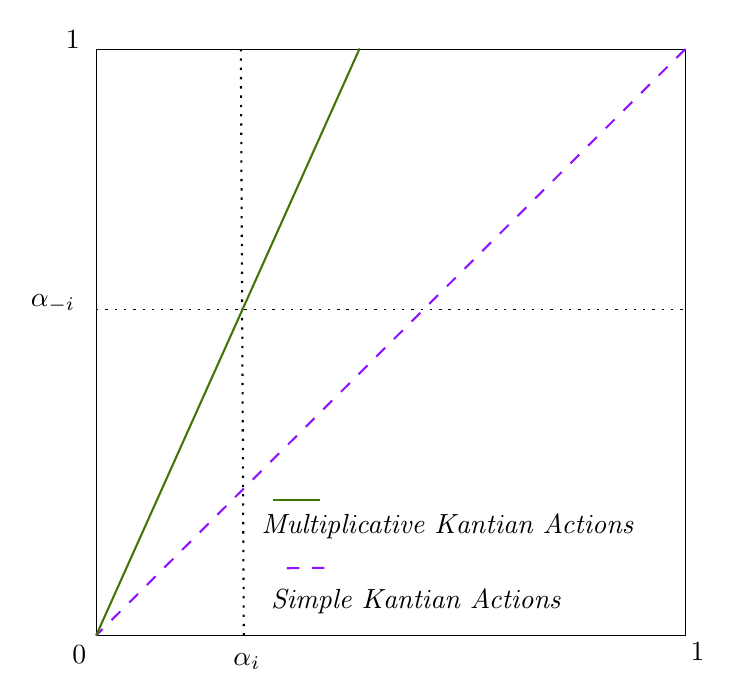
\begin{tikzpicture}[x=0.68pt,y=0.68pt,yscale=-1,xscale=1]
		%uncomment if require: \path (0,474); %set diagram left start at 0, and has height of 474

		%Shape: Rectangle [id:dp48081821398088764] 
		\draw   (141.97,35.82) -- (454.99,35.82) -- (454.99,347.39) -- (141.97,347.39) -- cycle ;
		%Straight Lines [id:da11213906072293889] 
		\draw [color={rgb, 255:red, 144; green, 19; blue, 254 }  ,draw opacity=1 ][line width=0.75]  [dash pattern={on 4.5pt off 4.5pt}]  (454.99,35.82) -- (141.97,347.39) ;
		%Straight Lines [id:da6706664054778095] 
		\draw  [dash pattern={on 0.84pt off 2.51pt}]  (141.97,174.04) -- (454.21,174.04) ;
		%Straight Lines [id:da2856973569143002] 
		\draw [line width=0.75]  [dash pattern={on 0.84pt off 2.51pt}]  (218.85,35.82) -- (220.42,347.39) ;
		%Straight Lines [id:da5420436610131965] 
		\draw [color={rgb, 255:red, 65; green, 117; blue, 5 }  ,draw opacity=1 ][line width=0.75]    (141.97,347.39) -- (282.01,35.43) ;
		%Straight Lines [id:da11662737317060468] 
		\draw [color={rgb, 255:red, 65; green, 117; blue, 5 }  ,draw opacity=1 ][line width=0.75]    (235.88,275.18) -- (260.72,275.18) ;
		%Straight Lines [id:da5716468539586732] 
		\draw [color={rgb, 255:red, 144; green, 19; blue, 254 }  ,draw opacity=1 ][line width=0.75]  [dash pattern={on 4.5pt off 4.5pt}]  (263.22,311.46) -- (239.16,311.72) ;

		% Text Node
		\draw (127.98,351.37) node [anchor=north west][inner sep=0.75pt]    {\( 0 \)};
		% Text Node
		\draw (124.54,24.71) node [anchor=north west][inner sep=0.75pt]    {\( 1 \)};
		% Text Node
		\draw (456.46,349.82) node [anchor=north west][inner sep=0.75pt]    {\( 1 \)};
		% Text Node
		\draw (105.87,164.66) node [anchor=north west][inner sep=0.75pt]    {\( \alpha _{-i} \)};
		% Text Node
		\draw (213.47,355.37) node [anchor=north west][inner sep=0.75pt]    {\( \alpha _{i} \)};
		% Text Node
		\draw (228.54,281.65) node [anchor=north west][inner sep=0.75pt]   [align=left] {\textit{Multiplicative Kantian Actions}};
		% Text Node
		\draw (233.49,321.32) node [anchor=north west][inner sep=0.75pt]   [align=left] {\textit{Simple Kantian Actions}};
	\end{tikzpicture}
	\caption{Universalised action profiles of Simple and Multiplicative Kantian Equilibria.}
	\label{fig:deviations}
\end{figure}

A \textit{MHK} is a particular case of \textit{UP} in which the actions are universalised through a multiplicative logic. If \( \kappa = 1 \) and \( T_{\alpha_i, \alpha_{-i}} [ r \cdot \alpha_i ] = r \cdot \alpha_{-i} \) for each \( r \), then Equation \eqref{eq:up} reduces to Equation \eqref{eq:mhk}.

\begin{prop}\label{prop:mke}
	An action profile \( (\alpha_i, \alpha_{-i}) \) constitutes a \textit{MKE} in a game if and only if it constitutes a Nash Equilibrium between two \textit{MHK} relative to the profile \( ( \alpha_{i}, \alpha_{-i} ) \).
\end{prop}

Proposition \ref{prop:mke} has an interpretation on the lines of its parallel result for \textit{SKE}. It establishes that \textit{MKE} is a Nash Equilibrium in a game between two players with preferences over mixed actions satisfying the axioms in Theorem \ref{thm:sep} with respect to the multiplicative universalisation function. Contrary to \textit{SKE}, \textit{MKE} can be defined when action sets are not common and allows individuals to choose heterogeneous actions, as \textit{Ex-ante HM} does. In the next section, I develop a new concept that takes a different route to define universalisation in games with general action sets.

\section{Equal Sacrifice Universalisation}\label{sec:esu}

In this section, I elaborate on the concept of universalisation and present a new notion, inspired by the equal sacrifice principle \citep{mill1885principles,youngDistributiveJusticeTaxation1988}. The model I propose has several features: its definition does not depend on the label of actions; it can be defined in asymmetric games; in symmetric games it is equivalent to \textit{HM}.

Universalisation requires the definition of two objects. First, it must be transparent what \textquote{doing the same thing} is. Second, it must be equally clear what \textquote{deviating in the same manner} means. For these two concepts to be defined, a common currency must exist for the adjective \textquote{same} to have meaning. Previous ideas employed the label of actions in games and a notion of distance between them when the action space is structured. Such an approach, I argue, is partially lacking. In most economic models, the label of actions bears no conceptual relevance and might be misleading to use it as the main ingredient of a model of universalisation. In fact, in many applications where \textit{MKE} gives intuitive results, the action labels have clear conceptual significance, as they represent effort, contribution to a public good, or use of a common resource.

I propose to use the relevant consequence of the game as a currency. In game theory, this is usually players' utility, but it can be any other index of well-being. Then \textquote{doing the same thing} and \textquote{deviating in the same manner} are interpreted as \textquote{inducing the same utility} and \textquote{inducing the same difference in utility}. The following example illustrates the idea. Consider two individuals playing the prisoners' dilemma. Numbers are Bernoulli utilities for consequences.

\begin{table}[H]
	\begin{center}
		\begin{tabular}{c | c c}
			\(\uglyfrac{\hspace*{0.1cm} 2}{1 \hspace*{0.1cm}}\) & \(a_{2}\) & \(a_{2}^{\prime}\) \\
			\hline
			\(a_{1}\)                                           & \(2,2\)   & \(0,3\)            \\
			\(a_{1}^{\prime}\)                                  & \(3,0\)   & \(1,1\)
		\end{tabular}
		\caption{Prisoners' dilemma.}
	\end{center}
\end{table}

Row player \(1\) attains his highest Bernoulli utility in \((3, 0 )\), induced by the profile \((a^{\prime}_1, a_{2} )\). I define \( \alpha_1^{s} \) as a mixed action which, compared to \( a_1^{\prime} \), given \( a_2 \), induces a reduction in expected Bernoulli utility by \( s \), i.e., \( 3 - [ 2 \alpha_1^{s} + 3 ( 1 - \alpha_1^{s} ) ] = s \). The profile leading to the highest Bernoulli utility for column player \(2\) is instead \((a_1,a_2^{\prime} )\). As for player \(2\), his mixed actions \(\alpha_2^{s}\) induces the difference \( 3 - [ 2 \alpha_2^{s} + 3 ( 1 - \alpha_2^{s} ) ] = s \). Assume that player \(1\), when picking any action \(\alpha_1^{s}\), considers a scenario where \(2\) chooses \(\alpha_2^{s}\). He envisions the consequence that would obtain if his opponent chooses the action that, if considered a unilateral deviation from \((a_1,a_2^{\prime} )\), generates the same difference in Bernoulli utility. In this game, \(\alpha_1^{s} = \alpha_2^{s} = s\) for all \(s\). Whenever they deviate from the action profile that yields their preferred material outcome, both players consider a scenario in which their opponents also deviate by choosing the same action. Therefore, the universalisation is identical to the one of \textit{HK} and \textit{HM} in this example. The actions that lead to the highest Bernoulli utility under this universalisation reasoning are \(a_1\) for \(1\) and \(a_2\) for \(2\), i.e., \( \alpha_1^{s} = \alpha_2^{s} = 1 \), the same optimal actions of \textit{HK} under proper re-labelling of actions.

Evaluating differences from the maximum attainable payoff is reminiscent of the equal sacrifice principle of \cite{mill1885principles} in the context of taxation. Hence, I dub this concept \textit{equal sacrifice universalisation} (\textit{ESU}). An individual with \textit{ESU} preferences first identifies the profile of actions inducing his preferred consequence. Second, he  evaluates each action considering the induced difference in payoff compared with the optimal action computed previously. Third, he individuates the collection of opponents' deviations that, compared with their maximal action profiles in the material dimension, lead to obtain the same absolute difference.

To ease the exposition, I here focus on equal absolute sacrifice \citep{youngDistributiveJusticeTaxation1988}. In Appendix \ref{sec:es}, I consider general equal sacrifice rules. The results and arguments in this section hold for any equal sacrifice rule. Under \usename{axn:wo}, \usename{axn:nond} and \usename{axn:lindep}, preferences over actions inducing constant acts satisfy the standard \citeauthor{anscombeDefinitionSubjectiveProbability1963} conditions. These axioms guarantee the existence of two distributions over consequence \( \overline{\gamma}, \underline{\gamma} \in \Delta (X) \) such that \( \overline{\gamma} \succsim_i \gamma \succsim_i \underline{\gamma} \) for all \( \gamma \). Then, one could define a distribution over consequences inducing sacrifice \( s \) as\footnote{The weight \( \lambda_s \) depends on the normalisation of utility. As an example, if

	\[
		\sum_{x} \overline{\gamma} (x) u_i (x) = S \: \: \text{and} \: \: \sum_{x} \underline{\gamma} (x) u_i (x) = 0,
	\]

	then \( \lambda_s = 1 - \frac{s}{S} \). In fact, by linearity \( \sum_{x} \gamma^s (x) u_i (x) = \lambda_s S \), and I would like that \( \sum_{x} \gamma^s (x) u_i (x) = S - s \), so that

	\[
		\lambda_s S = S - s \: \: \Rightarrow \: \: \lambda_s = 1 - \frac{s}{S} .
	\]}

\[ \gamma^s := \lambda_s \overline{\gamma} + (1- \lambda_s) \underline{\gamma} .\]

Then, define \( \alpha_i^{*}, \alpha_{-i}^{*} \) as any two actions such that \( \rho_{\alpha_i^{*}, \alpha_{-i}^{*}} = \overline{\gamma} \), and \( \alpha_i^s \) as any action such that \( \rho_{\alpha_i^{s}, \alpha_{-i}^{*}} = \gamma^s \). Actions \( \alpha_i^s \) leading to absolute sacrifice \(s\) by definition satisfy

\begin{equation}\label{eq:sacrifice}
	\sum_{a_{-i}} \alpha^{*}_{-i} ( a_{-i} ) \sum_{x} \rho_{\alpha^{*}_i,a_{-i}} ( x ) u_i ( x ) - \sum_{a_{-i}} \alpha^{*}_{-i} ( a_{-i} ) \sum_{x} \rho_{\alpha^{s}_i,a_{-i}} ( x ) u_i ( x ) = s .
\end{equation}

Neither \((\alpha^{*}_i, \alpha^{*}_{-i} )\) nor any \(\alpha_i^s\) are guaranteed to be unique. For the sake of the following definition, I assume they are.\footnote{Therefore, I am implicitly considering a restriction of preferences or games.}

\begin{definition}\label{def:esu}
	A ranking \( \succsim_i \) is an \textbf{Equal Sacrifice Universalisation} preference if it is represented by

	\begin{equation}\label{eq:esu}
		\begin{aligned}
			U_i ( \alpha^{s}_{i} ) = {} & (1-\kappa )\sum_{a_i, a_{-i}} \alpha^{s}_{i} (a_i) \mu_{i}(a_{-i}) u_i(\rho_{a_i, a_{-i}})         \\[1mm]
			{}                          & + \kappa \sum_{a_i, a_{-i}} \alpha^{s}_{i} (a_i) \alpha^{s}_{-i} (a_{-i}) u_i(\rho_{a_i, a_{-i}}),
		\end{aligned}
	\end{equation}

	for some utility function \(u_i \colon X \rightarrow \mathbb{R}\) and belief \(\mu_i \in \Delta (A_{-i} )\).
\end{definition}

When choosing \(\alpha^{s}_i\), the individual evaluates the scenario where his opponent deviates from the action in the profile leading to the highest Bernoulli utility to induce the same sacrifice. \textit{ESU} is a \textit{UP} in which \( T_{\alpha^{*}_i, \alpha^{*}_{-i}} [ \alpha^s_i ] = \alpha_{-i}^s \) for all \( s \), so that Equations \eqref{eq:up} and \eqref{eq:esu} coincide.

The key difference between \textit{ESU} and previous concepts is that universalisation reasoning depends on the game at hand. I illustrate this point in the battle of the sexes. Numbers are again Bernoulli utilities for consequences.

\begin{minipage}[c]{0.3\textwidth}
	\begin{table}[H]
		\begin{center}
			\begin{tabular}{c | c c}
				\(\uglyfrac{\hspace*{0.1cm} 2}{1 \hspace*{0.1cm}}\) & \(a_2\) & \(a_2^{\prime}\) \\
				\hline
				\(a_1\)                                             & \(2,1\) & \(0,0\)          \\
				\(a_1^{\prime}\)                                    & \(0,0\) & \(1,2\)
			\end{tabular}
		\end{center}
		\caption{Asymmetry.}
		\label{tab:asymmetry}
	\end{table}
\end{minipage}
\begin{minipage}[c]{0.3\textwidth}
	\begin{table}[H]
		\begin{center}
			\begin{tabular}{c | c c}
				\(\uglyfrac{\hspace*{0.1cm} 2}{1 \hspace*{0.1cm}}\) & \(a\)   & \(a^{\prime}\) \\
				\hline
				\(a\)                                               & \(2,1\) & \(0,0\)        \\
				\(a^{\prime}\)                                      & \(0,0\) & \(1,2\)
			\end{tabular}
		\end{center}
		\caption{Same Actions.}
		\label{tab:common}
	\end{table}
\end{minipage}
\begin{minipage}[c]{0.3\textwidth}
	\begin{table}[H]
		\begin{center}
			\begin{tabular}{c | c c}
				\(\uglyfrac{\hspace*{0.1cm} 2}{1 \hspace*{0.1cm}}\) & \(a\)   & \(a^{\prime}\) \\
				\hline
				\(a\)                                               & \(0,0\) & \(2,1\)        \\
				\(a^{\prime}\)                                      & \(1,2\) & \(0,0\)
			\end{tabular}
		\end{center}
		\caption{Symmetry.}
		\label{tab:symmetry}
	\end{table}
\end{minipage}

\vspace*{0.4cm}

Consider the game in Table \ref{tab:asymmetry} on the left and assume throughout that \( \kappa = 0 \) for simplicity. The table represents a standard battle of the sexes, in which player \( 1 \) would like to coordinate in the top-left corner, while player \( 2 \) would like to coordinate on the bottom-right corner. The greatest achievable payoff of both players is \(2\), in \((a_1, a_2)\) and \((a_1^{\prime}, a_2^{\prime} )\). The action \(\alpha_1^{s}\) of player \(1\) inducing a sacrifice of \(s\) solves \(2 - 2 \alpha_1^{s} = s\) and hence \(\alpha_1^{s} = \frac{2 - s}{2}\). The equivalent for player \(2\) is \(2 - (2 -  2 \alpha_2^{s}) = s\) which implies \(\alpha_2^{s} = \frac{s}{2} = 1 - \alpha_1^{s}\). The optimum for \textit{ESU} is reached at \(s= \frac{2}{3}\) with \(\alpha_1^{s} = \alpha_2^{s} = \frac{1}{2}\) which, if picked by both players, leads to a common expected payoff of \(\frac{3}{2}\).

This simple example allows me to discuss important differences between \textit{ESU} and previous concepts. First, even if we were to relabel the actions \(( a_2, a_2^{\prime})\) to \((a, a^{\prime} )\) for employing \textit{SKE}, as in the table in the middle, one would not exist anyway. The optimal action is not common, as it is \(a\) for \(1\) and \(a^{\prime}\) for \(2\). Nevertheless, I argue that the problem here is not existence. It is possible to define universalisation from an individual perspective and obtain the profile composed by subjectively optimal actions \(( a, a^{\prime} )\). This is indeed what would happen assuming both players are \textit{HK}. The issue is that it is meaningless to define \textquote{the same thing} as \textquote{the same action} in this scenario. The re-labelling of actions from Table \ref{tab:asymmetry} to \ref{tab:common} is arbitrary as any other, it is not surprising that it does not lead to intuitive results.

As a solution, \citet[p. 26]{roemer2019cooperate} suggests to relabel the game as in Table \ref{tab:symmetry} on the right, to make it symmetric. Now actions are interpreted as \textquote{do the favourite thing} and \textquote{do the least favourite thing}. The \textit{SKE} of this reformulation of the game is \(( \frac{1}{2}, \frac{1}{2} )\), i.e., the optimal actions of \textit{ESU}. Not only the optimal profile coincides, but also the set of profiles considered in the universalisation evaluation is identical. The re-labelling of actions from the first to the third table amounts to changing any mixed action \(\alpha_2^{s}\) to \(1 - \alpha_1^{s}\), which leads to \(a_2=a_1^{\prime}\) and \(a_2^{\prime}=a_1\) and switching columns. This is exactly the \textit{ESU} universalisation reasoning.

Now consider the difference between \textit{ESU} and \textit{Ex-Ante HM}. \textit{Ex-Ante HM} is defined in an incomplete information expansion of the game in which players do not know whether they will be the row player or the column player. When \(\kappa = 1\), it prescribes players to choose the strategy, in this case mapping between identity and action, that ex-ante, before identities are revealed, maximises expected utility over material consequences. The optimal strategies according to such criterion are \((a_1,a_2 )\) and \((a_1^{\prime}, a_2^{\prime} )\). Contrary to what is implemented if both players exhibit \textit{ESU}, these two profiles are Pareto-Efficient. It is already known that \textit{Ex-Ante HM} is related to utilitarian altruism \citep{laslierUniversalizationAltruism2022}. Hence, it is possible that \textit{ESU} delivers an inefficient allocation in terms of material payoff. By contrast, \textit{Ex-ante HM} is always efficient, but is indifferent to inequality.

The following result establishes that optimal actions under \textit{ESU} are always optimal actions under \textit{HK} in symmetric games and therefore the first is a generalisation of the second. The result holds for any equal sacrifice rule, not only absolute sacrifice, as shown in the proof in Appendix \ref{sec:proofs}.

\begin{prop}\label{prop:equivalent}
	Assume the game is symmetric. Then, if an action is optimal under \textit{ESU} with \( \kappa = 1 \), it is also optimal under \textit{HK}.
\end{prop}

The result may be interpreted as a conceptual robustness check. In games where \textquote{same action} has meaning, because of symmetry, \textit{ESU} delivers the intuitive universalisation evaluation of previous concepts. In asymmetric games, the universalisation evaluation depends on the equal sacrifice conception of the individual.

I conclude by addressing possible critiques to \textit{ESU}. First, it relies on interpersonal comparisons of utility, and thus is less parsimonious compared with previous concepts. I acknowledge the issue, but I argue that universalisation always relies on some form of interpersonal comparison and hence the problem is not idiosyncratic to \textit{ESU}. \textit{Ex-ante HM} also relies on the same informational requirement, as it employs the veil of ignorance construct, and thus relies on the same interpersonal comparisons of \citeauthor{harsanyiCardinalUtilityWelfare1953}'s utilitarianism. As for the various forms of Kantian Equilibrium, these rely on interpersonal comparisons of actions, as argued by \cite{sherNormativeAspectsKantian2020}, as actions need to have a cardinal interpretation common to all players. Some form of interpersonal comparisons is therefore needed also in previous conceptions.

The issue is deeper. It is not that universalisation needs some form of interpersonal comparison outside symmetric environments. It always does, but under symmetry, both concepts of \textquote{same action} and \textquote{same utility} have meaning, so comparisons of actions and utility are easy to deal with. Universalisation becomes problematic without symmetry not because of labels, but because of heterogeneity among players. The implicit suggestion of \textit{Ex-ante HM} is to solve such heterogeneity by aggregating preferences in the utilitarian fashion. MKE, instead, suggests to give actions a cardinal meaning. \textit{ESU} offers a third way.\footnote{Incidentally, \textit{ESU} is reminiscent of \cite{kalaiOtherSolutionsNashs1975} bargaining solution.}

A second issue is that \textit{ESU} might lead to corner solutions. The problem is related to the previous one. It is possible that utility indexes across players have different scales and range and this makes it hard for equal sacrifice of utility to be feasible. A partial solution is to perform a proper rescaling of utility.\footnote{Interpersonal comparisons of utility are widely discussed in social choice theory. \citet[Ch. 4]{binmoreGameTheorySocial1994a} and \citet[Ch. 7]{sen2017collective} offer critical overviews of approaches to perform this exercise.} When this is not enough, constrained versions of equal sacrifice, developed by \cite{stovallEqualSacrificeTaxation2020}, can be employed.

\section{Conclusion}\label{sec:conclusionuniv}

I developed and axiomatically characterised a model to account for non-consequentialist preferences for universalisation. The main behavioural prediction is that independence is satisfied only among actions that are universalised equivalently. I showed that the general model unifies the two most prominent models of universalisation, namely Homo Moralis and Kantian Equilibrium. Lastly, inspired by the equal sacrifice principle, I proposed a novel concept of universalisation that does not rely on the labelling of actions, is equivalent to the previous models under symmetry, and can be defined in asymmetric games. I showed how the results shed light on the conceptual underpinnings of universalisation, guide empirical work, and inform the evaluation of welfare statements. In the last paragraphs, I discuss two points regarding the methodology and implications of this paper.

I am not the first to propose changing the set of consequences to account for apparent paradoxes. \cite{baccelliCanRedescriptionsOutcomes2022}, among others, have criticised this practice, as a redescription of the problem might solve technical but not conceptual issues. They argue that it is more reasonable to capture non-material determinants of utility in the evaluation of consequences, without affecting their definition. In this paper, I adhere to this principle. I do not need to alter the set of consequences by including other features in the game. The key is to introduce a link between actions and consequences without changing these two primitives. As my introductory example shows, universalisation cannot be rationalised without assuming that the individual cares about something unrelated to the material consequences of the game. An expansion of the consequence domain is necessary. A second possibility is to include the chosen action in the description of the consequence. It would then be easy to formalise a trade-off between selecting the preferred action and maximising material payoff. This has been done in empirical work on moral preferences, notably by \cite{cappelenPluralismFairnessIdeals2007}. By contrast, my universalisation theory does not rely on assuming that an action is optimal but explains why, i.e., because it induces the preferred universalised consequence.

The final point concerns the nature of preferences for universalisation. I have denoted these as non-consequentialist, and the literature refers to them as moral. Nevertheless, I show that universalisation satisfies consequentialism under an appropriate redefinition of consequences which consider what is induced by the universalised action. What, then, is the difference between universalisation and consequentialist pro-social attitudes? John Broome argues, in \citet[p. 120]{bradleyJohnBroome2021}, that \textquote{\textit{a very specific version of consequentialism is a view I call distribution (it is often called welfarism), which is the view that the goodness of an act is determined by the goodness of the distribution of well-being that results from it}}. Universalisation is, strictly speaking, not a welfarist attitude, as the optimal action is unrelated to the distribution of well-being it induces.

\bibliographystyle{apacite}  % or another  style
\bibliography{references} % .bib file goes in ./bib/

\chapter{Meritocracy as an End and as a Means}\label{ch:meritocracy}

\begin{chapterabstract}
	I introduce a framework for studying different interpretations of meritocracy and testing whether individuals adhere to them. Each meritocracy has two components: a merit criterion, determining when one individual is more meritorious than another, and a reward criterion for each individual, determining when one outcome is more rewarding than another for that individual. An allocation is meritocratic if more meritorious individuals are more rewarded. I distinguish between two conceptions of meritocracy. Meritocracy as an end holds it intrinsically valuable that individuals are rewarded according to their merit. Meritocracy as a means views rewarding merit as instrumental in achieving desirable outcomes according to other standards, such as efficiency. I show that these two conceptions are equivalent: each instance of meritocracy as a means can be associated with a corresponding meritocracy as an end. Finally, I examine two specific meritocracies present in the literature. Pareto meritocracy defines an action as more meritorious if it leads to a Pareto improvement in welfare, whereas proportional meritocracy requires that an individual’s consumption be proportional to the amount of labour he provides. By observing whether allocation choices of impartial spectators align with specific merit criteria, one can test whether spectators adhere to these meritocracies.
\end{chapterabstract}

\section{Introduction}\label{sec:intromerit}

Meritocracy has recently attracted considerable attention in economics and political philosophy \citep{markovitsMeritocracyTrap2019,mulliganJusticeMeritocraticState2018,sandelTyrannyMeritWhat2020, tiroleMeritocracySocialJustice2022}. However, as \citet[p. 5]{senMeritJustice2000} observes, \textquote{\emph{the idea of meritocracy may have many virtues, but clarity is not one of them.}} This paper attempts to bring some clarity. I introduce a framework that allows me to explicitly distinguish between multiple interpretations of meritocracy across different literatures and clarify their relationships. To showcase the use of the framework, I characterise, through assumptions on primitive elements, a particular form of meritocracy referenced in behavioural and experimental economics: proportional meritocracy, according to which an individual's consumption should be proportional to his provided labour.

The setting is as follows. Individuals have preferences over a set of outcomes. A social choice function maps each preference profile to an outcome. A social choice function is meritocratic if it assigns more rewarding outcomes to more meritorious individuals. To express this condition, I consider two criteria: first, the conditions under which an individual or an action is deemed more meritorious; and second, when an outcome qualifies as more rewarding. Accordingly, the framework relies on two fundamental primitives: the \textbf{merit criterion} and the \textbf{reward criterion}. The merit criterion is a binary relation over preferences determining when a preference is more meritorious than another. By interpreting preferences as representations of individual choices, the merit criterion identifies who is more meritorious based on their behavioural attitudes. For example, one might be deemed more meritorious if he requires less consumption as compensation for performing more productive work or if he is more prosocial. The reward criterion for an individual is a binary relation over outcomes determining when an outcome is more rewarding than another for that individual. For instance, an individual may consider an outcome more rewarding if it is preferred to another, it entails more consumption, or it confers public recognition, such as the award of a medal.

I refer to the notion of meritocracy represented by a meritocratic social choice function as \textbf{meritocracy as an end}. One might desire a social choice function to be meritocratic \emph{per se}, independently of any other properties it has. That is, it may be considered intrinsically valuable that an individual is more rewarded if he is more meritorious. This view aligns with desert-based theories of justice in the philosophical literature: \textquote{\emph{It is a good thing, morally speaking, if people are getting what they deserve}} \citep[p. 5]{kaganGeometryDesert2014}.

I also consider a second notion, \textbf{meritocracy as a means}, in which meritocracy is a tool to achieve outcomes desirable according to other criteria. For example, meritocracy as a means could be employed to induce efficient outcomes: \textquote{\emph{the creed of meritocracy: the belief that in the rat race of life rewards should go to the best performers, thereby unleashing society’s full potential}} \citep[p. 1]{morganLimitsMeritocracy2022}. To represent meritocracy as a means, I introduce mechanisms, which consist of a collection of action sets, one for each individual, and an outcome function, mapping each action profile to an outcome. Within a mechanism, a merit criterion is a binary relation over action profiles, determining when an individual's action, given the actions of others, is considered more meritorious. The reward criterion for an individual remains a binary relation over outcomes determining when an outcome is more rewarding than another for that individual. A mechanism is meritocratic if, for each individual, more meritorious actions lead to more rewarding outcomes under the respective criteria.

I derive three results. The first result, Proposition \ref{prop:impl}, details the relationship between meritocracy as an end and meritocracy as a means. I characterise the conditions under which a mechanism implements a meritocratic social choice function. This requires that the mechanism is meritocratic relative to an action-based merit criterion that agrees with the merit criterion over preferences, where agreement means that more meritorious preferences induce more meritorious actions in the mechanism. Therefore, each conception of meritocracy as a means has a meritocracy as an end counterpart. This characterization yields two main implications. First, if one commits to a merit criterion over preferences, the merit criterion over actions of a mechanism is meaningless by itself, as its interpretation relies on the mechanism's outcome function. Common merit criteria in the literature and public discourse are binary relations of the type \textquote{exerting more effort is more meritorious}. However, the result indicates that such criteria are meaningless unless explicitly linked to an outcome function clarifying the implications of effort. Second, if one commits to a merit criterion over actions, independent of the outcome function, he must also accept that such ranking is independent from the outcome the meritocratic mechanism induces. However, this viewpoint is in contrast with meritocracy as a means, as the outcome of the mechanism is thus irrelevant. In a nutshell, one is forced to abandon the idea of meritocracy as a means to stick to a merit criterion over actions as a primitive object.

I showcase the use of the framework and the equivalence between meritocracy as an end and as a means by analysing assumptions on merit and reward criteria that lead to two distinct forms of meritocracy. I start by studying a conception of meritocracy in which an individual's action is more meritorious than another if it leads to a Pareto improvement. The second result, Proposition \ref{prop:pareto}, shows that such merit criterion, if not complemented with other assumptions, is vacuous, in the sense that it ranks as more meritorious preferences ranking Pareto improvement higer than Pareto worsening, but nothing more. Since such Pareto ordering is weak, I proceed to study assumptions on the merit criterion leading to a stronger ordering of preferences.

The third and main result of this paper, Proposition \ref{prop:prop}, is a characterisation of a widely referenced version of meritocracy within a more structured environment, a private goods economy. Individuals provide a labour input to produce a consumption output. They have preferences over pairs of labour and consumption allocations. Several settings in which meritocracy is explored in the literature are particular cases of such economy. I characterise a \textbf{proportional meritocracy}, where each individual's consumption is proportional to his labour input. Proportional meritocracy is characterised by two conditions on the merit criterion and one on the reward criterion. First, the merit criterion is monotonic in the labour input, if one works more, he is more meritorious. Second, the merit criterion is scale-invariant, if the labour input of everyone is multiplied by a constant, the ordering of labour input profiles according to the merit criterion does not change. Third, the reward criterion is welfarist, the reward for merit is individual welfare. I then show that the merit criteria over preferences agreeing with the merit criteria of actions in a proportional meritocracy ranks preferences according to the marginal rate of substitution between labour and consumption. I suggest that such criterion over preferences is more fundamental than one over the labour input, as it can be formulated independently from any specific mechanism. The characterisation of proportional meritocracy can guide empirical studies. Observing allocation choices of an impartial spectator, one could test whether individuals adhere to proportional meritocracy by checking whether they abide by the requirements on the merit criterion.\footnote{See e.g. \cite{cappelenFairnessLimitedInformation2024}.} I further discuss how the present paper paves the way for further empirical evidence on meritocracy in Section \ref{subsec:pareto}. A brief literature review follows.

\emph{Related Literature.} This paper contributes to the literature on responsibility-sensitive social choice theory, surveyed by \cite{fleurbaeyFairnessResponsibilityWelfare2008} and \cite{roemerEqualityOpportunityTheory2016}. The literature develops allocation criteria that are sensitive to factors for which individuals are held responsible, with meritocracy being an instance.\footnote{\cite{carrollEqualOpportunityDifferent2025} discusses the distinction between responsibility-sensitive criteria and standard welfarism.} Equality of opportunity is the main focus of this literature. An allocation rule satisfies equality of opportunity if it neutralises the effects of circumstances beyond individuals' control on their outcomes. One example is allowing students access to education regardless of their parents' income. A key element of this literature is the distinction between compensation for unequal circumstances and reward for choices under control of the individual. A relevant insight is that a compensation criterion for unequal circumstances does not specify a rewarding rule for free actions, these two are distinct concepts. In general, fair compensation is logically independent from fair reward \citep{moulinFairDivisionCollective2004}. Both theoretical and empirical work studying meritocracy often neglect such distinction. Compensation for unequal circumstances is frequently considered a necessary condition for meritocracy, but if the latter is interpreted as a reward criterion for choices, there are no links between the two concepts. This results in meritocracy being conflated with equality of opportunity. In this paper, I propose to view meritocracy as an allocation rule that depends on a merit criterion, regardless of individuals' unequal circumstances. Characterising meritocracy separately from equality of opportunity allows for studying the scope of their intersection. Section \ref{sec:eq} further discussed the relationship between meritocracy and equality of opportunity.

The need for a framework to explicitly discuss meritocracy is revealed by the different meanings different authors give to the same word. I briefly review the theoretical and experimental literature on meritocracy to showcase the lack of common language and conceptual overlap with equal opportunity. I also discuss the relation between past literature and the present work in the body of the text. \cite{moissonCooptationMeritocracyVs2024} study co-optation into an organisation. Candidates have a quality and a personal trait, such as race, gender, or taste. A higher quality trait benefits all members of the organisation. A specific personal trait benefits members with the same trait. The organisation is meritocratic if it selects candidates based on quality traits. Therefore, in this paper, meritocracy is rewarding a trait benefiting more individuals. I study a general version of such assumption in Section \ref{subsec:pareto}. The only distinction between the two traits is the preferences individuals have for them. The underlying idea is that only quality should matter because it is the trait that impacts the firm's output, but equality of opportunity is necessary for individuals with the same productivity not to be discriminated against due to their personal traits. However, such distinction between the two traits is outside the model, as candidates do not choose them, and there is no reason to distinguish them except for employers' preferences.

In \cite{morganLimitsMeritocracy2022}, individuals exert effort in a contest and are rewarded according to a ranking of their performance. There is no meritocracy when the ranking is random, while there is full meritocracy when the ranking precisely reflects the amount of effort exerted. Individuals exert effort to win the contest and obtain a prize. The paper focuses on the relationship between the precision of the ranking and the effort exerted. Interpreting meritocracy as a more or less precise ranking of effort is common, but the reason effort should be rewarded and to which extent is not addressed. Interpreting meritocracy as the precision of effort-based rankings effectively collapses the concept into that of equal opportunity, as randomness can be interpreted as a circumstance outside the individual's control. \cite{moisson2024meritocracy} adheres to a similar definition: in his paper, meritocracy is the relative weight given to effort, ability, and unequal circumstances in determining outcomes.

Similar understandings of meritocracy are also present in the experimental literature. In \cite{cappelenMeritPrimacyEffect2023} and related work by the same authors, subjects in an experiment are divided into workers and spectators.\footnote{\cite{cappelenFairUnfairIncome2020,cappelenMeritocraticOriginEgalitarian2022,cappelenFairnessLimitedInformation2024}.} Workers must complete a real effort task, and spectators have to distribute an amount of money among two workers. The experimental variation is the degree to which the outcome of the effort task is due to the workers' effort or randomness introduced by the experimenter. The idea in \cite{cappelenMeritPrimacyEffect2023} is thus similar to \cite{morganLimitsMeritocracy2022}. Meritocracy is defined as rewarding workers increasingly in their effort. \cite{andreShallowMeritocracy2024} studies how circumstances of which individuals are not in control of shape how meritorious others consider them. One individual has to reward others after observing their choices. He shows that rewards are insensitive to unequal circumstances which shape choices. Both \cite{andreShallowMeritocracy2024} and \cite{cappelenFairnessLimitedInformation2024} more or less explicitly refer to proportional meritocracy, which I discuss in Section \ref{subsec:prop}. Moreover, they find empirical evidence that individuals adhere to such a particular form of meritocracy.

This brief review shows that papers mentioning meritocracy interpret it as a criterion for rewarding effort under equal opportunity, adapted to different settings. Surprisingly, in these papers there is often no reference to the relevant literature in social choice theory on the topic. I will further discuss differences between previous papers and this one in the body of the text.

Lastly, this paper draws from the philosophical literature studying desert-based theories of justice, according to which the allocation of goods in society should reflect individuals' deservingness.\footnote{See \cite{arnesonDesertEquality2007,kaganGeometryDesert2014,sep-meritocracy} for recent developments relevant to the current paper.}

\section{Framework}\label{sec:modelmerit}

Let \(I \) be a finite set of individuals. Each individual \( i \) has preferences \( \succsim_i \in \mathcal{R}_i \) over a set \( X \) of outcomes. I introduce two primitives that allow me to define a meritocratic social choice function. First, a binary relation \( M \) over the set of preferences, determining whether a preference is more meritorious than another, the \textbf{merit criterion}. For each individual \( i \), preference \( \succsim_i \) over outcomes is more meritorious than \( \succsim_i^{\prime} \) if \( \succsim_i M \succsim_i^{\prime} \). The relation \( M \) over preferences is common to all individuals.\footnote{In principle, one could consider an individual dependent merit criterion. Assuming \( M \) is common is equivalent to assuming that only information captured in preferences is relevant, and therefore two individuals with the same preferences should be considered equivalently by \( M \). As a byproduct, \( M \) allows to make interpersonal merit comparisons.} Second, a collection of binary relations \( R_{i} \) over outcomes, one for each individual \( i \), determining whether an outcome is more rewarding to individual \( i \) than another, the \textbf{reward criterion}. An outcome \( x \) is more rewarding to individual \( i \) than \( x^{\prime} \) if \( x R_{i} x^{\prime} \). In general, the reward criterion neither coincides with preferences nor needs to be identical across individuals. Allowing heterogeneous reward criteria lets one tailor the outcome to any relevant differences among individuals. As an example, one might want to reward individuals according to their preferences.

Individuals play a game induced by a mechanism \( \mu = ( ( \mathcal{A}_i )_{i \in I}, g ) \), i.e., a collection of action sets, one for each individual \( i \), and an outcome function  \( g \colon \mathcal{A} \rightarrow X \) mapping each action profile to an outcome. To define a meritocratic mechanism, I introduce a merit criterion over action profiles of the mechanism. Consider a collection of binary relations \( A_i \), one for each individual \( i \), such that, fixing a profile of actions \( a_{-i} \) of individuals other than \( i \), action \( a_i \) of individual \( i \) is more meritorious than \( a_i^{\prime} \) if \( ( a_i, a_{-i} ) A_i ( a_i^{\prime}, a_{-i} ) \). The binary relation \( A_i \) is distinct from \( M \), as the first ranks action profiles in a mechanism, while the second ranks preferences. I discuss a notion of agreement between the two merit criteria in Section \ref{sec:agree}.

\begin{example} \label{ex:priv}
	\labelname{ex:private}{Private Goods Economy} (\textbf{Private Goods Economy}) Several papers studying meritocracy \citep{andreShallowMeritocracy2024,cappelenMeritocraticOriginEgalitarian2022,cappelenMeritPrimacyEffect2023,cappelenFairnessLimitedInformation2024,fleurbaeyFairnessResponsibilityWelfare2008} consider particular instances of an economy with two private goods. The production of \( y \) units of consumption requires \( c ( y ) \) units of labour, where the cost function \( c \) is strictly increasing. Each individual \( i \) has preferences \( \succsim_i \) over his labour and consumption allocation represented by the utility function \( u_i ( \ell_i, y_i ) \), which is strictly decreasing in labour \( \ell_i \), strictly increasing in consumption \( y_i \) and differentiable in both its arguments. An allocation  \( ( \ell, y ) \) is feasible if the total labour input suffices to produce the total consumption \( \sum_{i} \ell_i \geq c ( \sum_i y_i ) \). A social choice function maps each preference profile to a feasible allocation.\footnote{More structure would allow me to consider different productivities. Say that \( \ell_i = b_i e_i \) measures unit of effective labour, where \( b_i \) is productivity. Then preferences are on pairs of \( ( \nicefrac{\ell_i}{b_i}, y_i ) = ( e_i, y_i ) \).} Individuals play the game induced by a mechanism in which their action is the amount of labour they provide \( \ell_i \), and the outcome function maps each labour supply profile to a consumption allocation.

	Denote the marginal rate of substitution between labour and consumption for individual \( i \) in each point by \( \operatorname{MRS}_{\succsim_i} ( \ell_i, y_i ) \), measuring how many units of consumption the individual needs to be compensated for one additional unit of labour. A possible merit criterion states that a preference is more meritorious if, for each level of labour and consumption, it requires less consumption as compensation for one more unit of labour, a version of stakhanovism, that is

	\[ \succsim_i M \succsim_i^{\prime} \quad \Longleftrightarrow \quad \operatorname{MRS}_{\succsim_i} ( \ell_i, y_i ) \leq \operatorname{MRS}_{\succsim_i^{\prime}} ( \ell_i, y_i ) \text{ for each } ( \ell_i, y_i ) \: .\]

	Alternatively, one might consider a merit criterion over actions in the mechanism, according to which a labour supply is more meritorious if it is higher, that is

	\[ ( \ell_i, \ell_{-i} ) A_i ( \ell^{\prime}_i, \ell_{-i} ) \quad \Longleftrightarrow \quad  \ell_i \geq \ell^{\prime}_i \text{ for each } \ell_{-i} \: .\]

	One plausible reward criterion holds that an individual is more rewarded if he receives a preferred allocation, and therefore that \( R_i \) coincides with \( \succsim_i \) for each individual \( i \). Or \( R_i \) might just mean more consumption. I explore the implications of these merit and reward criteria in Section \ref{subsec:prop}. \hfill \( \blacksquare \)
\end{example}

I now discuss the two notions of meritocracy as an end and as a means, starting with the former. A social choice function \( f \colon \mathcal{R} \rightarrow X \) assigns an outcome to each profile of individual preferences. A meritocratic social choice function is defined as follows.

\begin{definition}\label{definition:funcmer}
	A social choice function \( f \) is \textbf{meritocratic} if, for each individual \( i \), for all preferences \( \succsim_i, \succsim_i^{\prime} \) and for each preference profile \( \succsim_{-i} \),

	\[ \succsim_i M \succsim_i^{\prime} \implies f ( \succsim_i, \succsim_{-i} ) R_i f ( \succsim_i^{\prime}, \succsim_{-i} ) \: .\]
\end{definition}

A social choice function is meritocratic if it rewards more, according to the reward criterion, more meritorious preferences, according to the merit criterion. Therefore, different notions of meritocracy correspond to different pairs of criteria. In the words of \cite{senMeritJustice2000}: \textquote{\emph{the notion of merit is fundamentally derivative, and thus cannot but be qualified and contingent}.} Strictly speaking, one should say \textquote{meritocratic with respect to these merit and reward criteria}, but I avoid the qualification when no confusion should arise. Arguably, such modelling choice is convenient as it allows one to trace the underlying sources of disagreement about meritocracy. As an example, some criticise meritocracy because it does not take into account unequal circumstances outside individuals' control. I argue that such a critique could be phrased as disagreement about what the merit criterion \( M \) should trace. One might want it to be independent of features individuals cannot control. Definition \ref{definition:funcmer} represents \textbf{meritocracy as an end}. One might desire the social choice function to be meritocratic regardless of other properties it has: \textquote{\emph{a just distribution is merit-based}} \citep[p. 2]{sep-meritocracy}.

This notion of meritocracy as an end aligns with desert-based theories of justice as studied in \cite{kaganGeometryDesert2014}. The difference is that, in the present setting, I only consider qualitative notions of merit and reward. \cite{kaganGeometryDesert2014} instead assumes that these two are measurable quantities, and is therefore able to describe how far an allocation is from being meritocratic. Definition \ref{definition:funcmer} is instead either satisfied or not. In Section \ref{subsec:prop}, where I introduce proportional meritocracy, I show how assumptions on the merit criterion allow me to derive a quantitative representation of individual merit.

Meritocracy is sometimes conceived as a mechanism for inducing outcomes satisfying other desirable properties, such as Pareto efficient outcomes. To represent such instrumental understanding of meritocracy, I define meritocratic mechanisms.

\begin{definition}\label{definition:mecmer}
	A mechanism \( \mu \) is \textbf{meritocratic} if, for each individual \( i \), for all actions \( a_i, a_i^{\prime} \) and for each action profile \( a_{-i} \),

	\[ ( a_i, a_{-i} ) A_i ( a^{\prime}_i, a_{-i} ) \implies g ( a_i, a_{-i} ) R_i g ( a^{\prime}_i, a_{-i} ) .\]
\end{definition}

A mechanism is meritocratic if it assigns a higher reward as a consequence of an individual choosing a more meritorious action. Definition \ref{definition:mecmer} differs from Definition \ref{definition:funcmer} of meritocratic social choice functions, which assigned a higher reward for individuals who are more meritorious according to their preferences. Definition \ref{definition:mecmer} represents \textbf{meritocracy as a means}. One might ask whether a meritocratic mechanism implements a social choice function satisfying desirable properties. As an example, it is often explored in the literature, and discussed in popular debate, whether meritocratic mechanisms implement efficient outcomes. For instance, \cite{moisson2024meritocracy} examines various definitions of \textquote{merit} based on different weightings assigned to talent, effort, and head start in a specific game. The author investigates which weight distributions achieve desirable outcomes, such as maximizing efficiency in preference satisfaction.

In the next section, I study the relationship between meritocracy as an end and meritocracy as a means as in Definitions \ref{definition:funcmer} and \ref{definition:mecmer}.

\section{When Means and End Coincide}\label{sec:agree}

In this section, I characterise the conditions for a mechanism to implement a meritocratic social choice function. I show that the mechanism must be meritocratic according to a merit criterion on actions of the mechanism that agrees with the merit criterion on individuals' preferences. The notion of agreement is the following.

\begin{definition}
	Fix a mechanism \( \mu \). Two merit criteria \( M \) and \( A_i \) \textbf{agree} if,
	\begin{itemize}
		\item for all actions \( a_i, a^{\prime}_{i} \) and action profiles \( a_{-i} \),
		\item for all preferences \( \succsim_i, \succsim_i^{\prime} \) such that \( g ( a_{i}, a_{-i} ) \succsim_i g ( a^{\prime}_{i}, a_{-i} ) \) and \( g ( a^{\prime}_{i}, a_{-i} ) \succsim_i^{\prime} g ( a_{i}, a_{-i} ) \)
	\end{itemize}

	\[ ( a_i, a_{-i} ) A_i ( a^{\prime}_i, a_{-i} ) \iff \succsim_i M \succsim_i^{\prime} \: . \]
\end{definition}

Crucially, agreement between the two merit criteria depends on the outcome function \( g \). That is, fixing action sets and a merit criterion over preferences, two different outcome functions induce two different criteria of merit over actions agreeing with the original criterion over preferences. In fact, if one wants to adhere to a merit criterion that depends on preferences, it is meaningless to assign a merit criterion to actions, as these might be ranked differently by preferences under different outcome functions.

Instead, if one wants to stick to an understanding of merit that is related to a particular interpretation of actions, such as effort or labour, regardless of the outcome function, one should also accept that such ranking is independent from the outcome the meritocratic mechanism induces. However, this is in contrast with the view of meritocracy as a means, as the outcome of the mechanism is irrelevant for defining a merit criterion over actions. Therefore, supporting both meritocracy as a means and an action-based merit criterion leads to logical inconsistency. In fact, I suggest that it would be more transparent to consider a merit criterion over preferences as a primitive object, and then derive the merit criterion over actions agreeing with it. Moreover, as I show in my next result, any meritocratic mechanism has a meritocratic social choice function counterpart. Therefore, adherence to a meritocratic mechanisms is equivalent to adherence to a meritocratic social choice function.

I now define the notion of implementation I consider. With a slight abuse of notation, I denote a strategy of individual \( i \) in a mechanism with \( a_{i} \colon \mathcal{R}_i \rightarrow \mathcal{A}_i \) mapping each preference to an action. I say that a mechanism \( \mu \) implements a social choice function \( f \) if, for each preference profile \( \succsim \), every Nash equilibrium of the game induced by \( \mu \) results in the outcome \( f ( \succsim ) \).\footnote{See, e.g., \citet[p. 913]{mas-colellMicroeconomicTheory1995}.}

\begin{definition}
	A mechanism \( \mu \) \textbf{implements} a social choice function \( f \) if, for each preference profile \( \succsim \), for each Nash equilibrium strategy profile \( a^{*} \), it holds that \( g( a^{*} ( \succsim ) ) = f ( \succsim ) \).
\end{definition}

I now state my first result, a characterisation of the mechanisms implementing meritocratic social choice functions.\footnote{All proofs are in Appendix \ref{sec:proofsmeritocracy}.} In the statement of the proposition, I do not mention agreement between the two reward criteria, which are assumed to coincide.

\begin{prop}\label{prop:impl}
	A mechanism implements a meritocratic social choice function if and only if: it is meritocratic with respect to some merit criteria \( A_i \); for each \( i \), the merit criteria \( A_i \) and \( M \) agree.
\end{prop}

Proposition \ref{prop:impl} shows that, whenever a meritocratic social choice function is implemented by a mechanism, such mechanism must be meritocratic with respect to the same criteria. The result remarks that, once one is committed to meritocracy as an end, the merit criterion on actions depends on the outcome function of the mechanism, and therefore ranking actions by merit independent of the outcome function is unjustified. Such a discussion raises doubts about common criteria of merit of the type \textquote{exerting more effort is more meritorious.} Conversely, every meritocratic mechanism implements a meritocratic social welfare function according to the same criteria. Therefore, every meritocratic mechanism has a social choice function counterpart.

This equivalence is closely related to the \textquote{control principle} \citep{arnesonDesertEquality2007,fleurbaeyFairnessResponsibilityWelfare2008}, which asserts that, under desert-based theories of justice, individuals should be held accountable only for what lies within their power to control. This principle is elusive to capture within the economic revealed preference framework. If an action causally follows from preferences, it seems odd to hold an individual responsible for them. However, within a mechanism, the action an individual ultimately chooses is shaped by the mechanism itself, via the outcome function. This dependence highlights the arbitrariness of assigning merit to actions, as any action may be part of an equilibrium in a suitable mechanism, thereby violating the control principle. I therefore argue that considering merit criteria over preferences, rather than actions, is more appropriate, despite the criticisms that have been raised against such practice.\footnote{\citet[ch. 10]{fleurbaeyFairnessResponsibilityWelfare2008} offers a comprehensive discussion of this point.}

In the next section, I examine two specific notions of meritocracy that have been employed in the literature. These notions, often implicitly, arise within the context of mechanisms. I use Proposition \ref{prop:impl} to identify their corresponding meritocratic social choice functions.

\section{Two Versions of Meritocracy}\label{sec:priv}

This section explores commonly assumed properties of the merit and reward criteria that give rise to distinct meritocracies. In particular, I study what I call a Pareto meritocracy and (labour) proportional meritocracy. In the first, an action is considered more meritorious if it induces a Pareto improvement. In the second, defined in the private goods economy of Example \ref{ex:priv}, the more an individual works, the more meritorious he is.

\subsection{Pareto Meritocracy}\label{subsec:pareto}

Here, I study a merit criterion according to which an action in a mechanism is more meritorious than another if it induces a Pareto improvement in welfare. The definition follows.

\begin{definition}\label{def:pareto}
	\labelname{axn:pareto}{Pareto Merit}
	A merit criterion \( A_i \) satisfies \textbf{Pareto merit} if, for all actions \( a_i, a_i^{\prime} \) and for each action profile \( a_{-i} \),

	\[ ( a_i, a_{-i} ) A_i ( a^{\prime}_i, a_{-i} ) \iff g ( a_i, a_{-i} ) \succsim_j  g ( a^{\prime}_i, a_{-i} ) \: \text{ for all } \: j \: , \]

	\[ ( a_i, a_{-i} ) A_i ( a^{\prime}_i, a_{-i} ) \iff g ( a_i, a_{-i} ) \succ_j  g ( a^{\prime}_i, a_{-i} ) \: \text{ for some } \: j \: .\]
\end{definition}

In words, fixing an opponents' action profile \( a_{-i} \), an action \( a_i \) scores higher in the merit criterion than action \( a^{\prime}_{i} \) if the outcome resulting from \( a_i \) is weakly preferred to the outcome resulting from \( a^{\prime}_{i} \) by all individuals, and it is strictly preferred by at least one individual. This assumption is frequently invoked in the economic literature and popular debate. As an example, \cite{moissonCooptationMeritocracyVs2024} refer to the employment of a candidate with a talent trait that benefits all members of an organisation as meritocratic. In the philosophical literature, it is argued that a meritocratic governance should be in the hands of capable individuals, able to make people better-off \citep{sep-meritocracy}.

In what follows, I show that the Pareto merit criterion is vacuous in that it only identifies individuals who prefer Pareto improvements as more meritorious—an uninformative condition in standard settings.

\begin{prop}\label{prop:pareto}
	Assume that for each preference \( \succsim_i \) there is a unique maximal element \( x^{*} (\succsim_i) \) in \( X \). Fix a mechanism \( \mu \). Merit criteria over preferences \( M \) agreeing with a merit criterion over actions \( A_i \) satisfying \usename{axn:pareto} must satisfy the following:

	\[
		\succsim_i M \succsim_i^{\prime} \iff x^{*} (\succsim_i) \succsim_j x^{*} (\succsim_i^{\prime})  \: \text{ for all } \: j \: ,
	\]

	\[
		\succsim_i M \succsim_i^{\prime} \iff x^{*} (\succsim_i) \succ_j x^{*} (\succsim_i^{\prime})  \: \text{ for some } \: j \: .
	\]
\end{prop}

To evaluate Proposition \ref{prop:pareto}, consider the implications of the \usename{axn:pareto} criterion in the private economy of Example \ref{ex:priv}. In that setting, each individual prefers a Pareto improvement to a Pareto worsening. Therefore, the \usename{axn:pareto} criterion does not rank any individual as more meritorious than another. In other words, all individuals are equally meritorious according to \usename{axn:pareto}. If not supplemented with other assumptions, the \usename{axn:pareto} criterion does not provide any information about the relative merits of individuals.

It is often argued in philosophy that merit is a contextual phenomenon, suggesting that more structured settings are necessary to meaningfully define it. In the next subsection, I consider a second meritocracy, defined in the more structured setting of Example \ref{ex:priv}, which yields more substantive implications.

\subsection{Proportional Meritocracy}\label{subsec:prop}

In this section, I study a meritocratic mechanism in the setting of Example \ref{ex:priv}. Each individual \( i \) chooses his labour supply \( \ell_i \), and the outcome function \( g \) maps each labour input profile to a feasible consumption profile. In this mechanism, a merit criterion is a binary relation over profiles of labour inputs, while each reward criterion is a binary relation over pairs of labour input and consumption. I study conditions on merit and reward criteria that, under the assumption that the mechanism is meritocratic, uniquely characterise a proportional outcome function, where each individual's consumption is proportional to the labour input he provides.

\begin{definition}\label{def:prop}
	\labelname{def:prop}{Proportional Meritocracy}
	A mechanism is a \textbf{Proportional Meritocracy} if, for each individual \( i \), labour input \( \ell_i, \ell^{\prime}_{i} \) and labour input profile \( \ell_{-i} \),\footnote{With a slight abuse of notation, I do not include the allocation of labour inputs \( g \) induces, as each individual is always assigned his chosen \( \ell_i \).}

	\[ g ( \ell_i, \ell_{-i} ) = \alpha_i(\ell) c^{-1}\left(\sum_{j} \ell_j\right) \: ,\]

	where the numbers \( \alpha_i(\ell) \) satisfy the following conditions:
	\begin{enumerate}
		\item sum to a unit \( \sum_{i} \alpha_i(\ell) = 1 \);
		\item are monotonic in labour inputs \( \ell_i \geq \ell_i^{\prime} \implies \alpha_i (\ell_i, \ell_{-i} ) \geq \alpha_i (\ell_i^{\prime}, \ell_{-i} ) \);
		\item are homogeneous of degree zero, \( \alpha_i (\lambda \ell_1, \ldots, \lambda \ell_{|I|} )=\alpha_i (\ell_1, \ldots, \ell_{|I|} ) \) for any \( \lambda>0 \).
	\end{enumerate}

\end{definition}

Allocation rules similar to \usename{def:prop} have been characterised in various settings, but I follow a slightly different conceptual path.\footnote{See the monograph on claim problems by \cite{thomsonHowDivideWhen2019}.} In a proportional meritocracy, the shares \( \alpha_i \) are interpreted as quantitative measures of merit of individual \( i \). The individual consumes a proportion of the total output, and such proportion coincides with his merit, as measured by \( \alpha_i \). There is a relationship between such interpretation of the allocation rule and a claim problem, where proportional allocations are typically defined. The distinction is that, in claim problems, claims are exogenous, while here the labour input is chosen by the individual once the mechanism is specified. Therefore, a proportional meritocracy might be viewed as a novel rationale for implementing proportional allocation rules, one related to desert-based views of justice.

A proportional conception of meritocracy traces back to Aristotle, who proposed that the ratio of merits and rewards should be equal among individuals \citep{sep-meritocracy}. Taken literally, Aristotle's condition characterises proportional meritocracies in the current setting. For each individual \( i \), his merit is \( \alpha_i \), while his reward is his consumption level

\[ \alpha_i c^{-1}\left(\sum_{j} \ell_j\right) , \]

and the ratio between these two quantities is

\[ c^{-1}\left(\sum_{j} \ell_j\right) , \]

equal among individuals. Therefore, Aristotle's condition is satisfied in a \usename{def:prop}.

I now introduce the assumptions characterising \usename{def:prop}. I start by restricting attention to merit criteria according to which a higher labour input is more meritorious, fixing the labour input profile of all other individuals.

\begin{definition}\label{def:mono}
	\labelname{axn:mono}{Conditional Labour Monotonicity}
	A merit criterion \( A_i \) satisfies \textbf{Conditional Labour Monotonicity} if, for each individual \( i \), labour input \( \ell_i, \ell^{\prime}_{i} \) and labour input profile \( \ell_{-i} \),

	\[ \ell_i \geq \ell_i^{\prime} \implies ( \ell_i, \ell_{-i} ) A_i ( \ell^{\prime}_i, \ell_{-i} ) \: .\]
\end{definition}

\usename{axn:mono} states that, fixing a profile of others' labour input \( \ell_{-i} \), a labour input \( \ell_i \) is more meritorious than \( \ell'_i \) if it is higher. Such definition relies on the structured setting, which allows to measure individual actions. Notice that \usename{axn:mono} does not state that if \( \ell_i \) is higher than \( \ell'_i \) then the first is more meritorious, which would be a stronger requirement, as captured in the following definition.

\begin{definition}\label{def:mono'}
	\labelname{axn:mono'}{Labour Monotonicity}
	A merit criterion \( A_i \) satisfies \textbf{Labour Monotonicity} if, for each individual \( i \), labour input \( \ell_i, \ell^{\prime}_{i} \) and labour input profile \( \ell_{-i} \),

	\[ \ell_i \geq \ell_i^{\prime} \iff ( \ell_i, \ell_{-i} ) A_i ( \ell^{\prime}_i, \ell_{-i} ) \: .\]
\end{definition}

\usename{axn:mono'} states that a higher labour input is more meritorious, regardless of what others' do. Under \usename{axn:mono}, how an individual's labour input scores in merit is conditional on what others' do, which is not the case under \usename{axn:mono'}. This distinction is especially relevant under desert-based theories of justice, because \usename{axn:mono} arguably violates the control principle, stating that individuals should be held accountable only for what is in their control. I study the implications of assuming \usename{axn:mono} or \usename{axn:mono'}, and will show that \usename{axn:mono'} implies a quantitative measure of merit, captured by a number \( \alpha_i \), that only depends on the individual action, while \usename{axn:mono} does not.

Next, I consider a condition on merit criteria establishing that, whenever each individual labour input is multiplied by a positive constant, the merit ranking is preserved, as captured by the following definition.

\begin{definition}
	\label{def:scale}
	\labelname{axn:scale}{Scale-Invariance}
	A merit criterion \( A_i \) satisfies \textbf{Scale-Invariance} if, for each individual \( i \), labour input \( \ell_i, \ell^{\prime}_{i} \), labour input profile \( \ell_{-i} \) and \( \lambda > 0 \),

	\[ ( \ell_i, \ell_{-i} ) A_i ( \ell^{\prime}_i, \ell_{-i} ) \implies ( \lambda \ell_i, \lambda \ell_{-i} ) A_i ( \lambda \ell^{\prime}_i, \lambda \ell_{-i} ) \: .\]
\end{definition}

\usename{axn:scale} is a typical requirement to characterise proportional allocation rules. It states that the merit of an individual depends only on the ratio between his and others' labour input, which is preserved when each of them is multiplied by a constant. Other invariance properties—such as additive invariance—might instead support alternative characterizations of meritocracy in which merit is monotonic in labour, but the consumption allocation depends on merit in other ways than proportional.

Lastly, I introduce the only restriction imposed on the reward criterion: Welfarist Reward. Under Welfarist Reward, an outcome constitutes a higher reward for an individual if it is preferred over another outcome.

\begin{definition}\label{def:welfrew}
	\labelname{axn:welfrew}{Welfarist Reward}
	A reward criterion satisfies \textbf{Welfarist Reward} if \( R_i = \succsim_i \).
\end{definition}

It is often argued in philosophy \citep{arnesonDesertEquality2007,kaganGeometryDesert2014} and tacitly assumed in economics that the appropriate reward criterion should be welfare. In other words, if an individual is more meritorious, he should be better off. Assuming that welfare corresponds to preference satisfaction, \usename{axn:welfrew} represents this assumption.

I now characterise proportional meritocracy.

\begin{prop}\label{prop:prop}

	\begin{enumerate}
		\item A meritocratic mechanism is a \usename{def:prop} if and only if \usename{axn:welfrew}, \usename{axn:mono}, and \usename{axn:scale} hold for each \( i \).
		\item Assume \( | I | \geq 3 \). A meritocratic mechanism is a \usename{def:prop} where, for each \( i \),

		      \[ \alpha_i (\ell) = \frac{\ell_i}{\sum_j \ell_j} \: , \]

		      if and only if \usename{axn:welfrew}, \usename{axn:mono'}, and \usename{axn:scale} hold for each \( i \). In this case, the only merit criterion on preferences agreeing with merit criteria on actions satisfies the following
		      \[ \succsim_i M \succsim_i^{\prime} \quad \Longleftrightarrow \quad \operatorname{MRS}_{\succsim_i} ( \ell_i, y_i ) \leq \operatorname{MRS}_{\succsim_i^{\prime}} ( \ell_i, y_i ) \text{ for each } ( \ell_i, y_i ) \: .\]
	\end{enumerate}
\end{prop}

Proposition \ref{prop:prop} establishes that the stated assumptions are equivalent to a quantitative representation of individual merit via \( \alpha_{i} (\ell) \), which depends on the profile of labour input. Each individual’s consumption corresponds to a share of the total output, where this share reflects their relative merit. If \usename{axn:mono} is strengthened to \usename{axn:mono'}, the measure of merit of each individual is just his labour supply, and thus does not depend on others' actions.

The second item of Proposition \ref{prop:prop} establishes that, under \usename{axn:mono'}, the merit criterion on preferences agreeing with the merit criterion on actions is a ranking of marginal rates of substitution between labour and consumption. Such equivalence gives a more fundamental interpretation of the merit criterion underlying \usename{def:prop}. Under different outcome functions, an individual might choose different levels of labour inputs, rendering the interpretation of the merit criterion as a measure of effort less meaningful. Instead, the marginal rate of substitution is independent of the outcome function.

There is empirical evidence suggesting that individuals adhere to a form of \usename{def:prop} \citep{andreShallowMeritocracy2024,cappelenFairnessLimitedInformation2024}. However, these empirical studies primarily test whether impartial observers' choices satisfy \usename{axn:mono'}, without discussing other conditions, such as \usename{axn:mono} or \usename{axn:scale}. Proposition \ref{prop:prop} shows that a test of \usename{axn:mono'} is not enough to conclude one adheres to \usename{def:prop}, and should be complemented with other empirical results. The result hopefully showcases how the framework in this paper could be employed to advance empirical studies of meritocracy. By introducing other assumptions, such as the additive invariance discussed before, other forms of meritocracies could be characterised, and empirical studies could be designed to test whether impartial observers adhere to them.

\section{Meritocracy and Equality of Opportunity}\label{sec:eq}

Before concluding, I briefly examine the relationship between meritocracy, as defined in this paper, and the concept of equality of opportunity, terms that are often used interchangeably in the economic literature. For this purpose, I compare the model here with the responsibility-sensitive allocation model of \cite{fleurbaeyFairnessResponsibilityWelfare2008}. I discuss a simplified version of his general model, which is also a particular case of the private good economy of the previous section. I show that meritocracy, understood as an allocation rule rewarding merit, is distinct from equality of opportunity, i.e., guaranteeing that each individual \textquote{starts on the same line}, a point that has already been made elsewhere \citep{moulinFairDivisionCollective2004,fleurbaeyFairnessResponsibilityWelfare2008}, but is often neglected in more recent literature.

There are four individuals, each of whom has a level of bequest \( b_i \in \{1, 3 \} \) and dedication \( a_i \in \{ 1, 3 \} \), determining their production in monetary amounts. The set of outcomes is the set of monetary allocations such that \( \sum_i x_i = \sum_i b_i a_i \). Each individual \( i \) prefers to have more money. An allocation rule maps bequest and action profiles to monetary allocations. Consider an allocation rule under which each individual consumes what he produces and there are no transfers. Such allocation rule is illustrated in the following table.

\begin{table}[H]
	\caption{No transfers}
	\begin{center}
		\begin{tabular}{ |c|cc| }
			\hline
			\( x_i = b_i a_i \)        & low dedication \( a_i = 1 \) & high dedication \( a_i = 3 \) \\
			\hline
			low bequest \( b_i = 1 \)  & 1                            & 3                             \\
			high bequest \( b_i = 3 \) & 3                            & 9                             \\
			\hline
		\end{tabular}
	\end{center}
\end{table}

Under this allocation rule, individuals with high bequest obtain a better outcome, thus violating equality of opportunity, since bequests are outside their control. The next table illustrates a second allocation rule neutralising the effect of bequests, transferring from individuals with high bequest to individuals with low bequest.

\begin{table}[H]
	\caption{Neutralising bequests}
	\label{tb:eq}
	\begin{center}
		\begin{tabular}{ |c|cc| }
			\hline
			\( x_i = ( b_i + t_i )a_i \) & low dedication \( a_i = 1 \) & high dedication \( a_i = 3 \) \\
			\hline
			low bequest \( b_i = 1 \)    & 2 (transfer = +1)            & 6     (transfer = +1)         \\
			high bequest \( b_i = 3 \)   & 2   (transfer = -1)          & 6    (transfer = -1)          \\
			\hline
		\end{tabular}
	\end{center}
\end{table}

This allocation rule may be described as one satisfying equality of opportunity, as it neutralises the effect of unequal bequests in determining the outcome. However, the allocation rule in Table \ref{tb:eq} is not the only one satisfying equality of opportunity. One might want to reward high dedication, and therefore induce a better outcome for individuals with high dedication. The following table illustrates such an allocation rule.

\begin{table}[H]
	\caption{Neutralising bequests and rewarding dedication}
	\label{tb:eq2}
	\begin{center}
		\begin{tabular}{ |c|cc| }
			\hline
			\( x_i = ( b_i + t_i )a_i \) & low dedication \( a_i = 1 \) & high dedication \( a_i = 3 \) \\
			\hline
			low bequest \( b_i = 1 \)    & 1 (transfer = +0)            & 9     (transfer = +2)         \\
			high bequest \( b_i = 3 \)   & 1   (transfer = -2)          & 9    (transfer = +0)          \\
			\hline
		\end{tabular}
	\end{center}
\end{table}

A third allocation rule which rewards dedication independently of bequests is the following.

\begin{table}[H]
	\caption{Rewarding dedication}
	\label{tb:rew}
	\begin{center}
		\begin{tabular}{ |c|cc| }
			\hline
			\( x_i = ( b_i + t_i )a_i \) & low dedication \( a_i = 1 \) & high dedication \( a_i = 3 \) \\
			\hline
			low bequest \( b_i = 1 \)    & 0 (transfer = -1)            & 6      (transfer = +1)        \\
			high bequest \( b_i = 3 \)   & 2   (transfer = -1)          & 12    (transfer = +1)         \\
			\hline
		\end{tabular}
	\end{center}
\end{table}

Tables \ref{tb:eq} and \ref{tb:eq2} both represent allocation rules consistent with equality of opportunity, though they differ in how they reward dedication. Instead, allocations in Tables \ref{tb:eq2} and \ref{tb:rew} both reward dedication, but the first satisfies equality of opportunity and the second does not.

Since they are logically independent, meritocracy and equality of opportunity can be combined. For instance, in the private good economy of Example \ref{ex:priv}, one could put more structure to distinguish between labour input and productivity of each individual. Then, the merit criterion could be monotonic in labour input, rather than in productive units of labour, under the assumption that productivity comes from sources the individual cannot control, such as bequests. These requirements would complement the meritocratic idea of rewarding more effort and the equality of opportunity idea of neutralising the effect of bequests. Distinguishing these two concepts clarifies the rationale behind various allocation rules, and gives guidance on how to identify the two components separately in experiments, where these ideas are often conflated.\footnote{As an example, \cite{andreShallowMeritocracy2024} defines \textquote{Shallow Meritocracy} as an allocation rule that does not take into account unequal circumstances. I argue that \textquote{Shallow Meritocracy} is more accurately described as a lack of equality of opportunity, rather than a failure of meritocracy.}

\section{Conclusion}\label{sec:conclusionmerit}

This paper develops a unifying framework for analysing meritocracy, distinguishing between two conceptually distinct notions: meritocracy as an end, represented by meritocratic social choice functions, and meritocracy as a means, represented by meritocratic mechanisms. The core innovation lies in introducing two primitives: a merit criterion that identifies when one individual is more meritorious and a reward criterion that determines which outcomes constitute superior rewards. I thus suggest that common disagreements on meritocracy can often be traced to different assumptions about the merit and reward criteria.

I showed that meritocracy as an end and as a means are equivalent, in the sense that a mechanism implementing a meritocratic social choice function is itself meritocratic. Therefore, adhering to a notion of meritocracy as a means is equivalent to adhering to a notion of meritocracy as an end. This equivalence permits merit criteria to be consistently expressed over either individuals’ preferences or their actions within a mechanism.

I examined two illustrative conceptions of meritocracy from the literature: Pareto meritocracy and proportional meritocracy. I showed that Pareto meritocracy is vacuous, as it only ranks individuals who prefer a Pareto improvement to a Pareto worsening. Proportional meritocracy, defined in a private goods economy in which individuals supply labour and share their production, is more structured and allows to define a quantitative measure of merit. Assumptions on the merit and reward criteria characterise a mechanism in which each individual consumes a proportion of the total output, and such proportion coincides with his merit.

The study of meritocracy as an allocation principle remains in its early stages. Given the empirical evidence supporting the conclusion that individuals adhere to various forms of meritocracy, theoretical study is much needed. Future work could explore the implications of alternative meritocracies in other settings, or empirically test whether individuals adhere to specific meritocracies. Additionally, the relationship between meritocracy and other social justice principles, such as equality of opportunity, warrants further investigation.

\bibliographystyle{apacite}  % or another  style
\bibliography{references} % .bib file goes in ./bib/

\chapter{Identifying Belief-Dependent Preferences}\label{ch:bdp}

\begin{chapterabstract}
	Why are investors overconfident and trade excessively? Why do patients at health risk avoid testing? Why are voters polarised? Possibly because their beliefs directly influence their well-being, i.e., they have belief-dependent preferences. However, existing theories of belief-dependent preferences struggle to generate testable predictions or to identify simultaneously beliefs and preferences. This paper addresses these issues by providing an axiomatic characterization of a class of preferences and belief-updating rules that deviate from Bayesian updating. Preferences, beliefs, and updating rules are identified from choices over contingent menus, each entailing a menu of acts available at a later time contingent on an uncertain state of the world. The results provide a theory-based approach to experimental designs to test information avoidance, distortion, and other behaviours consistent with belief-dependent preferences.
\end{chapterabstract}

%\epigraph{\begin{minipage}{\epigraphwidth}\textit{Fanshawe's praise, therefore, left me with mixed feelings. On the one hand, I knew that he was wrong. On the other hand (and this is where it gets murky), I wanted to believe that he was right. I thought: is it possible that I've been too hard on myself? And once I began to think that, I was lost. But who wouldn't jump at the chance to redeem himself—what man is strong enough to reject the possibility of hope? The thought flickered through me that I could one day be resurrected in my own eyes.}\end{minipage}}{\cite{austerNewYorkTrilogy2006}}

%\epigraph{\begin{minipage}{\epigraphwidth}\textit{Fanshawe's praise, therefore, left me with mixed feelings. On the one hand, I knew that he was wrong. On the other hand, I wanted to believe that he was right. I thought: is it possible that I've been too hard on myself? But who wouldn't jump at the chance to redeem himself—what man is strong enough to reject the possibility of hope? The thought flickered through me that I could one day be resurrected in my own eyes.}\end{minipage}}{\cite{austerNewYorkTrilogy2006}}

\section{Introduction}\label{sec:intro}

People often hold some beliefs dear, even when faced with evidence against them. Do they change their views, or do they continue believing what they want? Indeed, research documents two common attitudes towards new information: avoidance and distortion. Investors avoid obtaining information when they expect the market to be in a bad state \citep{karlssonOstrichEffectSelective2009,sichermanFinancialAttention2016}. Donors do not learn about the impact of their donation \citep{andreoniAvoidingAskField2017,chanAvoidingPeerInformation2024}. Voters shun evidence that undermines their view \citep{gentzkowWhatDrivesMedia2010,bakshyExposureIdeologicallyDiverse2015}. Despite being at risk, patients refrain from getting tested. \citep{thorntonDemandImpactLearning2008,osterOptimalExpectationsLimited2013}. If information is obtained, it is distorted when unwelcome but correctly processed if welcomed. Negotiators interpret favourably information that supports their case and dismiss the quality of contrary evidence \citep{babcockBiasedJudgmentsFairness1995}. Individuals are less likely to accept bad news about their attractiveness or intelligence but correctly process good news \citep{eilGoodNewsbadNews2011}. They also exaggerate good news about their ability or IQ \citep{mobiusManagingSelfConfidenceTheory2022,drobnerMotivatedBeliefUpdating2024}. Those with differing opinions on climate change consider scientists experts only when they support their views \citep{kahanPolarizingImpactScience2012}.\footnote{For additional examples of information avoidance and distortion, see the surveys by \cite{danielOverconfidentInvestorsPredictable2015}, \cite{benabou2016mindful}, and \cite{golmanInformationAvoidance2017}.}

These observations conflict with expected utility theory, where more information is always desirable, and information should be processed via Bayes rule. However, if an individual derives pleasure or pain from specific beliefs, she might avoid information or process it differently. Theories of belief-dependent preferences (hereafter BDP) assume that individuals hold beliefs to enhance their well-being, which explains why they might avoid or distort information. Examples include psychological expected utility \citep{caplinPsychologicalExpectedUtility2001}, optimal expectations \citep{brunnermeierOptimalExpectations2005}, ego concerns \citep{koszegiEgoUtilityOverconfidence2006}, preferences for anticipation \citep{koszegiUtilityAnticipationPersonal2010}, and motivated reasoning \citep{benabouEconomicsMotivatedBeliefs2015,benabou2016mindful}. These theories share a common feature: they do not provide observable data to separately identify the individual’s tastes over outcomes and beliefs. This lack of identification complicates the interpretation of empirical findings, renders distinguishing between different theories difficult, and limits policy recommendations. For accurate predictions and effective policy, economists need models that are identifiable and refutable. In this paper, I offer such a model. My model implies conditions on observed choices that exhaustively characterise BDP. If choices abide by these conditions, then tastes and beliefs can be identified separately. If they do not, the theory is rejected. Such "if and only if" characterisation is absent in previous theories.

In theories of BDP, how an outcome is evaluated depends on the individual's beliefs. The lack of separation between these two concepts complicates their interpretation and identification because the way beliefs are formed may depend on tastes. Inferring tastes and beliefs from choices thus becomes a challenging task. The implication is that it is harder to obtain clear predictions. In addition to the lack of identification, current approaches make different assumptions about information processing, ranging from using Bayes rule \citep{koszegiEgoUtilityOverconfidence2006} to assuming that individuals forget information \citep{benabouEconomicsMotivatedBeliefs2015} or even choose their beliefs at will \citep{brunnermeierOptimalExpectations2005}. These assumptions are difficult to test. Therefore, the extant theories of BDP have two related limitations. They fail to make explicit the link between tastes and belief revision and tastes and beliefs are not uniquely identified.

In this paper, I propose a model of BDP that addresses these limitations. I introduce axioms on choices that characterise individuals as having tastes over their beliefs and belief revision rules related to their tastes. The theory identifies prior beliefs, tastes, and their related belief updating rules from observable choices.

I study the preferences over contingent menus. Contingent menus are collections of acts available at a later time that are conditional on the realisation of an uncertain state of the world. Consider the following illustrative example. An investor can access her banking app to receive information about the market. If she accesses the app, she observes information such as prices or the available balance. She then chooses how much to invest or withdraw. Accessing the app or not represent two \textit{contingent menus}, each associated to a probability distribution over menus of available acts. The realisation of the menu of acts that is finally available to the individual is conditional on an uncertain state of the world. Thus, observing an available menu of acts is informative for the investor. For example, if the investor opens the app and observes a high value of her portfolio, she receives information not only about the amount of money she can withdraw but also about the state of the market. If she chooses not to access the app, she receives no information about the market and her only available act is to do nothing.

The choice between contingent menus thus reflects intertemporal preferences over acts and information. As suggested by this illustrative example, in the general model of an individual's decision problem, there are three time periods. The individual first chooses one of the available \textit{contingent menus}, each of which delivers a distribution of menus of acts conditional on the state of the world. Then, a menu of acts available to the individual realises, and the individual updates her beliefs on the basis of the observation of the realised menu. Finally, the individual chooses an act from the realised menu.

The reason why contingent menus allow for identification is as follows. Consider an individual who has to choose between Blackwell experiments. A Bayesian individual always prefers the most informative experiment. Instead, intuitively, individuals with different preferences over beliefs should prefer different experiments. When an individual with BDP chooses between experiments, she takes expectations over her belief-dependent expected utility, particularly over the posteriors that the experiments can induce. Under Bayesian updating, the mean of the posteriors induced by any experiment is equal to the prior. Therefore, if the individual maximises her belief-dependent expected utility under Bayesian updating, her choices over experiments cannot reveal preferences over distinct posteriors, as their expectations are the same. The intuition that different belief-dependent preferences correspond to different choices of experiments fails, as shown by \cite{eliazCanAnticipatoryFeelings2006} and \cite{liangInformationdependentExpectedUtility2017}. An immediate implication is that non-Bayesian updating overcomes this problem, as the mean of posteriors that are not the Bayesian update of a prior is not necessarily equal to the prior. However, non-Bayesian updating induces dynamic inconsistency. Choices over contingent menus allow me to identify how the individual manages such dynamic inconsistency, that is, how she deviates from Bayesian updating. In turn, non-Bayesian updating allows for the identification of preferences over beliefs.

Two crucial axioms characterise BDP preferences over contingent menus. First, I need an axiom similar to the independence of \cite{vonneumannTheoryGamesEconomic2007}, but weakened to obtain BDP. Here individuals are sensitive to the informational content of a realised menu of acts. Therefore, I formulate a weak version of independence that is satisfied only among contingent menus inducing the same inference about the uncertain state \citep{liangInformationdependentExpectedUtility2017,rommeswinkelPreferenceKnowledge2023}. This weak version of independence induces dynamic inconsistency. After receiving information, the individual is tempted to deviate from her plan. This is because, since individual tastes depend on beliefs, the individual might distort them after receiving information. The second axiom states that the individual faces no temptation when the realised menu of acts comprises her preferred choice under both the Bayesian posterior and according to her preferred posterior. This axiom, which I call \textit{strategic rationality for best likelihood}, ascribes the source of temptation to distorted belief updating due to BDP, and constitutes the main departure from the literature. The axiom is intuitive: it implies that the individual is not tempted when the information she receives is the one she prefers.

The main result is Theorem \ref{thm:rep}, which provides a functional representation of preferences over contingent menus. The choices that are consistent with the representation can be interpreted as follows. The individual chooses a contingent menu according to her preferences over acts in menu realisations and over the information it provides. She anticipates that once a menu of acts realises, she will distort her posterior beliefs away from the Bayesian update to satisfy her BDP.\footnote{This interpretation relies on the sophistication of the individual at the ex ante stage. \cite{cobb-clarkPredictivePowerSelfcontrol2022} provide evidence that a majority of time-inconsistent individuals exhibit at least partial sophistication.} She would like to choose according to the Bayesian posterior but is tempted to choose according to the distorted one. She solves the conflict by maximising a weighted average of two expected utilities, one under the Bayesian posterior and the other with the distorted one. The second result, Corollary \ref{cor:uniq}, is an identification one. The choices over contingent menus allow me to uniquely pin down the individual's prior beliefs, tastes over outcomes and beliefs, distorted posterior beliefs, and the weight on the distorted utility. I illustrate the use of the representation with an application in Section \ref{sec:application}, where I show how BDP can lead to belief polarisation.

Resorting to contingent menus as a primitive makes it possible to infer tastes over both beliefs and acts. This, in turn, overcomes the two issues that plague BDP highlighted above. First, it allows to test BDP by observing choices alone, in contrast to other extant theories. Second, BDP typically lead to dynamic inconsistency of behaviour in risky settings \citep[p. 863]{battigalliBeliefdependentMotivationsPsychological2022}. Dynamic inconsistency means that the choice the individual plans to take before receiving information is different from the one she wants to take after receiving information when she is tempted to act differently. Previous theories have relied on multiple-selves models. However, these models do not provide clear recommendations for welfare analysis, as a choice must be made regarding which of the selves' preferences are relevant. The current setting instead identifies the individual as the unit of choice, and her preferences can be subject to welfare analysis.

In sum, my model has two distinctive features compared with previous theories: it details the link between tastes over beliefs and belief updating, rather than assuming specific revision rules, and it relies only on observable choices to identify preferences, prior beliefs and revision rules, moving one step towards the empirical testing of BDP and non-Bayesian updating.

I compare the paper with the literature in the following paragraphs. Section \ref{sec:example} illustrates the primitives of the theory with two examples and provides instances of preferences satisfying the axioms. Section \ref{sec:model} details the general model and axioms. Section \ref{sec:result} presents the results, a functional representation of preferences satisfying the axioms and the uniqueness of the components of the functional form. Section \ref{sec:discuss} discusses the relationships with previous models. Section \ref{sec:application} presents a simple application showing how non-Bayesian updating arising from BDP can lead to polarisation. Section \ref{sec:conclusion} concludes by discussing how the analysis sheds light on the interpretation of BDP.

\textit{Related literature.} Unlike previous papers in decision theory, I allow tastes over beliefs to interact with tastes over outcomes and identify both prior beliefs and departures from Bayes rule. To the best of my knowledge, there have been three attempts to provide an axiomatic revealed preference foundation for BDP. \cite{dillenbergerAdditivebeliefbasedPreferences2020} propose a model in which an individual has preferences over the probability of realisation of compound objective lotteries. In \cite{liangInformationdependentExpectedUtility2017}, the individual has preferences over the inference her choices induce in \cite{anscombeDefinitionSubjectiveProbability1963}'s setting. \cite{rommeswinkelPreferenceKnowledge2023} is similar to \cite{liangInformationdependentExpectedUtility2017}, except that the setting is that of \cite{savageFoundationsStatistics1972}. Given that it is an objective probability framework, \cite{dillenbergerAdditivebeliefbasedPreferences2020} do not cover belief identification and updating. Moreover, despite working in a dynamic setting, they do not address inconsistency. \cite{liangInformationdependentExpectedUtility2017} identifies beliefs when tastes over these are independent of tastes over outcomes. However, his setting is static and thus silent about belief revision. \cite{rommeswinkelPreferenceKnowledge2023}'s model is instead dynamically consistent and identifies prior beliefs under the same separability assumption of \cite{liangInformationdependentExpectedUtility2017}, but belief updating is not addressed.

A novelty of the present paper is the study of contingent menus delivering different inferences about the state. Variation in the inference provided by contingent menus is the key to identifying preferences and belief revision rules. Therefore, the paper is related to the literature that studies menu choice to identify departures from subjective expected utility. \cite{ozdenorenCompletingStateSpace2002} considers contingent menus of objective lotteries as primitives. \cite{epsteinAxiomaticModelNonBayesian2006} and \cite{epsteinColdFeet2007} instead study contingent menus of Anscombe-Aumann acts. In all these papers, the state giving rise to the menu realisation is revealed; thus, preferences for information cannot be identified. The closest paper is \cite{epsteinAxiomaticModelNonBayesian2006}, who provides a model of non-Bayesian updating without considering BDP but does not study choice of information.

This paper is also related to the literature explaining empirical observations with BDP. \cite{benabou2016mindful}, \cite{golmanInformationAvoidance2017} and \cite{battigalliBeliefdependentMotivationsPsychological2022} are three surveys on motivated beliefs, information avoidance and psychological game theory, which are related to BDP. The distinction between the previous applied work and the present paper is testability. I follow the axiomatic approach and characterise behaviourally a class of preferences and revision rules. Previous papers have "if" results that can rationalise evidence but do not allow to distinguish between different theories. Moreover, I do not tailor the model to an application, and I do not commit to a specific psychological mechanism, taste or belief revision rule. Unlike psychological games, I consider a single individual and focus on identification rather than equilibrium in games. Finally, I address dynamic inconsistency via temptation and self-control, dispensing from previously employed multiple-selves or intrapersonal equilibrium approaches \citep{brunnermeierOptimalExpectations2005,koszegiUtilityAnticipationPersonal2010}, which lead to problematic welfare analyses \citep[p. 404]{siniscalchiDynamicChoiceAmbiguity2011} and are difficult to test, limiting policy recommendations.

\section{Illustrative Examples}\label{sec:example}

In this section, I develop two examples. The aim is both to illustrate the primitives of the model and to show how the theory explains some empirical observations.

\paragraph{Information distortion to reduce donations.} A dictator game is an interaction between two individuals. One of them, the dictator, decides how much of a given amount to keep for herself and how much to transfer to the other individual, the recipient. It has been observed in the laboratory that dictators avoid receiving free information about how much of their transfer will arrive at the recipient to justify acting in a self-interested manner \citep{danaExploitingMoralWiggle2007}. Moreover, conditional on receiving favourable information, they transfer more \citep{grossmanSelfimageStrategicIgnorance2013,vanderweeleInconvenientTruthsDeterminants2014}. Similar instances of information avoidance are common.\footnote{See Section 3 in \cite{golmanInformationAvoidance2017} for multiple references.} I show how such attitudes towards information can be explained by non-Bayesian updating induced by BDP, and introduce a sketch of an experimental design to test the theory.

I consider a stochastic version of a dictator game. The dictator chooses how much to transfer to a recipient with whom she is coupled. The transfer is inefficient, and the receiver only receives a stochastic proportion of it. The dictator chooses whether to observe a signal on the efficiency of the transfer or not. If she observes the signal, she learns the likelihood \( \ell \left( e \right) \) of the efficiency level having value \( e \).

The dictator derives warm-glow from her expectation of the receiver outcome.\footnote{\cite{niehausTheoryGoodIntentions2014} proposed a similar preference in the context of charitable giving.} She would like to believe that the efficiency of the transfer is high to increase her warm-glow feelings. However, the higher the expected efficiency is, the higher the optimal transfer, which is a cost for the dictator. The dictator's tastes over transfers \( x \in \left[0, 10 \right) \) at likelihood \( \ell \) are

\begin{equation}\label{eq:example1}
	u \left( x ; \ell \right) = log \left( 10 - x \right) + \sum_{e} p_{\ell} \left( e \right) e x ,
\end{equation}

where \( p_{\ell} \) is the posterior belief over efficiency \( e \) after observing likelihood \( \ell \).\footnote{The Bayesian posterior of the prior \( p \) after observing likelihood \( \ell \) is \( p_{\ell} \left( s \right) = \frac{\ell \left( s \right) p \left( s \right)}{\sum_{s^{\prime}} \ell \left( s^{\prime} \right) p \left( s^{\prime} \right)} \).} If the dictator chooses not to observe the signal, she chooses according to her prior beliefs, i.e., under the uninformative likelihood. The dictator maximises the sum of her material payoff, logarithmic in money, and her expectation of what the receiver receives. This expression deviates from expected utility because the information received in the form of the likelihood \( \ell \) affects the taste over outcomes, not only the beliefs about their realisation. The optimal transfer at likelihood \( \ell \) is

\[
	x^{*} \left( \ell \right) = 10 - \frac{1}{\sum_{e} p_{\ell} \left( e \right) e } ,
\]

which is increasing in the expected efficiency. The function \( u \left( x^{*} \left( \ell \right), \ell \right) \) is convex; therefore, its expectation over signal realisation is always greater than the prior. An individual computing expected utility with her Bayesian posterior and tastes in Equation \eqref{eq:example1} would always prefer to observe the signal and not avoid information.

Now consider a case in which the dictator distorts her beliefs after receiving the signal to maximise \( u \). The likelihood \( \ell^{*} \) of inducing the preferred beliefs satisfies the following

\[
	\ell^{*} \in \arg \max_{\ell} \max_{x} u \left( x ; \ell \right) .
\]

In this case, the preferred beliefs give probability one to the highest level of efficiency and therefore induce a high transfer. If the dictator expects to distort her beliefs, she will avoid information, contrary to what she would do if she was Bayesian, to justify transferring less. Such extreme distortion is a particular case of the general model in the body of the paper.

The experimenter can allow the dictator to choose whether to observe the signal and to commit to a transfer conditional on the signal realisation before receiving it. If the dictator prefers to receive the signal and commit to a transfer conditional on it, it means that she wants to be informed but anticipates that she will distort the signal and act according to distorted beliefs if she has the chance.

\paragraph{Ostrich effect and excessive trading.} This example examines how an investor’s decision to seek information about the market is influenced by her tastes over the beliefs she holds. An investor chooses whether to check her financial portfolio. If she checks, she observes a signal about the state of the market and can invest or withdraw money. If she does not check, she receives no information and cannot invest or withdraw.

The investor enjoys believing that the market is in a good state and suffers when she does not. If she receives a bad signal, she suffers from negative news. Instead, if she receives a good signal, she overweights the evidence and develops overly optimistic beliefs. These distorted beliefs lead her to invest more than she would do on the basis of the Bayesian update of her prior beliefs. When choosing whether to check the portfolio, she weights the following factors: receiving bad news and suffering from it or receiving good news and acting on distorted beliefs.

If the investor has a low prior belief that the market is in a good state, she prefers not to check the portfolio to avoid unpleasant information. Instead, if she expects the market to be in good state, she may choose to check the portfolio to update her beliefs in a favourable direction rather than remaining uninformed. These behavioural patterns are well-documented \citep{danielOverconfidentInvestorsPredictable2015,golmanInformationAvoidance2017}. The first pattern, known as the \textquote{ostrich effect} in finance, involves avoiding unpleasant information. The second pattern involves excessive motivation from overconfidence in belief formation, in this case leading to excessive trading.

\begin{comment}

\begin{table}[H]
	\centering
	\begin{minipage}{0.29\textwidth}
		\centering
		\begin{tabular}{c | c}
			\multicolumn{2}{c}{\textbf{Delegate}}                                             \\
			State                     & Actions                                               \\
			\hline
			{\color{blue}Outstanding} & \multirow{2}{*}{{\color{blue}\( n , \overline{w} \)}} \\
			{\color{blue}Good}        &                                                       \\
			Bad                       & \( n, w \)                                            \\
		\end{tabular}
		%\vspace{0.5cm} % Adjust vertical space between tables and caption
	\end{minipage}\hspace{0.3cm} % Adjust the horizontal space between the tables and the symbol
	% Symbol goes here
	\begin{minipage}{0.29\textwidth}
		\centering
		\begin{tabular}{c | c}
			\multicolumn{2}{c}{\textbf{Check}}                                                  \\
			State                     & Actions                                                 \\
			\hline
			{\color{blue}Outstanding} & \multirow{2}{*}{{\color{blue}\( i, n, \overline{w} \)}} \\
			{\color{blue}Good}        &                                                         \\
			Bad                       & \(  i, n, w \)                                          \\
		\end{tabular}
		%\vspace{0.5cm} % Adjust vertical space between tables and caption
	\end{minipage}\hspace{0.3cm} % Adjust the horizontal space between the tables and the symbol
	% Symbol goes here
	\begin{minipage}{0.29\textwidth}
		\centering
		\begin{tabular}{c | c}
			\multicolumn{2}{c}{\textbf{Not Check}}  \\
			State       & Actions                   \\
			\hline
			Outstanding & \multirow{3}{*}{ \( n \)} \\
			Good        &                           \\
			Bad         &                           \\
		\end{tabular}
		%\vspace{0.5cm} % Adjust vertical space between tables and caption
	\end{minipage}
	\caption{Three contingent menus.} % Add your caption here
	\label{tab:menusexample}
\end{table}

\begin{table}[H]
	\centering
	\begin{minipage}{0.29\textwidth}
		\centering
		\begin{tabular}{c | c}
			\multicolumn{2}{c}{\textbf{Delegate}}                                             \\
			State                     & Actions                                               \\
			\hline
			{\color{blue}Outstanding} & \multirow{2}{*}{{\color{blue}\( n , \overline{w} \)}} \\
			{\color{blue}Good}        &                                                       \\
			Bad                       & \( n, w \)                                            \\
		\end{tabular}
		%\vspace{0.5cm} % Adjust vertical space between tables and caption
	\end{minipage}\hspace{0.3cm} % Adjust the horizontal space between the tables and the symbol
	\( \succ \) % Symbol goes here
	\begin{minipage}{0.29\textwidth}
		\centering
		\begin{tabular}{c | c}
			\multicolumn{2}{c}{\textbf{Check}}                                                  \\
			State                     & Actions                                                 \\
			\hline
			{\color{blue}Outstanding} & \multirow{2}{*}{{\color{blue}\( i, n, \overline{w} \)}} \\
			{\color{blue}Good}        &                                                         \\
			Bad                       & \(  i, n, w \)                                          \\
		\end{tabular}
		%\vspace{0.5cm} % Adjust vertical space between tables and caption
	\end{minipage}\hspace{0.3cm} % Adjust the horizontal space between the tables and the symbol
	\( \succ \) % Symbol goes here
	\begin{minipage}{0.29\textwidth}
		\centering
		\begin{tabular}{c | c}
			\multicolumn{2}{c}{\textbf{Not Check}}  \\
			State       & Actions                   \\
			\hline
			Outstanding & \multirow{3}{*}{ \( n \)} \\
			Good        &                           \\
			Bad         &                           \\
		\end{tabular}
		%\vspace{0.5cm} % Adjust vertical space between tables and caption
	\end{minipage}
	\caption{Commitment under positive prior belief to avoid excessive investment.} % Add your caption here
	\label{tab:commitment}
\end{table}


\begin{table}[H]
	\centering
	\begin{minipage}{0.29\textwidth}
		\centering
		\begin{tabular}{c | c}
			\multicolumn{2}{c}{\textbf{Not Check}}  \\
			State       & Actions                   \\
			\hline
			Outstanding & \multirow{3}{*}{ \( n \)} \\
			Good        &                           \\
			Bad         &                           \\
		\end{tabular}
		%\vspace{0.5cm} % Adjust vertical space between tables and caption
	\end{minipage}\hspace{0.3cm} % Adjust the horizontal space between the tables and the symbol
	\( \succ \) % Symbol goes here
	\begin{minipage}{0.29\textwidth}
		\centering
		\begin{tabular}{c | c}
			\multicolumn{2}{c}{\textbf{Delegate}}                                             \\
			State                     & Actions                                               \\
			\hline
			{\color{blue}Outstanding} & \multirow{2}{*}{{\color{blue}\( n , \overline{w} \)}} \\
			{\color{blue}Good}        &                                                       \\
			Bad                       & \( n, w \)                                            \\
		\end{tabular}
		%\vspace{0.5cm} % Adjust vertical space between tables and caption
	\end{minipage}\hspace{0.3cm} % Adjust the horizontal space between the tables and the symbol
	\( \succ \) % Symbol goes here
	\begin{minipage}{0.29\textwidth}
		\centering
		\begin{tabular}{c | c}
			\multicolumn{2}{c}{\textbf{Check}}                                                   \\
			State                     & Actions                                                  \\
			\hline
			{\color{blue}Outstanding} & \multirow{2}{*}{{\color{blue}\( i, n , \overline{w} \)}} \\
			{\color{blue}Good}        &                                                          \\
			Bad                       & \(  i, n, w \)                                           \\
		\end{tabular}
		%\vspace{0.5cm} % Adjust vertical space between tables and caption
	\end{minipage}
	\caption{Information avoidance under negative prior beliefs, "ostrich effect".} % Add your caption here
	\label{tab:ostrich}
\end{table}

\end{comment}

I now introduce a utility function that consistent with the investor's choices and constitutes a particular case of the theory developed in this paper. The individual values both the monetary outcome of her decision and the information she receives, with these factors being separable. She values each unit of net monetary gain independently of her beliefs. She makes a choice at two time periods: first, she chooses whether to check the portfolio; and second, conditional on her previous choice and the signal she receives, she chooses how much to invest or withdraw.

The feasible distributions of net financial gains depend on the signal received. As an example, the investor can implement various investment strategies on the basis of the prices and available balance she observes. Therefore, a signal corresponds to a menu of feasible acts the individual can choose from, denoted by \( M \). After observing the menu of feasible acts \( M \) as a signal, the individual updates her beliefs by combining her prior \( p \left( s \right) \) with the likelihood \( \ell_{M} \left( s \right) \) of state \( s \) being true given the observed menu \( M \). The Bayesian posterior is \( p_{\ell_M} \left( s \right) \). The individual then chooses an act \( f \), an investment strategy, from the feasible set \( M \), whose outcome \( f_s \) depends on the realisation of the state. Assume that there are three possible states: good \( \left( g \right) \), normal \( \left( n \right) \), and bad \( \left( b \right) \). The individual's tastes over monetary outcomes are \( v \left( f_s \right) \). Her tastes over outcomes and information are represented by the following

\[
	u \left( f_s; \ell_{M} \right) = v \left( f_s \right) + \omega_{g} \ell_{M} \left( g \right) + \omega_{n} \ell_{M} \left( n \right) ,
\]

where \( \omega_{g} > \omega_{n} > 0 \) are numbers representing how much the individual values observing greater likelihoods that the state is good and normal. The investor values a greater likelihood of the state being good than normal, which in turn is more valuable than observing a greater likelihood of the state being bad. A Bayesian individual with these tastes maximises the expectation of \( u \) computed via the Bayesian update

\[
	\sum_{s} p_{\ell_M} \left( s \right) u \left( f_s; \ell_M \right) .
\]

The most desirable information for the investor is a likelihood vector \( \ell \) satisfying

\[
	\ell^{*} \in \arg \max_{\ell} \max_{x} \left[ v \left( x \right) + \omega_{g} \ell \left( g \right) + \omega_{n} \ell \left( n \right) \right] .
\]

which is \( \ell^{*} \left( g \right) = 1 \) and \(\ell^{*} \left( n \right) = \ell^{*} \left( n \right) = 0 \).

If the investor checks her portfolio, she can receive one of two signals: a precise signal indicating conclusively that the market is in a bad state or an imprecise signal that rules out the bad state but does not allow her to distinguish between the good and normal states. The investor anticipates that upon receiving the imprecise signal, she will distort the likelihood to \( \ell_M^{*} \left( g \right) = 1 \), her preferred one according to her tastes \( u \). Instead, the likelihood induced by the precise signal cannot be distorted, as there is strong conclusive evidence.

The optimal acts under the true and distorted likelihood are different because the second one is more optimistic and leads to greater investment. Theorem \ref{thm:rep} from the general model establishes that, under some assumptions, the investor maximises a weighted sum of her expected utility under the true likelihood and under the distorted likelihood. Additionally, she incurs a cost depending on the utility difference between her choice and the optimal choice under the distorted posterior. The utility of choosing from the menu \( M \) at likelihood \( \ell_M \) can be represented as follows:

\begin{equation}\label{eq:example}
	\max _{f \in M} \left[ \sum_{s} p_{\ell_M} \left( s \right) u \left( f_s; \ell_M \right) + \alpha_{\ell_{M}} \sum_{s} p_{\ell^{*}} \left( s \right) u \left( f_s;  \ell^{*}_M \right) \right] - \max _{f^{\prime} \in M} \alpha _{\ell_{M}} \sum_{s} p_{\ell^{*}_{M}} \left( s \right) u\left(f^{\prime}_{s} ; \ell^{*}_{M} \right) ,
\end{equation}

where \( \ell^{*}_M \) denotes the distorted vector of likelihoods after observing menu \( M \) as a signal, with \( \ell^{*}_M \left( g \right) = 1 \). The number \( \alpha_{\ell_M} \geq 0 \) represents the rate at which the cost of resisting temptation increases when the optimal choices under the Bayesian and distorted posteriors differ. The better an option is according to the distorted posterior, the higher the cost. It is uniquely identified in the model. When choosing whether to check her portfolio, the investor considers the probability of receiving each menu of feasible acts \( M \) as a signal and the corresponding indirect utility of choosing from it, given by the utility function above.

Consider the scenario where the investor can check her portfolio and commit to an investment strategy, for example by delegating to a financial advisor or an investment algorithm. In this case, she can receive information without the temptation to act on distorted beliefs. If the menu \( M \) observed as a signal is a singleton, the second and third terms in the indirect utility function in Equation \eqref{eq:example} cancel out. As a result, preferences are represented by the expectation of tastes over outcomes and information computed with Bayes rule. Observing such preferences for commitment is a crucial test of the theory presented in the paper.\footnote{Relatedly, \cite{derksenHealthcareAppointmentsCommitment2024} show that medical appointments are effective commitment devices that significantly increase the probability of individuals at health risk getting tested.}

These examples suggest how the model components are identified. Choosing from singleton menus does not give rise to temptation to distort beliefs. Therefore, choosing from singleton menus is a standard choice problem, and the results of \cite{anscombeDefinitionSubjectiveProbability1963} helps to identify tastes over outcomes and beliefs after each signal. Observing choices over information and menus of acts feasible at a later time, transfers in the first example and investment strategies in the second, allow identifying a demand for commitment due to distortion of beliefs in a specific direction. Therefore, the data needed to test the model are choices over information and sets of available acts conditional on the information received. I refer to such an object of choice as a contingent menu, introduced in the next section.

\section{Model}\label{sec:model}

An individual faces a dynamic decision problem in which she makes two choices. First, she chooses an act that maps states to menus of acts from which she can later select. Then, she chooses an act from the realised menu, which maps states to outcomes. Upon observing the menu from which she can choose, the individual infers information about the state. This information is relevant for her choice of an act from the realised menu.

The decision problem involves three time periods \( t = 0,1,2 \). There is a finite set of uncertain states \( \mathcal{S} \). At time \( 0 \), the individual chooses a contingent menu, a mapping from uncertain states to finite probability distributions over menus of acts she will choose from at a later time. A generic menu realisation is \( M \in \mathcal{M} \). A contingent menu is \( F: \mathcal{S} \rightarrow \Delta^{\circ} \left( \mathcal{M} \right) \), where \( \Delta^{\circ} \left( \mathcal{M} \right) \) is the set of probability distributions over \( \mathcal{M} \) with finite support. At time \( 1 \), a menu \( M \) realises. At time \( 2 \), the individual chooses an act from the menu \( M \). An act is a mapping between states and outcomes \( f : \mathcal{S} \rightarrow \Delta \left( X \right) \), where \( X \) is a compact metric set, and \( \Delta \left( X \right) \) is the set of probability distributions over \( X \).\footnote{The set of lotteries \(\Delta \left( X \right)\) is compact metric under the weak convergence topology.} A menu \( M \) is therefore a closed nonempty set of acts.\footnote{The set of menus \(\mathcal{M}\) is compact metric under the Hausdorff metric \citep[Theorem 3.85]{aliprantisInfiniteDimensionalAnalysis2006}.} The outcome induced by act \( f \) when state \( s \) realises is \( f_s \in \Delta \left( X \right) \).

Observing the menu realisation \( M \) from the contingent menu \( F \) at time \( 1 \) is informative for the individual. In fact, a contingent menu is a Blackwell experiment with menus as signals. Denote the probability that menu \( M \) is realised from contingent menu \( F \) in state \( s \) with \( F_s \left( M \right) \). To capture the informational content of a contingent menu \( F \), I define the normalised likelihood (henceforth likelihood) of state \(s\) after realisation of menu \(M\)

\begin{equation}\label{eq:likelihood}
	\ell_{M, F} \left( s \right) : = \frac{F_{s} \left( M \right)}{ \sum_{s^{\prime}} F_{s^{\prime}} \left( M \right)} .
\end{equation}

After having observed likelihood \( \ell \), the individual knows that the state is in the event

\[
	S_{\ell} := \left\{ s \in \mathcal{S} \: \middle\vert  \: \ell \left( s \right) > 0 \right\} .
\]

Throughout, I assume that only choices of contingent menus are observable. The main result of this paper identifies all the components of the following model relying on these choices. In particular, I introduce the likelihood because I assume that the beliefs of the individual are not observable and will therefore be inferred from her choices. I denote preferences over contingent menus with \( \succsim \). Theorem \ref{thm:rep} in Section \ref{sec:result} provides the conditions on choices over contingent menus that yield the following representation of preferences.\footnote{Notation is collected in a table in Appendix \ref{app:notation}.}

\paragraph{Representation.} The main result of the paper, Theorem \ref{thm:rep}, is a characterisation of the following functional form. The individual has belief-dependent tastes over outcomes and likelihoods represented by a utility function \( u \left( x ; \ell \right) \), linear in mixtures of outcomes \( x \in \Delta \left( X \right) \), jointly continuous, bounded, and nonconstant for each \( \ell \). The dependency of \( u \) on the likelihood \( \ell \) is the main departure from expected utility. The individual evaluates outcomes differently depending on the information she receives.

The individual acts as if she has a full support prior over states \( p \). The Bayesian posterior of the prior \( p \) after observing the likelihood \( \ell \) is \( p_{\ell} \), where for each state \( s \)

\[
	p_{\ell} \left( s \right) := \frac{\ell \left( s \right) p \left( s \right)}{\sum_{s^{\prime}} \ell \left( s^{\prime} \right)  p \left( s^{\prime} \right)}.
\]

The time \( 2 \) expected utility of act \( f \) computed with the Bayesian posterior at likelihood \( \ell \) is

\begin{equation}\label{eq:eu}
	\sum_{s} p_{\ell} \left( s \right) u \left( f_{s} ; \ell \right).
\end{equation}

The individual is tempted to act according to a distorted posterior. This posterior is the one obtained under the preferred likelihood consistent with the event \( S_{\ell} \). For any event \( S \subseteq \mathcal{S} \), define\footnote{Such likelihoods always exist since \( u \) is continuous and both \( \Delta \left( X \right) \) and \( \Delta \left( S \right) \) for each event \( S \) are compact.}

\begin{equation}\label{eq:argmax}
	\ell^{*}_{S} \in \underset{\ell \in \Delta \left( S \right)}{\arg \max} \: \max_{x \in \Delta \left( X \right)} \: u \left( x ; \ell \right) .
\end{equation}

The distorted likelihood \( \ell^{*}_{S} \) only assigns positive probability to states in event \( S \). Once a state has probability \( 0 \), its probability cannot be distorted. Moreover, the distortion only depends on the event, not on the true likelihood. There is no guarantee that there is a unique likelihood satisfying Equation \eqref{eq:argmax}. However, the model allows the identification of one likelihood among those satisfying Equation \eqref{eq:argmax} from choices over contingent menus.

The time \( 2 \) expected utility of act \( f \) computed with the distorted posterior at event \( S \) is

\[
	\sum_{s} p_{\ell^{*}_{S}} \left( s \right) u \left( f_{s} ; \ell^{*}_{S} \right) .
\]

The distorted likelihood influences expected utility through two channels. It affects tastes over outcomes \( u \left( x ; \ell^{*}_{S} \right) \) and posterior beliefs, which are the Bayesian update of the prior \( p \) under the distorted likelihood \( \ell^{*}_{S} \).

At time \( 2 \), after having observed the menu realisation \( M \) from contingent menu \( F \), the individual chooses an act \( f \) from \( M \) to maximise a weighted combination of the expected utilities under the true and distorted likelihood. Moreover, she suffers a cost proportional to the utility difference between the chosen act and the optimal act under the distorted likelihood. For each event \( S \), the utility representation over menus at each likelihood \( \ell \) is as follows:

\begin{equation}\label{eq:menu1}
	\begin{aligned}
		\mathcal{U} \left(M ; \ell \right) = & \max_{f \in M}\left[ \sum_{s} p_{\ell} \left( s \right) u \left( f_{s} ; \ell \right) +\alpha _{\ell} \sum_{s} p_{\ell^{*}_{S_{\ell}}} \left( s \right) u \left( f_{s} ; \ell^{*}_{S_{\ell}} \right) \right] \\
		                                     & - \alpha_{\ell} \max_{f^{\prime} \in M} \sum_{s} p_{\ell^{*}_{S_{\ell}}} \left( s \right) u\left(f^{\prime}_{s} ; \ell^{*}_{S_{\ell}} \right) ,
	\end{aligned}
\end{equation}

where the positive number \( \alpha_{\ell} \geq 0 \) represents the weight assigned to the distorted expected utility. When choosing act \( f \) from menu \( M \) after realisation of the likelihood \( \ell \), the utility cost of temptation over menus is the difference between the second and the third terms in Equation \eqref{eq:menu1}. Specifically, it is the utility difference between the chosen act and the optimal act under the distorted likelihood. The representation implies that, for each event \( S \), when the true likelihood coincides with \( \ell^{*}_{S} \), the preferred likelihood, there is no temptation. When the individual receives the information she prefers, there is no reason to distort it.

I can now describe preferences over contingent menus. The individual chooses the contingent menu \( F \) anticipating the indirect utility \( \mathcal{U} \left(M ; \ell_{M, F} \right) \) from each possible menu realisation \( M \), so that each contingent menu \(F\) is evaluated by the expected utility

\begin{equation}\label{eq:contmenu1}
	\mathscr{U}(F)= \sum_{M} \sum_{s} p \left( s \right) F_{s} \left( M \right) \mathcal{U} \left(M ; \ell_{M, F} \right).
\end{equation}

To summarise, the model is as follows. When choosing the contingent menu \( F \), the individual anticipates that her BDP will lead her to update prior beliefs \( p \) deviating from Bayes rule after observing the menu realisation \( M \). This deviation is represented by the distortion of the true likelihood \( \ell \) to \( \ell^{*} \), which leads to updating the prior beliefs with Bayes rule via \( \ell^{*} \). The interpretation is that, ex ante, she would like to choose from any menu to maximise her expected utility under the Bayesian update. However, she is tempted to maximise her expected utility under the Bayesian update of the prior given the distorted likelihood. She is sophisticated and foresees the temptation of choosing according to the distorted posterior, influencing both preferences and beliefs. Thus, there is a trade-off between acting according to the Bayesian and distorted posterior beliefs.

\subsection{Axioms}\label{sec:axioms}

In this section, I list the axioms on the preference relation \(\succsim\) over contingent menus yielding the representation in Section \ref{sec:model}. I begin with the standard axioms that allow a continuous utility representation of preferences over contingent menus to be obtained.

\begin{axiom}\label{ax:order}
	\labelname{axn:order}{Order} (\textbf{Order}). The ranking \(\succsim\) is complete and transitive.

\end{axiom}

\begin{axiom}\label{ax:continuity}
	\labelname{axn:continuity}{Continuity}

	(\textbf{Continuity}). For each contingent menu \( F \) the sets

	\[
		\left\{ F^{\prime} \: \middle\vert  \:  F^{\prime} \succsim F \right\} \: and \: \left\{ F^{\prime} \: \middle\vert  \:  F^{\prime} \precsim F \right\}
	\]

	are closed.

\end{axiom}

I now introduce an axiom structuring the attitude to information. Since in this model the individual has preferences for the information she receives, contingent menus with the same informativeness play a special role. First, I define the support of a contingent menu \( F \)

\[
	\mathcal{M}_{F} := \left\{ M \in \mathcal{M} \: \middle\vert \: F_{s} \left( M \right) > 0 \: \text{for some} \: s \in \mathcal{S} \right\} .
\]

Recall that a likelihood is a probability distribution over states defined in Equation \eqref{eq:likelihood}

\begin{equation}
	\ell_{M, F} \left( s \right) : = \frac{F_{s} \left( M \right)}{ \sum_{s^{\prime}} F_{s^{\prime}} \left( M \right)} . \tag{\ref{eq:likelihood}}
\end{equation}

\begin{definition}\label{def:ii}
	\labelname{def:ii}{II}

	(\textbf{Identical Inference (II)})
	Two contingent menus \(F\) and \(F^{\prime}\) satisfy \textbf{identical inference} if, for each menu \(M \in \mathcal{M}_{F} \cap \mathcal{M}_{F^{\prime}}\), their likelihood is the same \(\ell_{M, F} = \ell_{M, F^{\prime}} \).

\end{definition}

Two contingent menus \( F, F^{\prime} \) satisfying \usename{def:ii} have the property that, when a menu \( M \) is realised from a probabilistic mixture of them, inference about the state is the same regardless of whether it comes from \( F \) or \( F^{\prime} \). To state independence, I first define the relevant mixture operations. As usual, a mixture of two acts delivers in each state a probability distribution that is the mixture of the one induced by the two acts. For any two acts \( f,f^{\prime} \), state \( s \) and outcome \( x \)

\[ \left( \lambda f + \left( 1 - \lambda \right) f^{\prime} \right)_s \left( x \right) = \lambda f_s \left( x \right) + \left( 1 - \lambda \right) f^{\prime}_s \left( x \right) . \]

As is standard in the menu choice literature, a mixture of two menus is a menu of mixed acts, one of which is in the first menu and the other in the second menu. For any two menus \( M \) and \( M^{\prime} \) and \( 0 \leq \lambda \leq 1 \),

\[
	\lambda M + \left( 1 - \lambda \right) M^{\prime} = \left\{ \lambda f + \left( 1 - \lambda \right) f^{\prime} \: \middle\vert  \: f \in M, f^{\prime} \in M^{\prime} \right\} .
\]

I now define mixtures of contingent menus. The contingent menu \( \lambda F + \left( 1- \lambda \right) F^{\prime} \) delivers a distribution of menus conditional on each state \( s \), which is a mixture of \( F_{s} \) and \( F^{\prime}_{s} \). For any two contingent menus \( F, F^{\prime} \), state \( s \) and menu \( M \)

\[
	\left( \lambda F + \left( 1- \lambda \right) F^{\prime} \right)_{s} \left( M \right) = \lambda F_{s} \left( M \right) + \left( 1- \lambda \right) F^{\prime}_{s} \left( M \right) .
\]

I now impose a weak version of independence that holds only among \usename{def:ii} contingent menus.

\begin{axiom}\label{ax:independence}
	\labelname{axn:independence}{II Independence}

	(\textbf{II Independence}). For all \(0<\lambda \leq 1\) and contingent menus \(F, F^{\prime}, F^{\prime \prime} \) such that \(F\) and \(F^{\prime \prime}\) satisfy \usename{def:ii} and \(F^{\prime}\) and \(F^{\prime \prime}\) satisfy \usename{def:ii}, \(F \succsim F^{\prime}\) if and only if \(\lambda F+ \left( 1-\lambda \right) F^{\prime \prime} \succsim \lambda F^{\prime} + \left( 1-\lambda \right) F^{\prime \prime}\).

\end{axiom}

This axiom constrains preferences to depend on the realised likelihood. The intuition for the axioms is as follows. Under expected utility, independence holds to induce preferences that are linear in probabilities. However, if preferences depend on the information received, the standard independence axiom is not appropriate. This is because mixing two contingent menus affects the likelihoods that they induce for each of their menu realisation. Preferences over information should not be linear in such mixtures of likelihoods. \usename{axn:independence} imposes indifference only for mixtures of contingent menus inducing the same likelihood from menus in their common support.

Restricted to \usename{def:ii} contingent menus, the intuition for independence is the standard one in the menu choice literature. Adapted to the present setting, it is as follows. Consider a lottery over contingent menus delivering \( F \) with probability \( \lambda \) and \( F^{\prime} \) with probability \( 1 - \lambda \). The intuition for independence suggests that \( F \sim F^{\prime} \) iff such a mixture is indifferent to both \( F \) and \( F^{\prime} \). Once justification for indifference between probabilistic mixtures and \( \lambda F_{s} + \left( 1- \lambda \right) F^{\prime}_{s} \) is provided, the intuition for independence is complete. Under the latter, first, the state is realised, and the individual updates her beliefs and then chooses from the available menu of mixed acts. Under probabilistic mixtures, randomisation among contingent menus is performed before the individual's choice. Hence, indifference between the two amounts to indifference to the timing of resolution of these sources of uncertainty. I briefly comment on such indifference in the conclusion.

Identify with \( y \) the contingent menu delivering in every state the singleton menu containing the act yielding the outcome \( y \) with probability \( 1 \). To avoid trivial cases, I assume the following.

\begin{axiom}\label{ax:degeneracy}
	\labelname{axn:degeneracy}{Nondegeneracy}

	(\textbf{Nondegeneracy}). There exist outcomes \(y, y^{\prime}\) in \(X\) for which \(y \succ y^{\prime}\).

\end{axiom}

Next, I adapt to the present setting the Set-Betweenness axiom of the menu choice literature. The intuition behind the axiom is that the individual prefers not to expand the available menu with ex-ante suboptimal acts, as these create temptation. A new notation is needed. For any contingent menu \( F \), menu \( M \) in its support and menu \( M^{\prime} \) outside its support, I denote with \( F_{M \rightarrow M^{\prime}} \) a contingent menu equivalent to \( F \) except that any realisation of \( M \) is substituted with \( M^{\prime} \). The menu \( M^{\prime} \) should not be in the support of \( F \); otherwise, \( \ell_{M^{\prime}, F_{M \rightarrow M^{\prime}}} \) would not be identical to \( \ell_{M,F} \).

\begin{axiom}\label{ax:betweenness}
	\labelname{axn:betweenness}{Set-Betweenness}

	(\textbf{Set-Betweenness}). For all contingent menus \( F \) and menus \( M, M^{\prime} \)

	\[
		F  \succsim F_{M \rightarrow M^{\prime}} \Rightarrow F  \succsim F_{M \rightarrow M \cup M^{\prime}} \succsim F_{M \rightarrow M^{\prime}} .
	\]

\end{axiom}

The rationale for this assumption is the same as in the menu choice literature \citep{gulTemptationSelfControl2001}, except it holds conditional on observing a menu realisation. The preference \( F \succsim F_{M \rightarrow M^{\prime}} \) indicates that the individual would rather choose from \( M \) than from \( M^{\prime} \), all else equal. Temptation cannot increase utility; hence, the individual prefers not to expand \( M \) with \( M^{\prime} \), which contains ex-ante dominated options. Since the two contingent menus are otherwise equivalent at the ex ante stage, the ranking in the axiom follows.

The next axiom is the main departure from the literature. Its role is to ascribe the source of temptation to belief distortion due to BDP. The idea is that the individual should not distort her beliefs when observing a likelihood that satisfies her BDP preferences. To state the axiom, I must define such a best likelihood. For this purpose, a few definitions are needed.

The following is the set of all contingent menus that induce likelihood \( \ell \) whenever menu \( M \) realises

\[
	\mathcal{C}^{M}_{\ell} : = \left\{ F \: \middle\vert \: \ell_{M,F} = \ell \right\} .
\]

Then, I define the set of preferred outcomes at likelihood \( \ell \)\footnote{Since \( \succsim \) is continuous and \( \Delta \left( X \right) \) is compact, each \( X_{\ell} \) is nonempty.}

\[
	X_{\ell} : = \left\{ x \in \Delta \left( X \right) \: \middle\vert  \: F \succsim F_{ \left\{ x  \right\} \rightarrow \left\{ x^{\prime} \right\} }  \: \text{for all} \: x^{\prime} \in \Delta \left( X \right) \: \text{and some} \: F \in \mathcal{C}^{\left\{ x \right\} }_{\ell} \right\} .
\]

Owing to \usename{axn:independence}, the ranking between any two menus \( M \) and \( M^{\prime} \) does not depend on the specific contingent menu \( F \), as long as \( \ell_{M, F} = \ell \). Therefore, \usename{axn:independence} implies that \textquote{for some} in the definition of \( X_{\ell} \) is equivalent to \textquote{for all}. A generic element of \( X_{\ell} \) is \( x_{\ell} \). For illustration, I will show that in terms of the representation in Section \ref{sec:model} each \( x_{\ell} \) satisfies the following:

\[
	x_{\ell} \in \arg \max_{x \in \Delta \left( x \right)} u \left( x ; \ell \right) .
\]

Fix a collection of outcomes \( \left( x_s \right)_{s \in \mathcal{S}} \). For each \( \ell \), construct the contingent menu \( F^{\ell} \) such that \( F_s^{\ell} \left( \left\{ x_{\ell} \right\} \right) = \ell \left( s \right) \) and \( F^{\ell}_s \left( \left\{ x_{s} \right\} \right) = 1 - F^{\ell}_s \left( \left\{ x_{\ell} \right\} \right) \) for all \( s \).\footnote{An example of the construction of such a contingent menu is shown in Appendix \ref{app:bestl}.} For each \( S \), define the likelihoods

\begin{equation}\label{eq:bestlset}
	\ell^{*}_S \in \left\{ \ell \in \Delta \left( S \right) \: \middle\vert \: F^{\ell} \succsim F^{\ell^{\prime}} \: \text{for all} \: \ell^{\prime} \in \Delta \left( S \right) \right\} .
\end{equation}

I show in Theorem \ref{thm:rep} that any \( \ell^{*}_S \) satisfies Equation \eqref{eq:argmax} for each \( S \):

\begin{equation}
	\ell^{*}_S \in \underset{\ell \in \Delta \left( S \right)}{\arg \max} \: \max_{x \in \Delta \left( X \right)} \: u \left( x ; \ell \right) . \tag{\ref{eq:argmax}}
\end{equation}

These likelihoods can be interpreted as follows. Say the individual can choose an outcome in \( \Delta \left( X \right) \), whose realisation does not depend on the state. For each event \( S \), the likelihood \( \ell^{*}_{S} \) is the likelihood that the individual would prefer to observe at that event. The likelihood determined via this procedure reflects the individual's preferences over information when it is not instrumental for choice.

One more piece of notation is necessary to state the axiom. Define for each menu \( M \) and likelihood \( \ell \) the set of acts

\[
	\mathcal{F}_{M, \ell} := \left\{ f \in M \: \middle\vert \: F \succsim F_{\left\{ f \right\} \rightarrow \left\{ f^{\prime} \right\}} \: \text{for all} \: f^{\prime} \in M \: \text{and some} \: F \in \mathcal{C}^{\left\{ f \right\} }_{\ell} \right\} .
\]

Fix a menu \( M \) and a likelihood \( \ell \) induced by it. Then, \( \mathcal{F}_{M, \ell} \) is interpreted as the set of ex ante best acts in \( M \) at that likelihood. If the individual could commit, she would always choose acts from this set.\footnote{Each menu \( M \) is a subset of the set of acts \( \Delta \left( X \right)^\mathcal{S} \). Since \( \mathcal{S} \) is finite, \( \Delta \left( X \right)^\mathcal{S} \) is the cartesian product of compact spaces. By Theorem 2.61 in \citet[p. 52]{aliprantisInfiniteDimensionalAnalysis2006}, the cartesian product of compact spaces is compact. A menu \( M \) is thus a closed subset of a compact space, and is therefore compact. By compactness of \( M \) and continuity of preferences \( \succsim \), each \( \mathcal{F}_{M, \ell} \) is nonempty.} To illustrate, I will show that, in terms of the representation, acts in \( \mathcal{F}_{M, \ell} \) are those maximising Equation \eqref{eq:eu} and therefore satisfying for each \( \ell \) and \( M \) the following

\begin{equation*}
	f \in \underset{f^{\prime} \in M}{\arg \max} \sum_{s} p_{\ell} \left( s \right) u \left( f^{\prime}_{s} ; \ell \right) .
\end{equation*}

I now state the axiom.

\begin{axiom}\label{ax:srbl}
	\labelname{axn:srbl}{SRBL}

	(\textbf{Strategic Rationality for Best Likelihood} (\textbf{SRBL})). For each:
	\begin{itemize}
		\item couple of menus \( M, M^{\prime} \);
		\item contingent menu \( F \) such that \( \ell_{M,F} = \ell \);
	\end{itemize}
	if \( \mathcal{F}_{M \cup M^{\prime}, \ell} \cap \mathcal{F}_{M \cup M^{\prime}, \ell^{*}_{S_{\ell}}} \neq \emptyset \) for at least one \( \ell_{S_{\ell}}^{*} \), then

	\[
		F \succsim F_{M \rightarrow M^{\prime}} \Rightarrow F \sim F_{M \rightarrow M \cup M^{\prime}} .
	\]

\end{axiom}

The intuition for the axiom is as follows. First, notice that the axiom implies that at the preferred likelihoods \( \ell^{*}_{S} \) there is never temptation, as the antecedent is always satisfied. There is no reason to distort beliefs if they are the desired ones. However, the axiom imposes more. There is no temptation whenever the optimal choice under the true and preferred likelihoods coincides. The intuition is that, in this case, there is no trade-off between acting according to the true or distorted likelihood, and therefore no demand for commitment.

It is instructive to consider what would happen if \usename{axn:independence} is strengthened to hold among all contingent menus. In fact, the interaction between \usename{axn:independence} and \usename{axn:srbl} allows interpretation of the distorted belief updating in the functional form as coming from BDP and not from other cognitive phenomena. Assume that the individual observes likelihood \( \ell \), which is different from one of her preferred likelihoods \( \ell^{*}_{S_{\ell}}\) at that event. Say the same act in the menu \( M \) at her disposal is optimal under both likelihoods. Then, she faces no temptation and picks this act. When \usename{axn:independence} is strengthened to hold for all contingent menus, regardless of their informational content, the individual has no BDP. In terms of the representation, this means that \( u \) only depends on outcomes, not on likelihoods. Preferences over likelihoods are flat, and \usename{axn:srbl} implies that there is never temptation. The classical version of independence and \usename{axn:srbl} together imply that the individual is always strategically rational and the model collapses to expected utility with Bayesian updating. \usename{axn:srbl} traces the source of temptation to having an optimal choice that is different under the true and preferred information, and its antecedent holds for all likelihoods when there are no BDP.

The next axiom is an adaptation of state independence to the current setting. The notation \( f s f^{\prime} \) indicates an act equivalent to \( f \) in state \( s \) and to \( f^{\prime} \) in all states \( s^{\prime} \neq s \). For each state \( s \) and menus \( M, M^{\prime} \), define the menu \( M s M^{\prime} := \left\{ f s f^{\prime} \: \middle\vert  \: f \in M, f^{\prime} \in M^{\prime} \right\} \). The menus of outcomes are denoted with \( L \subseteq \Delta \left( X \right) \).

\begin{axiom}\label{ax:sindependence}
	\labelname{axn:sindependence}{State Independence}

	(\textbf{\textbf{State Independence}}). For all contingent menus \( F \), menus \( L, L^{\prime}, M \) and states \( s, s^{\prime} \)

	\[
		F \succsim F_{L s M \rightarrow L^{\prime} s M} \: \Rightarrow \: F \succsim F_{L s^{\prime} M \rightarrow L^{\prime} s^{\prime} M} .
	\]

\end{axiom}

The contingent menus \( F \) and \( F_{L s M \rightarrow L^{\prime} s M} \) are equivalent except in one realisation. The first offers a choice of outcomes from \( L \) in state \( s \), whereas the second from \( L^{\prime} \) in the same state. The axiom requires that the ranking of the two contingent menus is preserved when the state is changed. The intuition is that the individual's preferences over menus of outcomes are independent of the state in which the lottery realises.

Finally, I assume full support.

\begin{axiom}\label{ax:support}
	\labelname{axn:support}{Full Support}

	(\textbf{\textbf{Full Support}}). For each state \(s\), there exist contingent menus \(F \) and \(F^{\prime}\) such that for all menus \( M \) it holds that \(F_{s^{\prime}} \left( M \right) =F^{\prime}_{s^{\prime}} \left( M \right)\) for each \(s^{\prime} \neq s \) and \(F \nsim F^{\prime}\).

\end{axiom}

If two contingent menus are always indifferent whenever they are equivalent in each state except one, then that state can be omitted without loss of generality.

\section{Results}\label{sec:result}

\paragraph{Representation.} The main result of this paper links axioms to the utility representation in Equations \eqref{eq:menu1} and \eqref{eq:contmenu1}. The proofs are in Appendix \ref{app:proofsbdp}. I report the utility representation and its properties.

\begin{definition}\label{def:bdp}
	A ranking \( \succsim \) over contingent menus is a BDP if it is represented by

	\begin{equation}
		\mathscr{U}(F)= \sum_{M} \sum_{s} p \left( s \right) F_{s} \left( M \right) \mathcal{U} \left(M ; \ell_{M, F} \right),
	\end{equation}

	\begin{equation}
		\begin{aligned}
			\mathcal{U} \left(M ; \ell \right) = & \max_{f \in M}\left[ \sum_{s} p_{\ell} \left( s \right) u \left( f_{s} ; \ell \right) +\alpha _{\ell} \sum_{s} p_{\ell^{*}_{S_{\ell}}} \left( s \right) u \left( f_{s} ; \ell^{*}_{S_{\ell}} \right) \right] \\
			                                     & - \alpha_{\ell} \max_{f^{\prime} \in M} \sum_{s} p_{\ell^{*}_{S_{\ell}}} \left( s \right) u\left(f^{\prime}_{s} ; \ell^{*}_{S_{\ell}} \right) ,
		\end{aligned}
	\end{equation}

	where:

	\begin{enumerate}
		\item \( u : \Delta \left( X \right) \times \Delta \left( \mathcal{S} \right) \rightarrow \mathbb{R} \) is linear in mixtures in \( \Delta \left( X \right) \), jointly continuous, bounded and nonconstant for each \( \ell \);
		\item \( p \) is a full-support probability distribution over \( \mathcal{S} \);
		\item \( \alpha_{\ell} \geq 0 \) for each likelihood \( \ell \);
		\item \( p_{\ell} \) is the Bayesian posterior of \( p \) under likelihood \( \ell \);
		\item \( \ell^{*}_{S} \) satisfies Equation \eqref{eq:newargmax} for each \( S \)
		      \begin{equation}\label{eq:newargmax}
			      \ell^{*}_{S} \in \underset{\ell \in \Delta \left( S \right)}{\arg \max} \: \max_{x \in \Delta \left( X \right)} \: u \left( x ; \ell \right) .
		      \end{equation}
	\end{enumerate}

\end{definition}

I can now state the main result.

\begin{theorem}\label{thm:rep}
	The ranking \( \succsim \) over contingent menus satisfies the axioms \usename{axn:order}, \usename{axn:continuity}, \usename{axn:independence}, \usename{axn:degeneracy}, \usename{axn:betweenness}, \usename{axn:srbl}, \usename{axn:sindependence} and \usename{axn:support} if and only if it is a BDP.
\end{theorem}

If an individual's preferences over contingent menus satisfy the axioms in the statement of Theorem \ref{thm:rep}, she behaves as if she anticipates distorting her beliefs to satisfy her BDP and act according to such distorted beliefs.

\paragraph{Uniqueness.} I describe the uniqueness properties of the representation. Denote with \( \ell^{*} = \left( \ell^{*}_{S} \right)_{S \in 2^\mathcal{S}} \) a collection of preferred likelihoods satisfying condition \eqref{eq:bestlset}, one for each event. Denote with \( p_{\ell} \) the vector of posterior beliefs induced by observing likelihood \( \ell \), one for each \( s\). Finally, \( \alpha = \left( \alpha_{\ell} \right)_{\ell \in \Delta \left( S \right)} \).

\begin{corollary}\label{cor:uniq}
	Let \( \left( u, p, \alpha, \ell^{*} \right) \) represents \( \succsim \), then \( \left( u^{\prime}, p^{\prime}, \alpha^{\prime}, \ell^{\prime *} \right) \) also represents \( \succsim \) if and only if:

	\begin{enumerate}
		\item there exists \( \left( a, b \right) \in \mathbb{R}_{++} \times \mathbb{R} \) such that

		      \[
			      u^{\prime} = a u + b \: \: \: and \: \: \: p^{\prime} = p ;
		      \]

		\item for each likelihood \( \ell \), if \( \alpha^{\prime}_{\ell} \neq \alpha_{\ell} \), then \( \ell = \ell^{*}_{S_{\ell}} \);
		\item \( \ell_{S}^{\prime *} = \ell_{S}^{*} \) for each event \( S \).
	\end{enumerate}
\end{corollary}

It is instructive to compare the uniqueness properties of the representation with previous results from the literature on BDP. \cite{eliazCanAnticipatoryFeelings2006} and \cite{liangInformationdependentExpectedUtility2017} show that preferences over posterior beliefs unique up to monotonic transformations cannot be identified from choices of information and acts alone. The lack of uniqueness is because the mean of the posteriors is equal to the prior beliefs. In the language of the current model, they establish that the function \( \mathcal{U}^{\prime} \) represents the same ranking as \( \mathcal{U} \) if and only if there exists \( \left( a, b, c \right) \in \mathbb{R}_{++} \times \mathbb{R} \times \mathbb{R}^{S} \) such that for each likelihood \( \ell \)

\begin{equation}\label{eq:uniqtext}
	\mathcal{U}^{\prime} \left(\cdot ; \ell \right) = a \mathcal{U} \left( \cdot ; \ell  \right) + b - \sum_{s} c \left( s \right) p_{\ell} \left( s \right) .
\end{equation}

When taking expectations over \( \mathcal{U} \), the term \( \sum_{s}  c \left( s \right) p_{\ell} \left( s \right) \) averages to a constant for all likelihoods.\footnote{ The algebra is as follows:

	\begin{align*}
		\sum_{M } \sum_{s } p \left( s \right) F_s \left( M \right) \sum_{s^{\prime} } c \left( s^{\prime} \right) p_{\ell_{M,F}} \left( s^{\prime} \right) & = \sum_{M } \sum_{s } p \left( s \right) F_s \left( M \right) \sum_{s^{\prime} } c \left( s^{\prime} \right) \frac{F_{s^{\prime}} \left( M \right) p \left( s^{\prime} \right)}{\sum_{s^{\prime \prime} } F_{s^{\prime \prime}} \left( M \right) p \left( s^{\prime \prime} \right)} \\
		                                                                                                                                                    & = \sum_{M } \sum_{s } c \left( s \right) F_s \left( M \right) p \left( s \right)                                                                                                                                                                                                     \\
		                                                                                                                                                    & = c       \: .                                                                                                                                                                                                                                                                       \\
	\end{align*}

} \cite{eliazCanAnticipatoryFeelings2006} provide examples showing how the lack of uniqueness prohibits the identification of preferred beliefs. An individual's choices of information can reveal only preferences for probability distributions which mean is the prior. Non-Bayesian updating is thus responsible for the identification result in Corollary \ref{cor:uniq}. The uniqueness properties of \( \mathcal{U} \) are inherited by the function \( u \). Owing to the functional form of \( \mathcal{U} \), the term \( \sum_{s} c \left( s \right) p_{\ell} \left( s \right) \) must necessarily be null for Equation \eqref{eq:uniqtext} to hold. Since \( u \left( \cdot ; \ell^{*}_S  \right) \) appears but the average of \( \sum_{s}  c \left( s \right) p_{\ell^{*}_{S}} \left( s \right) \), with the distorted likelihood, is not a constant, \( c \) must be \( 0 \) for the transformation to represent the same ranking.

Identification of the model components allows elaborating on the behavioural meaning of \( \alpha_{\ell} \). First, define conditional preferences at likelihood \( \ell \) as follows:

\[
	M \succsim_{\ell} M^{\prime} \: \text{if} \: F \succsim F_{M \rightarrow M^{\prime}} \: \text{for some} \: F \: \text{such that} \: \ell_{M,F} = \ell,
\]

where \textquote{for some \( F \)} is equivalent to \textquote{for all \( F \)} under the axioms. The ranking \( \succsim_{\ell} \) is represented by \( \mathcal{U} \left( \cdot ; \ell \right) \). Consider act \( f \) and outcomes \(x, x^{\prime} \in \Delta \left( X \right) \) such that for some \( \ell \)

\[
	\left\{f \right\} \succ_{\ell} \left\{f, x \right\} \succ_{\ell} \left\{ x \right\} \: \text{,} \: \left\{f \right\} \succ_{\ell} \left\{f, x^{\prime} \right\} \succ_{\ell} \left\{ x^{\prime} \right\} \: \text{and} \:  \left\{ x \right\} \nsim_{\ell} \left\{ x^{\prime} \right\} .
\]

In other words, outcomes \( x \) and \( x^{\prime} \) are tempting when choosing from menus \( \left\{ f, x \right\} \),  \( \left\{ f, x^{\prime} \right\} \) and \( x \) and \( x^{\prime} \) are not indifferent at likelihood \( \ell \). Then

\begin{align*}
	\mathcal{U} \left( \left\{f \right\}; \ell \right) - \mathcal{U} \left( \left\{f, x \right\}; \ell \right)            & = \alpha_{\ell} \left( u\left(x ; \ell \right) - \sum_{s} p_{\ell} \left( s \right) u\left(f_{s} ; \ell \right) \right)     ,      \\
	\mathcal{U} \left( \left\{f \right\} ; \ell \right) - \mathcal{U} \left( \left\{f, x^{\prime} \right\} ; \ell \right) & = \alpha_{\ell} \left( u\left(x^{\prime} ; \ell \right) - \sum_{s} p_{\ell} \left( s \right) u\left(f_{s} ; \ell \right) \right) .
\end{align*}

Subtracting the two equations, the following expression for \( \alpha_{\ell} \) yields

\[
	\alpha_{\ell} = \frac{\mathcal{U} \left( \left\{f, x \right\} ; \ell \right) - \mathcal{U} \left( \left\{f, x^{\prime} \right\} ; \ell \right) }{u \left( x ; \ell \right) - u \left( x^{\prime} ; \ell \right)} \: .
\]

Theorem 9 in \cite{gulTemptationSelfControl2001} allows interpreting \( \alpha_{\ell} \) as a measure of self-control. The ranking \( \succsim_{\ell} \) exhibits less self-control than \( \succsim^{\prime}_{\ell} \) if for all menus of acts \( M \) and \( M^{\prime} \), the ranking \( M \succ_{\ell} M \cup M^{\prime} \succ_{\ell} M^{\prime} \) implies that the same must hold for \( \succsim^{\prime}_{\ell} \). In the current setting, self-control is relative to acting according to distorted beliefs. Therefore, the interpretation of \( \alpha_{\ell} \) can be adapted as a measure of the strength of motivated reasoning. As in \cite{epsteinAxiomaticModelNonBayesian2006}, the number \( \alpha_{\ell} \) is an absolute measure. The difference \( \mathcal{U} \left( \left\{f \right\} ; \ell \right) - \mathcal{U} \left( \left\{f, x \right\} ; \ell \right) \) is the utility cost of self-control when the lottery \( x \) is available but the act \( f \) is chosen. Then, \( \alpha_{\ell} \), is the rate at which the cost of resisting temptation increases as \( x \) improves, as measured by \( u \left( x ; \ell \right) \). It is the marginal cost of self-control at likelihood \( \ell \).

\section{Discussion}\label{sec:discuss}

In this section, I discuss the model and its relationship with the previous literature. First, it is instructive to compare this model to \cite{epsteinAxiomaticModelNonBayesian2006} and \cite{gulTemptationSelfControl2001}, which are the closest in the decision theory literature. In the present model, the distortion of the likelihood induces a change in both beliefs, via non-Bayesian updating, and tastes, trough BDP. A change in both tastes and beliefs constitutes a departure from the previous literature. In \cite{epsteinAxiomaticModelNonBayesian2006}, temptation arises because of non-Bayesian updating due to cognitive biases, not BDP. The individual does not change tastes as represented by \( u \) but suffers from updating biases. She is thus tempted to act according to her biased posterior beliefs. In \cite{gulTemptationSelfControl2001}, instead, temptation arises because of a change in tastes. After observing her menu, the individual is tempted to choose according to new tastes \( v \). In the present model, both sources of temptation are present and linked to each other. The individual distorts her posterior beliefs \textit{because} her tastes \( u \) depend on them. These distortions have structure, as distorted tastes are those the individual would have if the true likelihood was her preferred one \( \ell^{*} \).

Second, I discuss the relationships with other models of BDP and non-Bayesian updating. Compared with previous models, there are two main distinctions. First, I do not take a stance on the cognitive process underlying belief distortion. The main advantage of this methodological stance is that the object of choice is observable and that predictions do not rely on a psychological interpretation. Instead, previous studies have resorted to various cognitive assumptions. As an example, in \cite{brunnermeierOptimalExpectations2005} and \cite{koszegiEgoUtilityOverconfidence2006}, the individual chooses her beliefs. Assuming that beliefs are chosen makes theories hard to test and obfuscates their revealed preference foundations. \cite{spieglerTwoPointsView2008} shows that in the two models above the individual violates Independence of Irrelevant alternatives. The implication is that the individual's ranking of options depends on the set of options itself, and predictions vary significantly. A second relevant model is that of \cite{benabouEconomicsMotivatedBeliefs2015} and \cite{benabou2016mindful}, where the individual chooses the probability with which she forgets a signal and updates her beliefs by recalling such probability. Their model features multiple-selves with different preferences playing a game whose equilibrium is a forgetting strategy. The drawback of such a modelling approach is that the relevant unit of choice is not a single individual, which complicates the interpretation of the theory and leaves degrees of freedom to conduct welfare analyses. Second, in the present model non-Bayesian updating is not disjointed from BDP. The models above instead make two disjointed assumptions: that individuals' well-being depends on their beliefs and how they update their beliefs. Instead, here knowledge of the function \( u \) implies knowledge of how beliefs are distorted.

The informational parsimony in assumptions does not come at a cost to consistency with the empirical evidence. The robust stylised fact that individuals update suitably when facing good news but fail to properly account for bad news is consistent with the model.\footnote{See \cite{eilGoodNewsbadNews2011}, \cite{garrettOptimisticUpdateBias2017}, \cite{mobiusManagingSelfConfidenceTheory2022}, \cite{drobnerMotivatedBeliefUpdating2024}, among others.} When observing a likelihood different from the preferred likelihood, individuals exhibit non-Bayesian updating, but they do not when they face what they want to hear.

I consider the posterior obtained by updating conditional on the likelihood \( \ell^{*} \), distorted compared with the Bayesian update of the subjective prior \( p \). This is in contrast to previous literature, in which individuals distorted their beliefs compared with an objective probability distribution that is considered \textquote{true} or has an empirical counterpart observable by the modeller \citep{brunnermeierOptimalExpectations2005,yarivLlSeeIt2002}. The model thus reconciles motivated belief updating to subjective Bayesianism in the tradition of \cite{savageFoundationsStatistics1972}. Such distortion operates by interpreting the objective likelihood \( \ell \) as \( \ell^{*} \), which is arguably a mistake. I provide a second interpretation of the model in the concluding remarks relying on a more \textquote{rational} view of such a decision criterion.

The particular choice of preferred likelihood requires justification. First, why consider the preferred likelihood given that the choice is from the menus of objective lotteries? An alternative is to identify the preferred likelihood when the choice is from among all the acts. The outcome of acts depends on the realisation of the uncertain state. Therefore, such a preferred likelihood would reflect not only preferences over beliefs but also an evaluation of the instrumental value of beliefs. To illustrate why this procedure is conceptually confusing, consider an individual with no BDP. Her \textquote{preferred beliefs} would be those which put all the weight on states inducing her preferred outcome under some act. The reason for limiting choice to objective lotteries is thus to identify only the BDP component of the preferred likelihood, not the instrumental one. To see this intuition formally, consider that if I were to strengthen \usename{axn:independence} to hold for all contingent menus, then for any event \( S \), all likelihoods are indifferent, as discussed above. If the individual has no BDP, her choices from objective lotteries do not depend on information and preferences on likelihoods are flat. Assume that I considered preferred likelihoods given that the choice is from some menu of acts \( M \). The reasoning above would not hold; the preferred likelihoods of an individual satisfying independence are those that induce her preferred outcomes with probability \( 1 \) for some act. Therefore, \usename{axn:srbl} together with Independence would imply that an individual with no BDP is tempted to act according to such degenerate beliefs, even if there is no reason to have them. Independence and \usename{axn:srbl} would not deliver standard expected utility with Bayesian updating.

Second, why consider the preferred likelihood when the choice is from all objective lotteries and not one conditional on each possible menu of objective lotteries? This procedure would make the preferred likelihood depend on the event and on the outcomes in \( X \) that could be induced by the available acts and thus on the menu realisation. The model would be more complex without a clear gain in scope. Moreover, the representation would be weaker, as its components depend directly on the contingent menu. Regardless, the expression of \usename{axn:srbl} does not depend on the definition of best likelihood and can accommodate other interpretations.

\section{Application: Polarisation}\label{sec:application}

In this section, I develop a simple application of the model to show how BDP can lead to belief polarisation. I assume a sender wants to persuade an individual with BDP to take a specific action. The example is a simple variant of the judge and prosecutor example in \cite{kamenicaBayesianPersuasion2011} and has various interpretations.

There is a binary state space \( \mathcal{S} = \left\{ 0, 1 \right\} \). An individual chooses an action \( a \in \left\{ 0, 1 \right\} \). She has an identity \( i \in \left[ 0, 1 \right] \), representing a belief she would like to hold over the uncertain state. The sender and the individual have a common prior over state \( 1 \) of \( p = \nicefrac{3}{10} \). The individual's utility of choosing action \( a \) at state \( s \) and likelihood \( \ell \) is

\[
	w \left( a ; s, \ell \right) = - \left( a - s \right)^2 - \left( p_{\ell} - i \right)^2 ,
\]

where \( p_{\ell} \) is the posterior belief of state \( 1 \) at likelihood \( \ell \).\footnote{In the language of the model in the paper, each action is an AA act mapping state realisations to differences between actions and the state.} She would like to match the state, but also hold beliefs that match with her identity. When \( i = 0 \), the individual has the same preferences as in \cite{kamenicaBayesianPersuasion2011}. Her optimal action ex ante, under the prior belief, is \( a = 0 \).

Assume the sender wants to steer the individual toward choosing \( a = 1 \). The sender can choose among Blackwell experiments, mappings between states and distributions over action recommendations \( E : \mathcal{S} \rightarrow \Delta \left( \left\{0,1 \right\} \right) \), and commits to reporting the signal, as in Bayesian Persuasion. The action recommendation \( a \) realised from the experiment \( E \) induces the likelihood over states

\[
	\ell_{a,E} \left( s \right) = \frac{E_{s} \left( a \right)}{\sum_{s^{\prime}} E_{s^{\prime}} \left( a \right) }.
\]

Once the individual observes a signal, her preferences over actions are BDP as in Definition \ref{def:bdp}. Because \( p_{\ell^{*}} = i \), as long as a signal does not rule out any state, preferences over actions are as follows:

\begin{align*}
	 & - \left[ p_{\ell} \left( a - 1 \right)^2 + \left( 1 - p_{\ell} \right) \left( a - 0 \right)^2 + \left( p_{\ell} - i \right)^{2} \right] \\
	 & - \alpha \left[ i \left( a - 1 \right)^2 + \left( 1 - i \right) \left( a - 0 \right)^2 \right]                                          \\
	 & + \alpha \left[ \left( 1 - i \right) \right] .
\end{align*}

Otherwise, if a signal reveals the state, the second and third term of the equation above cancel out and preferences over actions reduce to:

\begin{align*}
	 & - \left[ p_{\ell} \left( a - 1 \right)^2 + \left( 1 - p_{\ell} \right) \left( a - 0 \right)^2 + \left( p_{\ell} - i \right)^{2} \right].
\end{align*}

The individual has an identity of \( i >  \nicefrac{1}{2} \), i.e., should would like to have a belief favourable to the sender. The sender wants to maximise the probability that the individual chooses action \( a = 1 \). The optimal experiment is the following:\footnote{Computations for this section are in Appendix \ref{app:application}.}

\begin{table}[H]
	\centering
	\begin{tabular}{c c | c c}
		                       & \( E_s \left( a \right) \) & \( 0 \) & \( 1 \)   \\
		\hline
		\( \nicefrac{7}{10} \) & \( 0 \)                    & \( q \) & \( 1-q \) \\
		\( \nicefrac{3}{10} \) & \( 1 \)                    & \( 0 \) & \( 1 \)   \\
	\end{tabular}
	\caption{Optimal experiment for \( i \in \left( \nicefrac{1}{2}, 1 \right] \).}
	\label{tab:experiment2}
\end{table}

where

\[
	q = \min \left\{ \frac{4 - 10 \alpha \left( 2i - 1\right)}{7 \left( 1 - \alpha \left( 2i  - 1 \right) \right)}, 1 \right\}.
\]

When \( \alpha = 0 \) or \( i = \nicefrac{1}{2} \), the optimal experiment is the same as in \cite{kamenicaBayesianPersuasion2011}. The sender can induce the individual to choose action \( a = 1 \) more often when the individual has \( i > \nicefrac{1}{2} \) compared to what she can do in the standard case when \( i = 0 \). Moreover, the sender can do better when \( \alpha \), the strength of motivated reasoning, is higher.

If the sender can target individuals with different identities, then they will have different beliefs. Even if two individuals with different identities observe the realisation of the same experiment, they will distort beliefs differently. This simple example illustrates how BDP can lead to belief polarisation even when individuals are subject to the same information.\footnote{For example, \cite{kahanPolarizingImpactScience2012} results suggest that division over climate change stem from a desire of individuals to form beliefs in line with those held by others with whom they share close ties.}

\section{Conclusion}\label{sec:conclusion}

In this paper, I develop a theory of BDP and belief updating that can be tested by observing choices over contingent menus. I conclude by providing a second interpretation of the model and discussing a few implications of the analysis.

The interpretation of the model in the main text is that the individual distorts signals in the direction of her BDP preferences and updates beliefs with Bayes rule via distorted signals. However, the model admits a second interpretation, closer in spirit to that of \cite{epsteinAxiomaticModelNonBayesian2006}. When observing the realisation of the contingent menu, the individual might revise her prior beliefs rather than distort the signal. The revised prior beliefs are updated according to the true signal, leading to posterior beliefs satisfying BDP. The conceptual distinction between these two interpretations relates to the supposed \textquote{irrationality} of motivated reasoning. Distorting the objective likelihood of a signal is arguably a mistake. However, revising a prior belief is not necessarily irrational. Since it is a subjective belief, there is no objective counterpart to qualify it as \textquote{wrong}. Such an interpretation is possible in this model because it features subjective beliefs contrary to the objective lotteries framework in the past literature. Under this second interpretation, discussing the trade-off between accuracy and utility from beliefs is meaningless, as there is no \textquote{accurate} belief. Moreover, regardless of the subjective or objective nature of the belief constituting a benchmark, both the current and previous models feature individuals having both the \textquote{true} belief and the \textquote{distorted} belief in mind. If the individual can formulate the trade-off between accuracy and utility, she knows what is accurate, but how can she believe something else then? This trade-off is a critical component of the BDP literature \citep{benabou2016mindful}. If motivated reasoning is interpreted as a rational model of decision-making, the process leading to belief revision inconsistent with Bayes rule cannot be explained in terms of an accuracy-utility trade-off. There is a second element that favours the change in prior interpretation. The model requires independence, which I justified with indifference to probabilistic mixtures. Why should the individual distort the likelihood of a signal and not the probability mixture of two contingent menus? The change in the prior interpretation is consistent with the correct processing of information coming from objective lotteries of contingent menus in the model. I thus challenge the common wisdom that the accuracy-utility trade-off is a conceptually appealing tool for theories of motivated belief updating. A trade-off between material and belief-based utility, such as the one formulated in the first example in Section \ref{sec:example}, seems more intuitive.

Adopting a model of BDP leading to non-Bayesian updating has implications for agreement theorems in the style of \cite{aumannAgreeingDisagree1976}. Two individuals with the same prior beliefs but different BDP have distinct posteriors beliefs, even if these are common knowledge. Individuals with the same BDP will instead have the same posterior beliefs. This does not necessarily follow from previous models, in which BDP and non-Bayesian updating are disjointed assumptions. This violation of \citeauthor{aumannAgreeingDisagree1976} makes BDP suitable candidates for explaining phenomena of polarisation and assortativity on the basis of preferences, as hinted in the application in Section \ref{sec:application}.

\bibliographystyle{apacite}  % or another  style
\bibliography{references} % .bib file goes in ./bib/

\appendix

% — Appendix to Chapter 1 —
\chapter{Appendix for Chapter \ref{ch:univ}}
\label{app:univ}

\section{Equal Sacrifice in Games}\label{sec:es}

I map normal-form games to claim problems.\footnote{I redirect the interested reader to \cite{thomsonHowDivideWhen2019} for a general treatment of claim problems. Notice that the model in this section is not related to game-theoretic analyses of claim problems surveyed by \cite{thomsonGametheoreticAnalysisBankruptcy2013}. The only purpose is to determine players' universalisation functions, not to distribute a given endowment.} This exercise allows defining equal sacrifice universalisation for any sacrifice rule. I restrict attention to two-player games. Here \( \mathbb{R}_{+} \) and \( \mathbb{R}_{++} \) denote the non-negative and positive real numbers, respectively.

A \textbf{claim problem} is an ordered list \( \left( \{1, 2 \} , ( x_i )_{i \in I} \right) \) where \( \{1, 2 \} \) is the set of players and \( x_i \in \mathbb{R}_{++} \) is the claim of individual \( i \). An \textbf{award} is \( y_i \in \mathbb{R}_{+}\) satisfying \( 0 \leq y_i \leq x_i \) for all \( i \). In my formulation, the claim of each player in a game is the maximal expected utility for consequences he can obtain, which I denote with \( \overline{V_i} \).\footnote{In this appendix, I employ the utility representation for simplicity, but everything could be defined only using ordinal preferences \( \succsim_i \).} Therefore, \( x_i = \overline{V_i} \) for all \( i \). An \textbf{allocation rule} maps claims to awards \( \pi : \mathbb{R}_{++}^2 \rightarrow \mathbb{R}_{+}^2 \). An \textbf{equal sacrifice function} is a continuous, strictly increasing and hence invertible function \( R: \mathbb{R}_{++} \rightarrow \mathbb{R}\). The equal sacrifice allocation rule relative to the function \( R \) and sacrifice \( s \in \mathbb{R_{+}} \) is

\[
	\pi_{R} \left( x_i, x_{-i} \right) := \left( R^{-1} \left( R \left( \overline{V_i} \right) - s \right) \right)_{i \in I} .
\]

As an example, the equal loss rule \( \pi_R \left( x_i, x_{-i} \right) = \left( x_i - s \right)_{i \in I} \) in the main text has \( R\left(x_i \right) = x_i \) for all \( x_i \). In a game, utilities depend on actions, so denote

\[  U^{c}_i \left( \alpha_i, \alpha_{-i} \right) = \sum_{a_i, a_{-i}} \alpha_{i} (a_i) \alpha_{-i}(a_{-i}) u_i(\rho_{a_i, a_{-i}})
\]

for each \( \left( \alpha_i, \alpha_{-i} \right) \). An action profile inducing the maximal expected utility for \( i \) is \( \left( \alpha^{*}_i, \alpha^{*}_{-i} \right) \) so that \( U^{c}_i \left( \alpha^{*}_i, \alpha^{*}_{-i} \right) = \overline{V_i} \). Then, action \( \alpha_i^{Rs} \) induces sacrifice \( s \) relative to the function \( R \) if

\[
	R^{-1} \left( R \left( U^{c}_i \left( \alpha^{*}_i, \alpha^{*}_{-i} \right) \right) - s \right) = U^{c}_i \left( \alpha^{Rs}_i, \alpha^{*}_{-i} \right) .
\]

A player exhibits equal sacrifice universalisation with respect to \( R \) if his universalisation function is \( T_{\alpha^{*}_i, \alpha^{*}_{-i}} \left[ \alpha^{Rs}_i \right] = \alpha_{-i}^{Rs} \).

\section{Proofs}\label{sec:proofs}\label{app:proofsuniv}

\begin{linproof}
	I omit necessity and focus on sufficiency. First, for each \( \alpha_{-i} \), consider the set of actions

	\[ \Delta^{\alpha_{-i}} \left(A_i \right) = \left\{ \alpha_i \in \Delta \left(A_i\right) \mid T_{\alpha^{*}_i, \alpha^{*}_{-i}} \left( \alpha_i \right) = \alpha_{-i} \right\} \: .\]

	This is the set of all actions that are universalised to \( \alpha_{-i} \). Since the game is reduced, all actions in \( \Delta^{\alpha_{-i}} \left(A_i \right) \) that induce the same act are the same action. Moreover, preferences \( \succsim_i \) satisfies independence when restricted to \( \Delta^{\alpha_{-i}} \left(A_i \right) \) by \usename{axn:uind}. By \usename{axn:wo}, \usename{axn:nond} and Theorem 4 in \cite{battigalliMixedExtensionsDecision2017}, preferences \( \succsim_i \) are represented by

	\begin{equation}\label{eq:univ}
		U^{\alpha_{-i}}_i \left( \alpha_i \right) = \sum_{a_i, a_{-i}} \alpha_i(a_i) \mu_{i}(a_{-i}) u^{\prime}_i(\rho_{a_i, a_{-i}}, \alpha_{-i}),
	\end{equation}

	for each \( \alpha_i \in \Delta^{\alpha_{-i}} \left(A_i \right) \), for some function \( u^{\prime}_i \) unique up to affine transformations and unique beliefs \( \mu_i \).

	Now consider the set of actions inducing constant acts

	\[ \Delta^{c} \left(A_i \right) = \left\{ \alpha_i \in \Delta \left(A_i\right) \mid \rho_{\alpha_i,a_{i}} (x) = \rho_{\alpha_i,a^{\prime}_{i}} (x) \: \text{for each pair} \: a_{-i},a_{-i}^{\prime} \: \text{and} \: x \right\}. \]

	The game restricted to action inducing constant acts is also reduced, and by \usename{axn:lindep}, preferences \( \succsim_i \) restricted to constant acts are a continuous weak order satisfying independence. With a slight abuse of notation, I denote the probability consequence \( x \) realises under the constant act induced by action \( \alpha_i \in \Delta^{c} \left(A_i \right) \) with \( \rho_{\alpha_i} (x) \). Again by Theorem 4 in \cite{battigalliMixedExtensionsDecision2017} preferences \( \succsim_i \) over actions inducing constant acts can be represented by

	\begin{equation}\label{eq:const}
		U^c_i \left( \alpha_i \right) = \sum_{x} \rho_{\alpha_i}\left( x\right) u_i \left(x\right),
	\end{equation}

	for each \( \alpha_i \in \Delta^{c} \left(A_i \right) \), for some \( u_i \) unique up to affine transformations. Equations \eqref{eq:univ} and \eqref{eq:const} imply that \( u^{\prime}_i(x, \alpha_{-i}) \) should represent the same ordering as \( u (x) \) for each \( \alpha_{-i} \), and therefore that preferences over actions in \( \Delta^{\alpha_{-i}} \) are represented by

	\begin{equation}\label{eq:seu}
		U^{s}_i \left( \alpha_i \right) = \sum_{a_i, a_{-i}} \alpha_i(a_i) \mu_{i}(a_{-i}) u_i(\rho_{a_i, a_{-i}}),
	\end{equation}

	for each \( \alpha_{-i} \).

	Now consider the set of actions inducing the same act
	\[ \Delta^{f} \left(A_i \right) = \left\{ \alpha_i \in \Delta \left( A_i \right) \mid \rho_{\alpha_i} = f \right\} \: . \]

	By \usename{axn:ceval}, preferences \( \succsim_i \) over \( \Delta^{f} \left( A_i \right) \) must be consistent with preferences with constant acts. By Equation \eqref{eq:const} and by \usename{axn:ceval}, these are represented by

	\begin{equation}\label{eq:const2}
		U^{c}_i \left( \alpha_i \right) = \sum_{a_i, a_{-i}} \alpha_i(a_i) T_{\alpha^{*}_i, \alpha^{*}_{-i}}[ \alpha_i ](a_{-i}) u_i(\rho_{a_i, a_{-i}}) ,
	\end{equation}

	for each \( \alpha_i \in \Delta^{f} \left( A_i \right) \).

	In the next step, I will \textquote{patch} the functions \( U_i^{s} \) in Equation \eqref{eq:seu} and \( U_i^{c} \) in Equation \eqref{eq:const2} into a unique function which is a convex combination of the two. In particular, I exploit the fact that the two functions are mixture linear on overlapping subdomains. Each mixed action \( \alpha_i \) induces a pair of acts \( \left(\rho_{\alpha_i}, \rho_{\alpha_i, T_{\alpha^{*}_i, \alpha^{*}_{-i}} [ \alpha_i ]} \right) \), where the second is a constant act. Pairs of acts lie in a connected convex domain with a product structure. By Theorem 2.2 in \cite{chateauneufLocalGlobalAdditive1993}, preferences \( \succsim_i \) on the whole domain of mixed actions can thus be represented by

	\[
		U_i \left( \alpha_i \right) = \left(1 - \kappa \right) U^s_{i} \left( \alpha_i \right) + \kappa U^{c}_{i} \left( \alpha_{i} \right)
	\]

	for each \( \alpha_i \), and the result follows.

\end{linproof}

\begin{skeproof}
	For the profile \((\alpha,\alpha)\) to be a \textit{SKE}, it must be the case that, for each mixed action \(\alpha'\) and player \( i \)

	\begin{equation}\label{eq:skecond}
		\sum_{a_i, a_{-i}} \alpha (a_i) \alpha (a_{-i}) u_i(\rho_{a_i, a_{-i}}) \geq  \sum_{a_i, a_{-i}} \alpha^{\prime} (a_i) \alpha^{\prime} (a_{-i}) u_i(\rho_{a_i, a_{-i}}).
	\end{equation}

	Under \textit{HK} preferences, player \(i\) evaluates action \(\alpha\) by\footnote{Preferences in games are usually represented by utility functions over action profiles. Since \textit{HK} payoff only depends on his action, I can stick with my notation without loss.}

	\[
		U_i(\alpha) = \sum_{a_i, a_{-i}} \alpha (a_i) \alpha (a_{-i}) u_i(\rho_{a_i, a_{-i}}).
	\]

	For \((\alpha,\alpha)\) to be a Nash Equilibrium in a game between two \textit{HK}, it must be the case that, for each \( \alpha^{\prime} \) and \( i \)

	\begin{equation}\label{eq:nehk}
		U_i(\alpha) = \sum_{a_i, a_{-i}} \alpha (a_i) \alpha (a_{-i}) u_i(\rho_{a_i, a_{-i}}) \geq \sum_{a_i, a_{-i}} \alpha^{\prime} (a_i) \alpha^{\prime} (a_{-i}) u_i(\rho_{a_i, a_{-i}}) = U_i (\alpha^{\prime})
	\end{equation}

	Equation \eqref{eq:skecond} and \eqref{eq:nehk} are equivalent, one is satisfied only when the other is too, which concludes the proof.
\end{skeproof}

\begin{mkeproof}
	For the profile \((\alpha_i,\alpha_{-i})\) to be a \textit{MKE}, it must be the case that, for all players \( i \) and real numbers \( r \geq 0 \)

	\begin{equation}\label{eq:mkecond}
		\sum_{a_i, a_{-i}} \alpha_{i} (a_i) \alpha_{-i} (a_{-i}) u_i(\rho_{a_i, a_{-i}}) \geq \sum_{a_i, a_{-i}} r \cdot \alpha_{i} (a_i) r \cdot \alpha_{-i} (a_{-i}) u_i(\rho_{a_i, a_{-i}}).
	\end{equation}

	Under \textit{MHK} preferences relative to the profile \((\alpha_i,\alpha_{-i})\), player \(i\) evaluates action \(\alpha_i\) by\footnote{The same point of the previous footnote holds. Since \textit{MHK} payoff only depends on his action, I can stick with my notation without loss.}

	\[
		U_i \left( r \cdot \alpha_{i} \right) = \sum_{a_i, a_{-i}} r \cdot \alpha_{i} (a_i) r \cdot \alpha_{-i} (a_{-i}) u_i(\rho_{a_i, a_{-i}}).
	\]

	For \((\alpha_i,\alpha_{-i})\) to be a Nash Equilibrium in a game between two \textit{MHK}, it must be the case that, for all players \( i \) and real numbers \( r \geq 0 \)

	\begin{equation}\label{eq:nemhk}
		U_i(\alpha_i) = \sum_{a_i, a_{-i}} \alpha_i (a_i) \alpha_{-i} (a_{-i}) u_i(\rho_{a_i, a_{-i}}) \geq \sum_{a_i, a_{-i}} r \cdot \alpha_{i} (a_i) r \cdot \alpha_{-i} (a_{-i}) u_i(\rho_{a_i, a_{-i}}) = U_i (r \cdot \alpha_i)
	\end{equation}

	Equation \eqref{eq:mkecond} and \eqref{eq:nemhk} are equivalent, one is satisfied only when the other is too, which concludes the proof.
\end{mkeproof}

I here prove a version of Proposition \ref{prop:equivalent} that holds for all equal sacrifice rules.

\begin{prop}\label{prop:equivalentapp}
	Assume the game is symmetric. Then, if an action is optimal under \textit{ESU} with \( \kappa = 1 \) with respect to any \( R \), it is also optimal under \textit{HK}.
\end{prop}

\begin{eqproof}
	I employ the notation of Appendix \ref{sec:es}. Pick a profile implementing the maximal expected utility for material consequences for player \(i\), denoted \(\left(\alpha^{*}_i, \alpha^{*}_{-i} \right)\). An action \(\alpha^{Rs}_i\) inducing sacrifice \(s\) for rule \(R\) satisfies the following:

	\[
		R^{-1} \left( R \left( U^{c}_i \left( \alpha^{*}_i, \alpha^{*}_{-i} \right) \right) - s \right) = U^{c}_i \left( \alpha^{Rs}_i, \alpha^{*}_{-i} \right) .
	\]

	Since the game is symmetric, the profile \(\left( \alpha^{*}_i, \alpha^{*}_{-i} \right)\) also induces a maximal consequence for player \(-i\) as \(U^{c}_i \left( \alpha^{*}_i, \alpha^{*}_{-i} \right) = U^{c}_{-i} \left( \alpha^{*}_{-i}, \alpha^{*}_{i} \right)\). Then, the condition for equal sacrifice of \(-i\) is equivalent to the one of \(i\), that implies \(\alpha^{Rs}_{i} = \alpha^{Rs}_{-i}\) for every \(s\). The universalisation function of player \(i\), if he has \textit{ESU} preferences, is thus \( T_{\alpha^{*}_i, \alpha^{*}_{-i}} \left[ \alpha^{Rs}_i \right] = \alpha_{i}^{Rs} \), which is the same as the one of \textit{HK}. Therefore, if an action is optimal under \textit{ESU} with \( \kappa = 1 \), it is also optimal under \textit{HK}.
\end{eqproof}

\bibliographystyle{apacite}  % or another  style
\bibliography{references} % .bib file goes in ./bib/

% — Appendix to Chapter 2 —
\chapter{Appendix for Chapter \ref{ch:meritocracy}}
\label{app:meritocracy}

\section{Proofs}\label{sec:proofsmeritocracy}

\begin{implproof}
	First, I show that if a mechanism implements a meritocratic social choice function, it is meritocratic with respect to merit criteria \( \geq_i \) which agree with \( \geq_{\mathcal{R}} \) for each \( i \). Assume that \( M \) implements a meritocratic \( f \), that is, for each preference profile \( R \) and for every Nash equilibrium strategy profile \( a^{*} ( R ) \) it holds that

	\[
		g ( a^{*} ( R ) ) = f ( R ).
	\]

	Since \( f \) is meritocratic, for each individual \( i \) and profile \( R_{-i} \), for all preferences \( R_i, R'_i \), it holds that

	\[
		R_i \geq_{\mathcal{R}} R'_i \implies f (R_i, R_{-i}) \geq_i f (R'_i, R_{-i} ).
	\]

	Equivalently,

	\[
		R_i \geq_{\mathcal{R}} R'_i \implies g ( a_i^*(R_i, R_{-i}), a_{-i}^*(R) ) \geq_i g ( a_i^*(R_i', R_{-i}), a_{-i}^*(R) ),
	\]

	and therefore the mechanism is meritocratic with respect to some merit criteria such that

	\[ ( a_i^*(R_i, R_{-i}), a_{-i}^*(R_i, R_{-i}) ) \geq_{A_i} ( a_i^*(R_i', R_{-i}), a_{-i}^*(R_i', R_{-i}) ) .\]

	I show that each merit criterion \( \geq_{A_i} \) must agree with \( \geq_{\mathcal{R}} \). Suppose, for the sake of contradiction, that for some individual \( i \) and some fixed \( a_{-i} \) the criteria \( \geq_{A_i} \) and \( \geq_{\mathcal{R}} \) do not agree. Then there exist two actions \( a_i, a'_i \) and corresponding preferences \( R_i, R'_i \) such that

	\[
		R_i \geq_{\mathcal{R}} R'_i
		\quad \text{but} \quad
		( a_i^*(R_i', R_{-i}), a_{-i}^*(R_i', R_{-i}) ) \geq_{A_i} ( a_i^*(R_i, R_{-i}), a_{-i}^*(R_i, R_{-i}) ) .
	\]

	Then, the mechanism would not be implementing the meritocratic \( f \), as for the mechanism to be meritocratic it must be the case that

	\[
		g (a_i^*(R_i', R_{-i}), a_{-i}^*(R_i', R_{-i})) \geq_i g (a_i^*(R_i, R_{-i}), a_{-i}^*(R_i, R_{-i}) ) ,
	\]

	but

	\[ f (R_i, R_{-i}) \geq_i f (R'_i, R_{-i} ) . \]

	Conversely, assume that \( M \) is meritocratic with respect to some criteria \( \geq_{A_i} \). Then, for each individual \( i \) and profile \( R_{-i} \), for all preferences \( R_i, R'_i \), for each Nash equilibrium profile \( a^{*} ( R ) \), it holds that

	\[
		( a_i^*(R_i, R_{-i}), a_{-i}^*(R_i, R_{-i}) ) \geq_{A_i} ( a_i^*(R_i', R_{-i}), a_{-i}^*(R_i', R_{-i}) )
	\]

	\[ \implies \]

	\[
		g ( a_i^*(R_i, R_{-i}), a_{-i}^*(R_i, R_{-i}) ) \geq_i g ( a_i^*(R_i', R_{-i}), a_{-i}^*(R_i', R_{-i}) ) .
	\]

	Then, such mechanism implements a meritocratic social choice function \( f \) with respect to some criterion \( \geq_{\mathcal{R}} \). By an argument similar to the one of the previous paragraph, it follows that each \( \geq_{A_i} \) and \( \geq_{\mathcal{R}} \) agree.
\end{implproof}

\begin{paretoproof}
	Fix an individual \( i \) and consider two preference relations \( R_i \) and \( R'_i \), each having a unique maximal element \( x^{*}(R_i) \) and \( x^{*}(R'_i) \), respectively. Fix any profile \( a_{-i} \) and consider actions \( a_i, a'_i \) such that

	\[
		g(a_i,a_{-i}) = x^{*}(R_i) \quad \text{and} \quad g(a'_i,a_{-i}) = x^{*}(R'_i).
	\]

	By the agreement condition between the merit criteria \( \geq_{A_i} \) and \( \geq_{\mathcal{R}} \), it must hold that

	\[
		(a_i,a_{-i}) \geq_{A_i} (a'_i,a_{-i}) \iff R_i \geq_{\mathcal{R}} R'_i.
	\]

	Since \( \geq_{A_i} \) satisfies \usename{axn:pareto}, substituting \( x^{*}(R_i) \) and \( x^{*}(R'_i) \) delivers

	\[
		(a_i,a_{-i}) \geq_{A_i} (a'_i,a_{-i}) \iff \Bigl[ x^{*}(R_i) \, R_j \, x^{*}(R'_i) \text{ for all } j \text{ and } x^{*}(R_i) \, P_j \, x^{*}(R'_i) \text{ for some } j \Bigr]\,.
	\]

	By the agreement condition, it follows that

	\[
		R_i \geq_{\mathcal{R}} R'_i \iff \Bigl[ x^{*}(R_i) \, R_j \, x^{*}(R'_i) \text{ for all } j \text{ and } x^{*}(R_i) \, P_j \, x^{*}(R'_i) \text{ for some } j \Bigr]\,.
	\]
\end{paretoproof}

\begin{propproof}
	I start with item 1. I first show the necessity of assumptions. Suppose the mechanism is a \usename{def:prop}.

	\emph{Meritocracy.} Define the merit criterion so that \((\ell_i,\ell_{-i}) \ge_{A_i} (\ell_i',\ell_{-i})\) means \(\ell_i\ge\ell_i'\). Then by the monotonicity of \(\alpha_i\), it holds that \(\alpha_i(\ell_i,\ell_{-i}) \ge \alpha_i(\ell_i',\ell_{-i})\) whenever \(\ell_i\ge\ell_i'\). Hence

	\[
		g_i(\ell_i,\ell_{-i})
		\;=\;\alpha_i(\ell_i,\ell_{-i})\,c^{-1} \left(\sum_j \ell_j\right)
		\;\;\ge\;\;
		\alpha_i(\ell_i',\ell_{-i})\,c^{-1} \left(\sum_j \ell_j\right)
		\;=\;g_i(\ell_i',\ell_{-i}),
	\]

	which means a more meritorious action yields a strictly preferred outcome for \(i\). Thus the mechanism is meritocratic.

	\emph{\usename{axn:welfrew}.}
	In a \usename{def:prop}, each individual \(i\)'s consumption is

	\[ \alpha_i(\ell)\,c^{-1} \left( \sum_j\ell_j \right) . \]

	Since each individual preferences are increasing in consumption, \usename{axn:welfrew} is satisfied.

	\emph{\usename{axn:mono}.}
	Since \(\alpha_i\) is monotonic in \(\ell_i\), if \(\ell_i\ge\ell_i'\), holding \(\ell_{-i}\) fixed,  then \(\alpha_i(\ell_i,\ell_{-i}) \ge \alpha_i(\ell_i',\ell_{-i})\). Thus \((\ell_i,\ell_{-i}) \ge_{A_i} (\ell_i',\ell_{-i})\).

	\emph{\usename{axn:scale}.}
	Since \(\alpha_i\) is homogeneous of degree zero, scaling \(\ell \) to \( \lambda \ell \) does not change the values of \(\alpha_i(\cdot)\). Hence if \((\ell_i,\ell_{-i}) \ge_{A_i} (\ell_i',\ell_{-i})\),	the same ordering persists after multiplying all labour inputs by any \(\lambda>0\).

	I now show that the assumptions imply the mechanism is a \usename{def:prop}.

	\emph{Total Feasibility.}
	Maximal total consumption is

	\[ c^{-1} \left( \sum_j \ell_j \right) .\]

	Since preferences are increasing in consumption, a no-waste argument implies

	\[ \sum_{i=1}^n g_i(\ell)= c^{-1} \left( \sum_j \ell_j \right) .\]

	Define the shares

	\[
		\alpha_i(\ell)
		\;:=\;
		\frac{\,g_i(\ell)\,}
		{c^{-1} \left( \sum_j\ell_j \right)}.
	\]

	Then 	\( \sum_i \alpha_i(\ell)=1\). I prove that \(\alpha_i(\ell)\) is monotonic in \(\ell_i\), holding \(\ell_{-i}\) fixed, and homogeneous of degree zero.

	\emph{Monotonicity.}
	By \usename{axn:mono'}, \(\ell_i\ge\ell_i'\) implies \((\ell_i,\ell_{-i}) \ge_{A_i} (\ell_i',\ell_{-i})\). Because \(M\) is meritocratic and \(\ge_i=R_i\), by \usename{axn:welfrew}, it follows that \(g_i(\ell_i,\ell_{-i})\) is strictly better, i.e., a larger consumption, than \(g_i(\ell_i',\ell_{-i})\). Hence
	\(\alpha_i(\ell_i,\ell_{-i}) \ge \alpha_i(\ell_i',\ell_{-i})\). So \(\alpha_i\) is non-decreasing in \(\ell_i\).

	\emph{Scale-Invariance.}
	By \usename{axn:scale}, \((\ell_i,\ell_{-i}) \ge_{A_i} (\ell_i',\ell_{-i})\) implies \((\lambda\ell_i,\lambda\ell_{-i}) \ge_{A_i} (\lambda\ell_i',\lambda\ell_{-i})\). Since \(\ell_i\ge\ell_i'\iff(\ell_i,\ell_{-i})\ge_{A_i}(\ell_i',\ell_{-i})\), this ordering persists under scaling, and hence \(\alpha_i(\lambda\ell)=\alpha_i(\ell)\). Thus \(\alpha_i\) is homogeneous of degree zero.

	Together, these conditions imply the mechanism

	\[
		g_i(\ell)
		\;=\;
		\alpha_i(\ell)\;\;c^{-1} \left(\sum_j \ell_j \right)
	\]

	is a \usename{def:prop}. This completes the proof of item 1.

	I now prove item 2. I first show that if

	\[
		g_i(\ell)
		\;=\;
		\frac{\ell_i}{\sum_j \ell_j}\;c^{-1} \left(\sum_j \ell_j \right),
	\]

	then \usename{axn:mono'} holds. As before, one checks that \(\sum_i \alpha_i(\ell)=1\), \(\alpha_i(\ell)\) is strictly increasing in \(\ell_i\), and \(\alpha_i(\lambda\ell)=\alpha_i(\ell)\). Defining \((\ell_i,\ell_{-i}) \ge_{A_i} (\ell_i',\ell_{-i})\) to mean \(\ell_i\ge \ell_i'\) satisfies \usename{axn:mono'}, because

	\[
		\ell_i\;\ge\;\ell_i'
		\;\;\Longleftrightarrow\;\;
		\frac{\ell_i}{\sum_j\ell_j}
		\;\ge\;\frac{\ell_i'}{\sum_j\ell_j}
		\;\Longleftrightarrow\;\alpha_i(\ell)\;\ge\;\alpha_i(\ell').
	\]

	I now show that the assumptions imply item 2. Assume the mechanism is meritocratic, satisfies \usename{axn:welfrew}, \usename{axn:mono'} and \usename{axn:scale}. By part 1., it is already a \usename{def:prop}. I must show that

	\[ \alpha_i(\ell)=\frac{\ell_i}{\sum_j \ell_j} . \]

	Since \usename{axn:mono'} means

	\[
		\ell_i\;\ge\;\ell_i'
		\quad\Longleftrightarrow\quad
		(\ell_i,\ell_{-i}) \;\ge_{A_i}\; (\ell_i',\ell_{-i}),
	\]

	meritocracy plus \usename{axn:welfrew} implies \(\ell_i\ge\ell_i'\iff\alpha_i(\ell)\ge\alpha_i(\ell')\). Also, \usename{axn:scale} forces \(\alpha_i(\lambda\ell)=\alpha_i(\ell)\). Hence \(\alpha_i(\ell)\) depends only on the ratio \(\ell_i/\sum_j\ell_j\). That is,

	\[
		\alpha_i(\ell)
		\;=\;
		F \left( \frac{\ell_i}{\sum_j \ell_j} \right)
	\]

	for some strictly increasing function \(F\). Since \(\sum_i \alpha_i(\ell)=1\), a standard argument \citep[ch. 2 Th. 2]{aczelLecturesFunctionalEquations1966} yields \(F(x)=x\). Thus

	\[
		\alpha_i(\ell)
		\;=\;
		\frac{\ell_i}{\sum_j\ell_j}.
	\]

	Lastly, I show agreement with the merit criterion \( \geq_{\mathcal{R}} \). The argument proceeds by contradiction: if \(\mathrm{MRS}_{R_i}\) is not uniformly smaller than \(\mathrm{MRS}_{R_i'}\), the agreement fails. Suppose there exist preferences \(R_i\) and \(R_i'\) such that \(\mathrm{MRS}_{R_i}(\ell_i,y_i)\le \mathrm{MRS}_{R_i'}(\ell_i,y_i)\) in some regions, but strictly greater in some other region of \((\ell_i,y_i)\). I show this violates agreement.

	In the region where \(R_i\) has \(\mathrm{MRS}_{R_i} < \mathrm{MRS}_{R_i'}\), it is easier to make \(R_i\) better off with fewer consumption units for the same labour.  One can select a labour level \(\ell_i\) at which

	\[
		g_i(\ell_i,\ell_{-i})
		\;=\;
		\frac{\ell_i}{\sum_j\ell_j}\,c^{-1} \left( \sum_j\ell_j \right)
	\]

	is strictly preferred by \(R_i\) to the outcome from a smaller labour \(\ell_i'\). In the region where \(R_i\) has \(\mathrm{MRS}_{R_i}\) greater than \(\mathrm{MRS}_{R_i'}\), one can choose a smaller labour \(\ell_i'\) that yields an outcome \(g_i(\ell_i',\ell_{-i})\) preferred by \(R_i'\) to the outcome of the bigger labour \(\ell_i\). Hence one obtains

	\[
		g(\ell_i,\ell_{-i})
		\; R_i\;
		g(\ell_i',\ell_{-i})
		\quad\text{and}\quad
		g(\ell_i',\ell_{-i})
		\; R_i'\;
		g(\ell_i,\ell_{-i}) .
	\]

	However, agreement demands

	\[
		\ell_i \;\ge\;\ell_i'
		\quad\Longleftrightarrow\quad
		R_i \;\ge_\mathcal{R}\; R_i'.
	\]

	But also reversing the roles (\(\ell_i'\ge \ell_i\)) would force
	\(R_i'\ge_\mathcal{R} R_i\), and thus I reached a contradiction.

\end{propproof}

\bibliographystyle{apacite}  % or another  style
\bibliography{references} % .bib file goes in ./bib/


% — Appendix to Chapter 3 —
\chapter{Appendix for Chapter \ref{ch:bdp}}
\label{app:bdp}

\section{Proofs}\label{app:proofsbdp}

\noindent \textit{Proof of Theorem \ref{thm:rep}.} Necessity is omitted. I only prove sufficiency.

First, I study the properties of conditional rankings on menus induced by preferences over contingent menus. For each likelihood \( \ell \), the ranking \(\succsim \) induces the conditional ranking \(\succsim_{\ell}\) on the set of menus \( \mathcal{M} \) defined as

\[
	M \succsim_{\ell} M^{\prime} \: \: \text{if} \: \: F \succsim F_{M \rightarrow M^{\prime}} \: \text{for some} \: F \: \text{such that} \: \ell_{M,F} = \ell,
\]

where \( F \) and \( F_{M \rightarrow M^{\prime}} \) coincide except for one realisation delivering \( M \) in the first when the second delivers \( M^{\prime} \notin \mathcal{M}_F \). Any two contingent menus \( F \) and \( F_{M \rightarrow M^{\prime}} \) satisfy \usename{def:ii}, as they coincide except when delivering \(M\) and \(M^{\prime}\) inducing the same likelihood. By \usename{axn:independence}, any mixture of \( F \), \( F_{M \rightarrow M^{\prime}} \) with a third contingent menu \( F_{M \rightarrow M^{\prime \prime}} \) preserves their ranking. Therefore, for all likelihoods \( \ell \), the ranking \( \succsim_{\ell} \) satisfies Independence on the set of menus \(\mathcal{M}\). Due to Independence, the ranking between any two menus \( M \) and \( M^{\prime} \) under \( \succsim_{\ell} \) does not depend on the specific contingent menu \( F \), as long as \( \ell_{M, F}=\ell \). Therefore, Independence implies that \textquote{for some} in the above definition of \( \succsim_{\ell} \) is equivalent to \textquote{for all}.

I now study properties of conditional preferences on particular singleton menus. The set of all contingent menus is \( \mathcal{C} \). For any collection of likelihoods indexed by menus \( \widehat{\ell} = \left( \widehat{\ell}_M \right)_{M \in \mathcal{M}} \), consider the set of contingent menus

\[
	\mathcal{C}_{\widehat{\ell}} := \left\{ F \in \mathcal{C} \: \middle\vert  \: \ell_{M,F} = \widehat{\ell}_{M} \: \text{and} \: M = \left\{ f \right\} \: \text{for one} \: f \in \Delta \left( X \right)^\mathcal{S} \text{for all} \: M \in \mathcal{M}_F \: \right\} .
\]

Contingent menus in any \( \mathcal{C}_{\widehat{\ell}} \) only deliver distributions of singleton menus containing an act for each state \( s \) and the same likelihood \( \widehat{\ell}_{\left\{ f \right\}} \) for each menu realisation \( \left\{ f \right\} \) in their support. The set of such contingent menus is a set of AA acts \( F : \mathcal{S} \rightarrow \Delta^{\circ} \left( M \right) \), each inducing the same likelihood at time \( 1 \) for each of the menu realisations in their support. The ranking \( \succsim \) on each \( \mathcal{C}_{\widehat{\ell}} \) satisfies \usename{axn:order}, \usename{axn:continuity} and Independence, and hence has a standard AA representation. By standard results \citep[Theorem 13.1 pag. 176]{fishburnUtilityTheoryDecision1970} preferences over contingent menus in \( \mathcal{C}_{\widehat{\ell}} \) have the following representation

\begin{equation}\label{eq:singfirst}
	\mathscr{U} \left( F \right) = \sum_{\left\{ f \right\}} \sum_s F_s \left( \left\{ f \right\} \right) U \left( f ; \widehat{\ell}_{\left\{ f \right\}} \right) ,
\end{equation}

for all \( F \in \mathcal{C}_{\widehat{\ell}} \), where \( U \left( f ; \widehat{\ell}_{\left\{ f \right\}} \right) \) represents the conditional ranking \( \succsim_{\widehat{\ell}_{\left\{ f \right\}}} \) over singleton menus.

The next step is to employ Theorem 1 in \cite{liangInformationdependentExpectedUtility2017} to show that \usename{axn:order}, \usename{axn:continuity}, \usename{axn:independence} and \usename{axn:degeneracy} imply that preferences over menus depend on the likelihood these induce. \cite{liangInformationdependentExpectedUtility2017} has a different setting, assumes the set of outcomes is infinite and has different axioms, so a few modifications of his proof are needed.

I now prove two preliminary lemmas that allow me to employ \citeauthor{liangInformationdependentExpectedUtility2017}'s result. Recall that \( f s f^{\prime} \) is an act equivalent to \( f \) in state \( s \) and to \( f^{\prime} \) in all states \( s^{\prime} \neq s \).

\begin{lemma}\label{lem:pre1}
	Assume \( \succsim \) satisfies \usename{axn:order}, \usename{axn:continuity}, and \usename{axn:independence}. Then, for any collection of likelihoods \( \widehat{\ell} \), if \( F \in \mathcal{C}_{\widehat{\ell}}  \) and \( \widehat{\ell}_{\left\{ f^{\prime} \right\}} \left( s \right) = 0 \) for some \( f^{\prime} \) and \( s \), then \( F \sim F_{ \left\{ f^{\prime} \right\} \rightarrow \left\{ f s f^{\prime} \right\}} \) for all \( f \).
\end{lemma}

\begin{proof}
	Preferences over contingent menus in each \( \mathcal{C}_{\widehat{\ell}} \) are represented by Equation \eqref{eq:singfirst}

	\begin{equation}
		\mathscr{U} \left( F \right) = \sum_{\left\{ f \right\}} \sum_s F_s \left( \left\{ f \right\} \right) U \left( f_s ; \widehat{\ell}_{\left\{ f \right\}} \right) , \tag{\ref{eq:singfirst}}
	\end{equation}

	and therefore

	\begin{align*}
		\mathscr{U} \left( F_{ \left\{ f^{\prime} \right\} \rightarrow \left\{ f s f^{\prime} \right\}} \right) & = \sum_{\left\{ f^{\prime \prime} \right\} \neq \left\{ f s f^{\prime} \right\}} \sum_{s^{\prime}} \left( F_{ \left\{ f^{\prime} \right\} \rightarrow \left\{ f s f^{\prime} \right\}} \right)_{s^{\prime}} \left( \left\{ f^{\prime \prime} \right\} \right) U \left( f^{\prime \prime}_s ; \widehat{\ell}_{\left\{ f \right\}} \right) \\
		                                                                                                        & + \sum_{s^{\prime}} \left( F_{ \left\{ f^{\prime} \right\} \rightarrow \left\{ f s f^{\prime} \right\}} \right)_{s^{\prime}} \left( \left\{ f s f^{\prime} \right\} \right) U \left( \left( f s f^{\prime} \right)_{s^{\prime}} ; \widehat{\ell}_{\left\{ f \right\}} \right).
	\end{align*}

	Due to the definition of \( f s f^{\prime} \), it follows that the last term is equal to

	\begin{align*}
		  & \sum_{s^{\prime} \neq s} \left( F_{ \left\{ f^{\prime} \right\} \rightarrow \left\{ f s f^{\prime} \right\}} \right)_{s^{\prime}} \left( \left\{ f s f^{\prime} \right\} \right) U \left( f^{\prime}_{s^{\prime}} ; \widehat{\ell}_{\left\{ f \right\}} \right) \\
		+ & \left( F_{ \left\{ f^{\prime} \right\} \rightarrow \left\{ f s f^{\prime} \right\}} \right)_{s} \left( \left\{ f s f^{\prime} \right\} \right) U \left( f_s ; \widehat{\ell}_{\left\{ f \right\}} \right).
	\end{align*}

	If \( \widehat{\ell}_{\left\{ f^{\prime} \right\}} \left( s \right) = 0 \) then \( \widehat{\ell}_{\left\{ f s f^{\prime} \right\}} \left( s \right) = 0 \) and \(\left( F_{ \left\{ f^{\prime} \right\} \rightarrow \left\{ f s f^{\prime} \right\}} \right)_{s} \left( \left\{ f s f^{\prime} \right\} \right) = 0 \). The last term of the equation is thus equal to zero. Therefore, changing \( f^{\prime} \) to \( f \) in state \( s \) leads to indifference.
\end{proof}

\begin{lemma}\label{lem:pre2}
	The ranking \(\succsim\) satisfies \usename{axn:order}, \usename{axn:continuity}, \usename{axn:independence}, \usename{axn:degeneracy} if and only there exist a function \( \mathscr{U} \) representing \( \succsim \) that is mixture linear in contingent menus satisfying \usename{def:ii}.
\end{lemma}

\begin{proof}
	The set of finite probability distributions on \(\mathcal{M}\) is a mixture space and each contingent menu \( F : \mathcal{S} \rightarrow \Delta^{\circ} \left( \mathcal{M} \right) \) is an AA act inducing only lotteries with finite support. Any two mixtures of two contingent menus satisfying \usename{def:ii} also satisfy \usename{def:ii}. Therefore, if \( F \succsim F^{\prime} \succsim F^{\prime \prime} \) and \( F, F^{\prime \prime} \) satisfy \usename{def:ii}, there exists a unique \( \lambda \) such that \( \lambda F + \left( 1 - \lambda \right) F^{\prime \prime} \sim F^{\prime} \) \citep[Theorem 8.3 pag. 112]{fishburnUtilityTheoryDecision1970}.

	Consider two contingent menus such that \( F \succ F^{\prime} \) and \( F_{s} \left( \left\{ x_{s} \right\} \right) = 1 \) and \( F^{\prime}_{s} \left( \left\{ x^{\prime}_{s} \right\} \right) = 1 \) for all \( s \). These contingent menus induce a distinct singleton menu in each state, and therefore each of their realisation reveals the state. These two contingent menus exist by \usename{axn:degeneracy}. For each contingent menu \( G \) such that \( F \succ G \succ F^{\prime} \), define \( \mathscr{U} \left( G \right) \) to be equal to the unique \( \lambda \) such that \( \lambda F + \left( 1 - \lambda \right) F^{\prime} \sim G \).

	For each contingent menu \( G \) satisfying \usename{def:ii} with \( F^{\prime} \) and such that \( G \succ F \), define \( \mathscr{U} \left( G \right) \) to be \( \nicefrac{1}{\lambda} \) where \( \lambda \) is the unique number such that \( \lambda G + \left( 1 - \lambda \right) F^{\prime} \sim F \). For each contingent menu \( G \) satisfying \usename{def:ii} with \( F \) and such that \( G \prec F^{\prime} \), define \( \mathscr{U} \left( G \right) \) to be \( \nicefrac{\lambda}{\left( \lambda - 1 \right)} \) where \( \lambda \) is the unique number such that \( \lambda F + \left( 1 - \lambda \right) G \sim F^{\prime} \).

	Consider a contingent menu such that \( G \prec F^{\prime} \) but \( G \) and \( F \) do not satisfy \usename{def:ii}. This means that, for some \( s \), \( \left\{ x_{s} \right\} \in \mathcal{M}_G \), the support of menus induced by the contingent menu \( G \) and \( \ell_{\left\{ x_s \right\}, G} \left( s \right) \neq 1 \). By Lemma \ref{lem:pre1}, \( F \sim F_{ \left\{ x_{s} \right\} \rightarrow \left\{ f s^{\prime} x_{s} \right\}} \) for all \( f \) and \( s^{\prime} \neq s \), since \( \ell_{\left\{ x_{s} \right\}, F} \left( s^{\prime} \right) = 0 \) for all \( s^{\prime} \neq s \). Because the support of any contingent menu is finite, there is always an act \( f \) such that the menu \(  \left\{ f s^{\prime} x_{s} \right\} \) is outside the support of \( G \). Therefore, it is enough to define \( \mathscr{U} \left( G \right) \) using the procedure above and mixing it with \( F_{ \left\{ x_{s} \right\} \rightarrow \left\{ f s^{\prime} x_{s} \right\}} \). A similar construction works if \( G \succ F \) but \( G \) and \( F^{\prime} \) do not satisfy \usename{def:ii}.

	By Proposition 1 in \cite{liangInformationdependentExpectedUtility2017}, the utility function \( \mathscr{U} \) is well-defined, represents the ranking \( \succsim \), and is linear in mixtures of contingent menus satisfying \usename{def:ii}.
\end{proof}

I now prove that \usename{axn:order}, \usename{axn:continuity}, \usename{axn:independence}, \usename{axn:degeneracy} are equivalent to the following expected utility representation.

\begin{prop}\label{prop:liang}
	The ranking \(\succsim\) satisfies \usename{axn:order}, \usename{axn:continuity}, \usename{axn:independence}, \usename{axn:degeneracy} if and only if it can be represented by

	\begin{equation}\label{eq:contmenu}
		\mathscr{U}(F)=\sum_{M} \sum_{s} p \left( s \right) F_{s} \left( M \right) \mathcal{U} \left(M ; \ell_{M, F} \right)
	\end{equation}

	for all contingent menus \( F \), where \(\mathcal{U} : \mathcal{M} \times \Delta \left( \mathcal{S} \right) \rightarrow \mathbb{R} \) is continuous and bounded on both \(\mathcal{M}\) and \( \Delta \left( \mathcal{S} \right) \) and \( p \in \Delta \left( \mathcal{S} \right) \).
\end{prop}

\begin{proof}
	Since preferences over contingent menus \( \succsim \) satisfy \usename{axn:order}, \usename{axn:independence}, \usename{axn:continuity}, and \usename{axn:degeneracy}, by Lemmas \ref{lem:pre1}, \ref{lem:pre2} and Theorem 1 in \cite{liangInformationdependentExpectedUtility2017}, the necessity and sufficiency of the representation in Equation \eqref{eq:contmenu} holds.

	I now prove the continuity of \( \mathcal{U} \) by contrapositive, I show that if it is not continuous, then \usename{axn:continuity} does not hold. Suppose that \( \mathcal{U} \) is not continuous at some point \( (M_{0}, \ell_{0}) \) in \( \mathcal{M} \times \Delta( \mathcal{S} ) \). Then, there exists \( \varepsilon > 0 \) such that for every \( \delta > 0 \), there is a point \( (M, \ell) \) satisfying:

	\[
		d \left( M, M_{0} \right) < \delta, \quad \| \ell - \ell_{0} \| < \delta, \quad \text{and} \quad \left| \ \mathcal{U}(M; \ell) - \mathcal{U}(M_{0}; \ell_{0}) \ \right| \geq \varepsilon,
	\]

	where \( d \) is the Hausdorff metric. Consider a sequence \( (M_{n}, \ell_{n}) \rightarrow (M_{0}, \ell_{0}) \). Construct a sequence of contingent menus \( F_{n} \) such that for each \( n \), the menu \( M_{n} \) has \( \sum_{s} p \left( s \right) F_{s,n} \left( M_{n} \right) > 0 \), and the likelihood \( \ell_{M_{n}, F_{n}} \). Since the mapping from \( F_n \) to 
	
	\[ \left( \sum_{s} p \left( s \right) F_{s,n} \left( M_{n} \right) , \ell_{M_n,F_n} \right) \]
	
	is continuous, and \( \mathscr{U}(F_n) \) depends on \( \mathcal{U}(M; \ell_{M_n,F_n}) \), the discontinuity in \( \mathcal{U} \) at \( (M_{0}, \ell_{0}) \) leads to a discontinuity in \( \mathscr{U}(F_n) \) at the corresponding \( F_{0} \). This contradicts \usename{axn:continuity}, which requires \( \mathscr{U} \) to be continuous in \( F \) \citep[ Theorem 3.5 p. 36]{fishburnUtilityTheoryDecision1970}. Therefore, \( \mathcal{U} \) must be continuous on \( \mathcal{M} \times \Delta \left( \mathcal{S} \right) \). Since \( \mathcal{U} \) is continuous on a compact space, it is bounded.
\end{proof}

I now study the shape of \( \mathcal{U} \). Because \( \succsim \) satisfies \usename{axn:betweenness}, each \( \succsim_{\ell} \) inherits the property

\begin{equation}\label{eq:sbetweenness0}
	M \succsim_{\ell} M^{\prime} \implies M \succsim_{\ell} M \cup M^{\prime} \succsim_{\ell} M^{\prime} ,
\end{equation}

for all menus \( M, M^{\prime} \). By \usename{axn:order} and \usename{axn:continuity}, all \( \succsim_{\ell} \) satisfy analogous properties. Since each ranking \(\succsim_{\ell}\) satisfies Order, Continuity, Independence, and Set-Betweenness as expressed in Equation \eqref{eq:sbetweenness0}, by Theorem 1 in \cite{kopylovTemptationsGeneralSettings2009} it can be represented by

\begin{equation}\label{eq:tempt}
	\mathcal{U} \left(M ; \ell \right) = \max_{f \in M}\left\{ U  \left(f ; \ell \right) + V \left( f ; \ell \right) - \max _{f^{\prime} \in M} V\left(f^{\prime} ; \ell \right)  \right\}
\end{equation}

for all menus \( M \) and likelihoods \( \ell \), where the functions \( U \left( \cdot ; \ell \right) \) and \( V \left( \cdot ; \ell \right) \) are continuous, bounded and linear in convex combinations of acts. Moreover, for all likelihoods \( \ell \), the functions \( U \left( \cdot ; \ell \right) \) and \( V \left( \cdot ; \ell \right) \) satisfy the mixture space axioms.

The state dependent version of AA theorem and their continuity imply that these have the following functional forms

\begin{equation}\label{eq:act}
	U \left(f ; \ell \right) = \sum_{s} u \left(f_{s} ; \ell, s \right) \: , \: V \left( f ; \ell \right) = \sum_{s} v \left(f_{s} ; \ell, s \right)
\end{equation}

for all acts \( f : \mathcal{S} \rightarrow \Delta \left( X \right) \). Each \( u \left( \cdot ; \ell, s \right) \) and \( v \left( \cdot ; \ell, s \right) \) is continuous, bounded, and linear in mixtures of lotteries over \( X \).

The next step is to obtain the stronger state-independent subjective expected utility representation. Recall that \( L \subseteq \Delta \left( X \right) \) denotes a menu of outcome lotteries and, for each state \( s \) and menus \( M, M^{\prime} \), the definition of the menu \( M s M^{\prime} := \left\{ f s f^{\prime} \: \middle\vert  \: f \in M, f^{\prime} \in M^{\prime} \right\} \).

\begin{lemma}\label{lem:sindep}
	Assume \( \succsim \) satisfies \usename{axn:order}, \usename{axn:sindependence}, and \usename{axn:degeneracy}. Then, for all menus \( L, L^{\prime}, M \), likelihoods \( \ell \) and states \( s, s^{\prime} \) the ranking \( \succsim_{\ell} \) satisfies

	\begin{equation}\label{eq:lem2}
		LsM \succsim_{\ell} L^{\prime} s M \: \Rightarrow \: L {s^{\prime}} M \succsim_{\ell} L^{\prime} {s^{\prime}} M .
	\end{equation}

	Moreover, for all  menus \( M \), likelihoods \( \ell \) and states \( s \), if \( LsM \sim_{\ell} L^{\prime} s M \) for all menus \( L \) and \( L^{\prime} \), then \( \ell \left( s \right) = 0 \).
\end{lemma}

\begin{proof}
	By definition of \( \succsim_{\ell} \), the antecedent of condition \eqref{eq:lem2} holds if \( F \succsim F_{LsM \rightarrow L^{\prime}sM} \) for some contingent menu \( F \) such that \( \ell_{LsM, F} = \ell \). By \usename{axn:sindependence}, for each state \( s^{\prime} \) and \( F \), it holds that \( F \succsim F_{Ls^{\prime}M \rightarrow L^{\prime}s^{\prime}M} \), which implies  \( L {s^{\prime}} M \succsim_{\ell} L^{\prime} {s^{\prime}} M \).

	If \( \ell \left( s \right) \neq 0 \) under the hypothesis of the second part of the Lemma, then \usename{axn:order} and \usename{axn:sindependence} would imply that \( L \sim_{\ell} L^{\prime} \) for all \( L, L^{\prime} \), contradicting \usename{axn:degeneracy}.
\end{proof}

I now consider again preferences over contingent menus in \( \mathcal{C}_{\widehat{\ell}} \). By Proposition \ref{prop:liang}, these are represented by the following expected utility function

\begin{equation}\label{eq:singacts}
	\mathscr{U} \left( F \right) = \sum_{\left\{ f \right\}} \sum_s p \left( s \right) F_s \left( \left\{ f \right\} \right) U \left( f ; \widehat{\ell}_{\left\{ f \right\}} \right) .
\end{equation}

By the first part of Lemma \ref{lem:sindep} and \usename{axn:degeneracy}, each function \( u \) in the first part of Equation \eqref{eq:act} has the subjective expected utility form \citep[Theorem 13.2 pag. 177]{fishburnUtilityTheoryDecision1970}, and therefore Equation \eqref{eq:singacts} can be rewritten as

\[
	\mathscr{U} \left( F \right) = \sum_{\left\{ f \right\}} \sum_{s} \left( \sum_{s^{\prime}} p \left( s^{\prime} \right) F_{s^{\prime}} \left( \left\{ f \right\} \right) \right) p_{\widehat{\ell}_{\left\{ f \right\}}} \left( s \right) u \left( f_s ; \widehat{\ell}_{\left\{ f \right\}} \right) .
\]

The probability a menu \( \left\{ f \right\} \) realises is \( \sum_{s^{\prime}} p \left( s^{\prime} \right) F_{s^{\prime}} \left( \left\{ f \right\} \right) \), while the probability state \( s \) and menu \(\left\{ f \right\} \) realise is \( p \left( s \right) F_{s} \left( \left\{ f \right\} \right) \) . By the chain rule, \( p_{\widehat{\ell}_{\left\{ f \right\}}} \) must be the Bayesian posterior of \( p \) and therefore for each menu \( \left\{ f \right\} \) and state \( s \)

\[
	p_{\widehat{\ell}_{\left\{ f \right\}}} \left( s \right) := \frac{\widehat{\ell}_{\left\{ f \right\}} \left( s \right) p \left( s \right)}{\sum_{s^{\prime}} \widehat{\ell}_{\left\{ f \right\}}\left( s^{\prime} \right)  p \left( s^{\prime} \right)} = \frac{F_{s} \left( \left\{ f \right\} \right) p \left( s \right)}{\sum_{s^{\prime}} F_{s^{\prime}} \left( \left\{ f \right\} \right) p \left( s^{\prime} \right)} .
\]

Without loss of generality, for each likelihood \( \ell \) and state \( s \)

\begin{equation}\label{eq:posterior}
	u \left( \cdot \: ; \ell , s \right) = p_{\ell} \left( s \right) u \left( \cdot \: ; \ell \right) ,
\end{equation}

where \( p_{\ell} \) is the Bayesian update of the prior \( p \) under the likelihood \( \ell \). By \usename{axn:support} the prior \( p \) has full support. By Equation \eqref{eq:posterior}, the first part of Equation \eqref{eq:act} can be rewritten as

\begin{equation}\label{eq:subprob}
	U \left(f ; \ell \right) = \sum_{s} p_{\ell} \left( s \right) u \left( f_{s} ; \ell \right).
\end{equation}

Lastly, I study the shape of \( V \). For this purpose, I need to construct a specific class of contingent menus. The following is the set of all contingent menus inducing likelihood \( \ell \) whenever menu \( M \) realises

\[
	\mathcal{C}^{M}_{\ell} : = \left\{ F \in \mathcal{C} \: \middle\vert \: \ell_{M,F} = \ell \right\} .
\]

Next, I define the set of preferred outcomes at likelihood \( \ell \)

\[
	X_{\ell} : = \left\{ x \in \Delta \left( X \right) \: \middle\vert  \: F \succsim F_{ \left\{ x  \right\} \rightarrow \left\{ x^{\prime} \right\} }  \: \text{for all} \: x^{\prime} \in \Delta \left( X \right) \: \text{and some} \: F \in \mathcal{C}^{\left\{ x \right\} }_{\ell} \right\} .
\]

A generic element of \( X_{\ell} \) is \( x_{\ell} \). Define contingent menu \( \overline{F} \) so that \( \overline{F}_s \left( \left\{ x_s \right\} \right) = 1 \) for all \( s \), with \( x_s \in \Delta \left( X \right) \). This is a contingent menu whose all menu realisations are singletons containing an outcome and revealing the state. Normalise \( \mathscr{U} \left( \overline{F} \right) = 0 \). For each event \( S \), for each likelihoods \( \ell \in \Delta \left( S \right) \), construct contingent menus \( \overline{F}^{\ell} \) as follows. First, \( \overline{F}^{\ell} \) coincides with \( \overline{F} \) outside \( S \), that is \( \overline{F}^{\ell}_s \left( M \right) = \overline{F}_s \left( M \right) \) for each state \( s \notin S \) and menu \( M \). For each \( s \in S \), two properties must hold:

\begin{enumerate}
	\item \( \overline{F}^{\ell}_s \left( \left\{ x_{\ell} \right\} \right) = 1 - \overline{F}^{\ell}_s \left( \left\{ x_s \right\} \right) \);
	\item \( \ell_{\left\{ x_{\ell} \right\}, \overline{F}^{\ell}} = \ell \).
\end{enumerate}

The contingent menu \( \overline{F}^{\ell} \) always induces the likelihood \( \ell \) when the singleton menu \( \left\{ x_{\ell} \right\} \) realises. By Theorem 1 in \cite{liangInformationdependentExpectedUtility2017}, for any contingent menu \( \overline{F}^{\ell} \), there always exist a unique decomposition such that

\[ \frac{1}{ \mid \mathcal{S} \mid } \overline{F}^{\ell} + \left( \frac{\mid \mathcal{S} \mid - 1}{\mid \mathcal{S} \mid} \right) \overline{F} = \lambda F^{\ell} + \left( 1 - \lambda \right) \overline{F} ,
\]

where the contingent menu \( F^{\ell} \) satisfies properties 1. and 2., plus \( F_s^{\ell} \left( \left\{ x_{\ell} \right\} \right) = \ell \left( s \right) \), and \( \lambda = \frac{1}{\mid \mathcal{S} \mid} \sum_{s} \overline{F}_s^{\ell} \left( \left\{ x_{\ell} \right\} \right) \).

By Lemma \ref{lem:pre2} and because \( \mathscr{U} \left( \overline{F} \right) = 0 \), it follows that

\begin{align*}
	\frac{1}{\mid \mathcal{S} \mid} \mathscr{U} \left( \overline{F}^{\ell} \right) + \left( \frac{\mid \mathcal{S} \mid - 1}{\mid \mathcal{S} \mid} \right) \mathscr{U} \left( \overline{F} \right) & = \lambda \mathscr{U} \left( F_s^{\ell} \right) + \left( 1 - \lambda \right) \mathscr{U} \left( \overline{F} \right) \\
	\mathscr{U} \left(  \overline{F}^{\ell} \right)                                                                                                                                                 & = \sum_{s} F_s^{\ell} \left( \left\{ x_{\ell} \right\} \right) \mathscr{U} \left(F_s^{\ell} \right) .
\end{align*}

In the construction of Proposition \ref{prop:liang}, the function \( \mathcal{U} \left( \left\{ x_{\ell} \right\}; \ell \right) \) is defined to be \( \mathscr{U} \left( F_s^{\ell} \right) \). Moreover, since \( \left\{ x_{\ell} \right\} \) is a singleton menu whose only element is an outcome, by Equations \eqref{eq:tempt} and \eqref{eq:subprob}, the function \( \mathcal{U} \left( \left\{ x_{\ell} \right\}; \ell \right) \) represents the same ordering as \( u \left( x_{\ell} ; \ell \right) \). Therefore, observing choices among menus constructed as \( F_s^{\ell} \) allows identifying the preferred likelihoods according to the ranking represented by \( u \).

For each event \( S \), define the likelihoods

\begin{equation}\label{eq:lik}
	\ell^{*}_S \in \left\{ \ell \in \Delta \left( S \right) \: \middle\vert \: F^{\ell} \succsim F^{\ell^{\prime}} \: \text{for all} \: \ell^{\prime} \in \Delta \left( S \right)  \right\} .
\end{equation}

These are the likelihoods in the statement of \usename{axn:srbl}. Because \( \mathscr{U} \left( F^{\ell} \right) \) represents the same ordering as \( u \left( x_{\ell}; \ell \right) \), and because \( x_{\ell} \in X_{\ell} \) for each \( \ell \), likelihoods satisfying condition \eqref{eq:lik} also satisfy Equation \eqref{eq:argmax}, for each event \( S \)

\begin{equation}
	\ell^{*}_{S} \in \underset{\ell \in \Delta \left( S \right)}{\arg \max} \: \max_{x \in \Delta \left( X \right)} \: u \left( x ; \ell \right) .
	\tag{\ref{eq:argmax}} % Reuse the same number
\end{equation}

The next step is to use \usename{axn:srbl} to show that for each event \( S \), for each likelihood \( \ell \in \Delta \left( S \right) \)

\begin{equation}
	\label{eq:affine}
	V \left(\cdot ; \ell \right) = \alpha_{\ell} U \left( \cdot ; \ell^{*}_{S} \right) + \beta_{\ell}
\end{equation}

for some \( \ell^{*}_{S} \) satisfying condition \eqref{eq:lik}, with \( \alpha_{\ell} \geq 0 \) for each \( \ell \) and for some number \( \beta_{\ell} \). That is, the temptation ranking at event \( S \) coincides with the ranking \( U \) when one of the preferred likelihoods at that event realises. I prove the claim by contrapositive, i.e., if \( V \left( \cdot ; \ell \right) \) represents any other ranking, then \usename{axn:srbl} is violated.

Assume that, for an event \( S \) and a likelihood \( \ell \in \Delta \left( S \right) \), the temptation ranking \( V \left( \cdot ; \ell \right) \) does not represent the same ranking as any \( U \left( \cdot ; \ell^{*}_{S} \right) \) over acts, for all \( \ell^{*}_{S} \) satisfying condition \eqref{eq:lik}. The implication is that there exist two acts \( f, f^{\prime} \) such that \( U \left( f; \ell^{*}_{S} \right) > U \left( f^{\prime}; \ell^{*}_{S} \right) \) and \( V \left( f^{\prime}; \ell \right) > V \left( f ; \ell \right) \). Consider the menus \( M = \left\{ f \right\} \) and \( M^{\prime} = \left\{ f^{\prime} \right\} \), and a likelihood \( \ell \) such that the antecedent of \usename{axn:srbl} holds, that is

\begin{equation}\label{eq:antecedent}
	\mathcal{F}_{M \cup M^{\prime}, \ell} \cap \mathcal{F}_{M \cup M^{\prime}, \ell^{*}_{S}} \neq \emptyset \: \text{for at least one} \: \ell_{S}^{*} ,
\end{equation}

where one such \( \ell \) always exists, since the set of likelihoods satisfying condition \eqref{eq:lik} is non-empty and taking \( \ell \) from that set suffices. By Equations \eqref{eq:contmenu} and \eqref{eq:antecedent}, there is a common maximal element of \( U \left( \cdot ; \ell \right) \) and \( U \left( \cdot ; \ell^{*}_{S} \right) \), for one \( \ell_S^{*} \), in \( M \cup M^{\prime} \), which by hypothesis must be \( f \). However, the maximal element of \( V \left( \cdot ; \ell \right) \) is \( f^{\prime} \), which, by Equation \eqref{eq:contmenu}, implies that \( F \succ F_{M \rightarrow M \cup M^{\prime}} \), in violation of \usename{axn:srbl}. Therefore, if Equation \eqref{eq:affine} is violated, then \usename{axn:srbl} is violated.

By Equations \eqref{eq:tempt}, \eqref{eq:subprob} and \eqref{eq:affine} it follows that for each menu \( M \), event \( S \) and likelihood \( \ell \in \Delta \left( S \right) \)

\begin{equation}\label{eq:finproof}
	\begin{aligned}
		\mathcal{U} \left(M ; \ell \right) = & \max _{f \in M}\left\{\sum_{s} p_{\ell} \left( s \right) u \left( f_{s} ; \ell \right) +\alpha_{\ell} \sum_{s} p_{\ell^{*}_{S}} \left( s \right) u \left( f_{s} ; \ell^{*}_{S} \right) \right\} \\
		                                     & -\max_{f^{\prime} \in M} \alpha _{\ell} \sum_{s} p_{\ell^{*}_{S}} \left( s \right) u\left(f^{\prime}_{s} ; \ell^{*}_{S} \right) ,
	\end{aligned}
\end{equation}

which, together with Equation \eqref{eq:contmenu} delivers the representation.

\qed

\begin{corproof} I omit the necessity part of the statement. Suppose that both \( \left( u, p, \alpha, \ell^{*} \right) \) and \( \left( u^{\prime}, p^{\prime}, \alpha^{\prime}, \ell^{\prime *} \right) \) represent \( \succsim \), where \( \ell^{*} = \left( \ell^{*}_{S} \right)_{S \in 2^{\mathcal{S}}} \) is a collection of likelihoods satisfying condition \eqref{eq:lik}, one for each event. I first show the uniqueness properties of \( u \) and \( p \). By AA subjective expected utility theorem, \( u^{\prime} \) represents the same ranking as \( u \) if and only if, for all likelihoods \( \ell \), there exists \( a_{\ell}, b_{\ell} \in \mathbb{R}_{++} \times \mathbb{R} \) such that

	\begin{equation}\label{eq:uniqcor}
		u^{\prime} \left( \cdot ; \ell \right) = a_{\ell} u \left( \cdot ; \ell \right) + b_{\ell} \: \text{and} \: p^{\prime}_{\ell} = p_{\ell} .
	\end{equation}

	For each likelihood \( \ell \in \Delta \left( S \right) \), either

	\begin{equation}\label{eq:scontrol}
		\alpha_{\ell} \neq 0 \: \text{and} \: \ell^{*}_S \neq \ell
	\end{equation}

	or not. The vector \( \left( u, p, \alpha, \ell^{*} \right) \) violates Equation \eqref{eq:scontrol} if and only if \( \left( u^{\prime}, p^{\prime}, \alpha^{\prime}, \ell^{\prime *} \right) \) also does. If this is the case, either \( \alpha_{\ell} = 0 \), from which also \( \alpha^{\prime}_{\ell} = 0 \), or \( \ell = \ell^{*}_{S} \), and then, by Equation \eqref{eq:finproof}, any couple of \( \alpha_{\ell}, \alpha^{\prime}_{\ell} \) preserves the ordinal ranking. If Equation \eqref{eq:scontrol} holds, Theorem 4 in \cite{gulTemptationSelfControl2001} implies that

	\begin{align}\label{eq:uniqcor2}
		V^{\prime} \left( \cdot ; \ell \right) & = A_{\ell} V \left( \cdot ; \ell \right) + B_{V,\ell} \\
		U^{\prime} \left( \cdot ; \ell \right) & = A_{\ell} U \left( \cdot ; \ell \right) + B_{U,\ell}
	\end{align}

	where, by Theorem \ref{thm:rep}, for each event \( S \) and likelihood \( \ell \in \Delta \left( S \right) \)

	\[
		V \left( f ; \ell \right) = \alpha_{\ell} \sum_{s} p_{\ell^{*}_{S}} \left( s \right) u \left( f_{s} ; \ell^{*}_{S} \right)
	\]

	for all \( f \) and one \( \ell^{*}_S \) satisfying condition \eqref{eq:lik}. For each act \( f \), event \( S \) and likelihood \( \ell \in \Delta \left( S \right) \)

	\begin{align*}
		U^{\prime} \left( f ; \ell \right) & = \sum_{s} p_{\ell} \left( s \right) u^{\prime} \left( f_{s} ; \ell \right)                                               \\
		                                   & = \sum_{s} p_{\ell} \left( s \right) \left(a_{\ell} u \left( f_{s} ; \ell \right) + b_{\ell} \right)                      \\
		                                   & = a_{\ell} \sum_{s} p_{\ell} \left( s \right) u \left( f_{s} ; \ell \right) + \sum_{s} p_{\ell} \left( s \right) b_{\ell} \\
		                                   & = a_{\ell} U \left( f; \ell \right) + B_{U,\ell},
	\end{align*}

	from which \( A_{\ell} = a_{\ell} \) for all likelihoods \( \ell \). By the uniqueness result in Theorem 1 of \cite{liangInformationdependentExpectedUtility2017}, the function \( \mathcal{U}^{\prime} \) represents the same ranking as \( \mathcal{U} \) if and only if there exist \( \left( a, b, c \right) \in \mathbb{R}_{++} \times \mathbb{R} \times \mathbb{R}^{S} \) such that for all likelihoods \( \ell \)

	\[
		\mathcal{U}^{\prime} \left(\cdot ; \ell \right) = a \mathcal{U} \left( \cdot ; \ell  \right) + b - \sum_{s} c \left( s \right) p_{\ell} \left( s \right) .
	\]

	Define the set of all contingent menus only containing singleton menus in their support

	\[
		\overline{\mathcal{C}} := \left\{ F \in \mathcal{C} \: \middle\vert  \: M = \left\{ f \right\} \: \text{for some} \: f \in \Delta \left( X \right)^\mathcal{S} \text{for all} \: M \in \mathcal{M}_F \: \right\} .
	\]

	By Theorem \ref{thm:rep}, preferences over \( \overline{\mathcal{C}} \) are represented by

	\[
		\mathscr{U} \left( F \right) = \sum_{\left\{ f \right\} } \sum_{s} p \left( s \right) F_s \left( \left\{ f \right\} \right) U \left( f ; \ell_{\left\{ f \right\},F} \right)
	\]

	for all \( F \in \overline{\mathcal{C}} \). Therefore, \( U \) is defined as \( \mathcal{U} \) for singleton menus, and it inherits its uniqueness properties \citep{kopylovTemptationsGeneralSettings2009}. In the present setting

	\begin{align*}
		\mathcal{U}^{\prime} \left( \left\{ f \right\} ; \ell \right) & = a_{\ell} U \left( f ; \ell \right) + B_{U, \ell}                              \\
		                                                              & = a_{\ell} \mathcal{U} \left( \left\{ f \right\} ; \ell \right) + B_{U, \ell} ,
	\end{align*}

	from which \( a_{\ell} = a \) and \( B_{U,\ell} = b - \sum_{s} c \left( s \right) p_{\ell} \left( s \right) \) for all \( \ell \). Because of the functional form of \( \mathcal{U} \), the function \( \mathcal{U}^{\prime} \) only represents the same ranking if \( c \) = 0. In fact, for each event \( S \) and likelihood \( \ell \in \Delta \left( S \right) \), substitution into the representation delivers

	\begin{align*}
		\mathcal{U}^{\prime} \left( M ; \ell \right) & = \max _{f \in M}\left\{U^{\prime} \left( f ; \ell \right) + V^{\prime} \left(f ; \ell \right) - \max _{f \in M} V^{\prime} \left(f ; \ell \right) \right\}                              \\
		                                             & = \max _{f^{\prime} \in M}\left\{a U \left( f ; \ell \right) + b - \sum_{s} c \left( s \right) p_{\ell} \left( s \right) \right.                                                         \\
		                                             & \left. + \alpha_{\ell} \left( a U \left(f ; \ell^{*}_{S} \right) + b - \sum_{s} c \left( s \right) p_{\ell^{*}_{S}} \left( s \right) \right)\right.                                      \\
		                                             & \left. - \max _{f^{\prime} \in M} \alpha_{\ell} \left( a U \left(f^{\prime} ; \ell^{*}_{S} \right) + b - \sum_{s} c \left( s \right) p_{\ell^{*}_{S}} \left( s \right) \right) \right\}.
	\end{align*}

	When taking expectations of \( \mathcal{U} \), averaging the term \( \sum_{s} c \left( s \right) p_{\ell} \left( s \right) \) makes it constant and equal to the prior for any likelihood, allowing to preserve the ranking.\footnote{Consider the representation in Theorem \ref{thm:rep}. The algebra is as follows:

		\begin{align*}
			\sum_{M } \sum_{s } p \left( s \right) F_s \left( M \right) \sum_{s^{\prime} } c \left( s^{\prime} \right) p_{\ell_{M,F}} \left( s^{\prime} \right) & = \sum_{M } \sum_{s } p \left( s \right) F_s \left( M \right) \sum_{s^{\prime} } c \left( s^{\prime} \right) \frac{F_{s^{\prime}} \left( M \right) p \left( s^{\prime} \right)}{\sum_{s^{\prime \prime} } F_{s^{\prime \prime}} \left( M \right) p \left( s^{\prime \prime} \right)} \\
			                                                                                                                                                    & = \sum_{M } \sum_{s } c \left( s \right) F_s \left( M \right) p \left( s \right)                                                                                                                                                                                                     \\
			                                                                                                                                                    & = c       \: .                                                                                                                                                                                                                                                                       \\
		\end{align*}

	} However, the same does not hold for \( \sum_{s} c \left( s \right) p_{\ell^{*}_{S}} \left( s \right) \). Therefore, to preserve ordinal equivalence, \( c \) must be null, otherwise the expression \( \sum_{s} c \left( s \right) p_{\ell^{*}_{S}} \left( s \right) \) does not average to the prior and \( U^{\prime} \) does not represent the same ranking as \( U \). Moreover, by Equation \eqref{eq:uniqcor} it follows that \( b_{\ell} = b \) for each \( \ell \).

	Next, I derive the uniqueness of \( \alpha_{\ell} \) for each likelihood \( \ell \). For each event \( S \) and likelihood \( \ell \in \Delta \left( S \right) \), substitution of \( u \) in the expression of \( V \) delivers

	\begin{align*}
		V^{\prime} \left( f, \ell \right) & = \alpha^{\prime}_{\ell} \sum_{s} p_{\ell^{*}_{S}} \left( s \right) \left( a u \left( f_{s} ; \ell^{*}_{S} \right) + b \right) \\
		                                  & = a \alpha_{\ell} \sum_{s} p_{\ell^{*}_{S}} \left( s \right) u \left( f_{s} ; \ell^{*}_{S} \right) + B_{V,\ell}                \\
		                                  & = a V \left( f, \ell \right) + B_{V,\ell}
	\end{align*}

	for all \( f \), where the last equality follows from Equation \eqref{eq:uniqcor2} and the fact that \( A_{\ell} = a \) for all \( \ell \). Therefore, \( \alpha_{\ell} = \alpha^{\prime}_{\ell} \) for each \( \ell \) to preserve the ordinal ranking.

	Lastly, I show that, for each event \( S \), if the likelihood \( \ell^{\prime *}_S \) part of \( \ell^{\prime *} \) represents the same preferences over contingent menus as \( \ell^{*}_S \), then \( \ell_{S}^{\prime *} \left( s \right) = \ell_{S}^{*} \left( s \right) \) for all states \( s \in S \). I prove it by contrapositive, if this is not the case, then \usename{axn:srbl} is violated.

	First, I show that any two \( \ell_{S}^{*} \) and \( \ell_{S}^{\prime *} \) must induce the same posterior beliefs. Fix an event \( S \) and assume that both \( \ell^{\prime *}_S \) and \( \ell^{*}_S \) satisfy Equation \eqref{eq:lik} and that \( p_{\ell_{S}^{\prime *}}  \left( s \right) \neq p_{\ell_{S}^{*}}  \left( s \right) \) for some \( s \). Then, \( U \left( \cdot, \ell_{S}^{\prime *} \right) \) does not represent the same ordering over acts of \( U \left( \cdot, \ell^{*}_S \right) \). Assume this is not the case and these represent the same ordering over acts. Then, the representation of the ranking over constant acts \( u \left( \cdot; \ell_{S}^{\prime *} \right) \) must be an affine transformation of \( u \left( \cdot; \ell^{*}_S \right) \). However, since by hypothesis \( p_{\ell_{S}^{\prime *}} \left( s \right) \neq p_{\ell_{S}^{*}} \left( s \right) \) for some \( s \), and by Equation \eqref{eq:subprob}, \( U \left( \cdot; \ell_{S}^{\prime *} \right) \) does not represent the same ordering over acts of \( U \left( \cdot; \ell^{*}_S \right) \), which is absurd.

	By Theorem \ref{thm:rep}, preferences over menus at \( \ell_S^{ *} \) can be represented by the following

	\[
		\mathcal{U} \left( M ; \ell_{S}^{*} \right) = \max _{f \in M}\left\{U \left( f ; \ell_S^{ *} \right) + \alpha_{\ell_S^{ *}} U \left(f ; \ell_S^{\prime *} \right) - \max _{f^{\prime} \in M} \alpha_{\ell_S^{ *}} U \left(f^{\prime} ; \ell_S^{\prime *} \right) \right\} ,
	\]

	for each menu \( M \), since \( \ell_S^{\prime *} \) satisfies condition \eqref{eq:lik}. For any menu \( M \), the antecedent of \usename{axn:srbl} holds, as \( \ell_{S}^{ *} \) satisfies Equation \eqref{eq:lik} and therefore trivially

	\[ \mathcal{F}_{M \cup M^{\prime}, \ell_S^{*}} \cap \mathcal{F}_{M \cup M^{\prime}, \ell^{ \prime \prime *}_{S}} \neq \emptyset \: \text{for at least one} \: \ell_{S}^{\prime \prime *} \: \text{satisfying Equation \eqref{eq:lik}} .
	\]

	However, if \( U \left( \cdot; \ell_{S}^{\prime *} \right) \) and \( U \left( \cdot; \ell^{*}_S \right) \) do not represent the same ordering over acts, its consequent will not hold in general. Consider two acts \( f, f^{\prime} \) such that \( U \left( f ; \ell_{S}^{\prime *} \right) > U \left( f^{\prime} ; \ell_{S}^{\prime *} \right) \) and \( U \left(f^{\prime} ; \ell_S^{\prime *} \right) > U \left(f ; \ell_S^{\prime *} \right) \) and construct menus \( M = \left\{ f \right\} \) and \( M^{\prime} = \left\{ f^{\prime} \right\} \). By Equation \eqref{eq:contmenu}, \( F \succ F_{M \rightarrow M \cup M^{\prime}} \) for any \( F \) such that \( \ell_{M,F} = \ell_{S}^{*} \), in violation of \usename{axn:srbl}. Therefore, if \( p_{\ell_{S}^{\prime *}} \left( s \right) \neq p_{\ell_{S}^{*}} \left( s \right) \) for some \( s \), then \usename{axn:srbl} is violated.

	Fixing a prior \( p \), there is a one to one relationship between likelihood and posterior. For each likelihood \( \ell \) and state \( s \)

	\[
		\ell \left( s \right) = \frac{\frac{p_{\ell} \left( s \right) }{p \left( s \right)}}{ \sum_{s^{\prime}} \frac{p_{\ell} \left( s^{\prime} \right) }{p \left( s^{\prime} \right)}} .
	\]

	By Equation \eqref{eq:uniqcor}, the prior \( p \) representing preferences is unique. Therefore, since the posteriors satisfy \( p_{\ell_{S}^{\prime *}} \left( s \right) = p_{\ell_{S}^{*}} \left( s \right) \) for each \( s \), it follows that \( \ell_{S}^{ \prime*} \left( s \right) = \ell_{S}^{*} \left( s \right) \) for each \( s \).

\end{corproof}

%\newpage

\section{Construction of Best Likelihoods}\label{app:bestl}

I here provide an example of the construction of contingent menus that allows to identify the preferred likelihoods in Theorem \ref{thm:rep}. I start from these two contingent menus, \( F \) and \( \overline{F} \), where the utility of the second is normalised to \( 0 \):

\[
	\text{\large \( F \)} \hspace{4cm} \text{\large \( \overline{F} \)}
\]
\[
	\begin{bmatrix}
		\left\{ x_{\ell} \right\} & \left( 0.1, 0.4 \right) \\
		\left\{ y \right\}        & \left( 0.9, 0 \right)   \\
		\left\{ z \right\}        & \left( 0, 0.6 \right)
	\end{bmatrix}
	\hspace{1cm}
	\begin{bmatrix}
		\left\{ x_{s_1} \right\} & \left( 1, 0 \right) \\
		\left\{ x_{s_2} \right\} & \left( 0, 1 \right)
	\end{bmatrix} .
\]

The aim is to represent a combination of these two contingent menus as a combination of three contingent menus, one for each menu in the support of \( F \). The combination will be such that a part of it averages to give \( 0 \) utility and the rest gives the utility of each menu in the support of \( F \) at the likelihood it induces in that menu, preserving their realisation probability. Each of the three contingent menus is then defined as the utility of choosing from their corresponding menu in \( F \) at their likelihood.

Each of these contingent menus must contain one menu realisation from \( F \) at the same likelihood. So, for each menu in the support of \( F \), I change the probability of its realisation in each state until it coincides with its normalised likelihood. Then , I fill the rest of the contingent menu with elements from \( \overline{F} \). As an example, for \( \left\{ x_{\ell} \right\} \)

\[
	\begin{bmatrix}
		\left\{ x_{\ell} \right\} & \left( 0.2, 0.8 \right) \\
		\left\{ x_{s_1} \right\}  & \left( 0.8, 0 \right)   \\
		\left\{ x_{s_2} \right\}  & \left( 0, 0.2 \right)
	\end{bmatrix} .
\]

All three of them are as follows:

\[
	\begin{bmatrix}
		\left\{ x_{\ell} \right\} & \left( 0.2, 0.8 \right) \\
		\left\{ x_{s_1} \right\}  & \left( 0.8, 0 \right)   \\
		\left\{ x_{s_2} \right\}  & \left( 0, 0.2 \right)
	\end{bmatrix}
	\hspace{1cm}
	\begin{bmatrix}
		\left\{ y \right\}       & \left( 1, 0 \right) \\
		\left\{ x_{s_2} \right\} & \left( 0, 1 \right)
	\end{bmatrix}
	\hspace{1cm}
	\begin{bmatrix}
		\left\{ z \right\}       & \left( 0, 1 \right) \\
		\left\{ x_{s_1} \right\} & \left( 1, 0 \right)
	\end{bmatrix} .
\]

I must construct a linear combination of these that coincides with a linear combination of the original contingent menus \( F \) and \( \overline{F} \). In \( F \), conditional on a state, a menu \( M \) realises with probability \( F_s \left( M \right) \). In the three new contingent menus, conditional on a state, the probability that a menu \( M \) in the support of \( F \) realises is its normalised likelihood, namely \( \frac{F_s \left( M \right)}{\sum_{s^{\prime}} F_{s^{\prime}} \left( M \right)} \). Therefore, to make the conditional probability of realisation coincides, the weight on each new contingent menu must be \( \sum_{s^{\prime}} F_{s^{\prime}} \left( M \right) \), to cancel the denominator. However, summing for each menu yields

\[
	\sum_{M \in \mathcal{M}_F} \sum_{s^{\prime}} F_{s^{\prime}} \left( M \right) = \mid \mathcal{S} \mid,
\]

which is greater than \( 1 \). Therefore, the weight on each new contingent menu should be \( \frac{\sum_{s^{\prime}} F_s^{\prime} \left( M \right)}{ \mid \mathcal{S} \mid} \), which results in the following linear combination:

\[
	0.25 \begin{bmatrix}
		\left\{ x_{\ell} \right\} & \left( 0.2, 0.8 \right) \\
		\left\{ x_{s_1} \right\}  & \left( 0.8, 0 \right)   \\
		\left\{ x_{s_2} \right\}  & \left( 0, 0.2 \right)
	\end{bmatrix}
	+ 0.45
	\begin{bmatrix}
		\left\{ y \right\}       & \left( 1, 0 \right) \\
		\left\{ x_{s_2} \right\} & \left( 0, 1 \right)
	\end{bmatrix}
	+ 0.3
	\begin{bmatrix}
		\left\{ z \right\}       & \left( 0, 1 \right) \\
		\left\{ x_{s_1} \right\} & \left( 1, 0 \right)
	\end{bmatrix} .
\]

Since the conditional probability of each menu has been divided by the number of states, the probability of realisation of \( F \) in combination with \( \overline{F} \) should be \( \frac{1}{\mid \mathcal{S} \mid} \), to make conditional probabilities coincide

\[
	\frac{1}{2}
	\begin{bmatrix}
		\left\{ x_{\ell} \right\} & \left( 0.1, 0.4 \right) \\
		\left\{ y \right\}        & \left( 0.9, 0 \right)   \\
		\left\{ z \right\}        & \left( 0, 0.6 \right)
	\end{bmatrix}
	+ \frac{1}{2}
	\begin{bmatrix}
		\left\{ x_{s_1} \right\} & \left( 1, 0 \right) \\
		\left\{ x_{s_2} \right\} & \left( 0, 1 \right)
	\end{bmatrix}
\]
\[
	= 0.25 \begin{bmatrix}
		\left\{ x_{\ell} \right\} & \left( 0.2, 0.8 \right) \\
		\left\{ x_{s_1} \right\}  & \left( 0.8, 0 \right)   \\
		\left\{ x_{s_2} \right\}  & \left( 0, 0.2 \right)
	\end{bmatrix}
	+ 0.45
	\begin{bmatrix}
		\left\{ y \right\}       & \left( 1, 0 \right) \\
		\left\{ x_{s_2} \right\} & \left( 0, 1 \right)
	\end{bmatrix}
	+ 0.3
	\begin{bmatrix}
		\left\{ z \right\}       & \left( 0, 1 \right) \\
		\left\{ x_{s_1} \right\} & \left( 1, 0 \right)
	\end{bmatrix} .
\]

The conditional probability any menu in \( \overline{F} \) realising also coincides in both linear combination, as it is

\begin{align*}
	\sum_{M \in \mathcal{M}_F} \frac{\sum_{s^{\prime}} F_{s^{\prime}} \left( M \right)}{ \mid \mathcal{S} \mid} \left( 1 - \frac{F_s \left( M \right)}{ \sum_{s^{\prime \prime}} F_{s^{\prime \prime}} \left( M \right)} \right) & = \frac{1}{\mid \mathcal{S} \mid} \sum_{M \in \mathcal{M}_F} \left( \sum_{s^{\prime \prime}} F_{s^{\prime \prime}} \left( M \right) - F_s \left( M \right) \right)                            \\
	                                                                                                                                                                                                                             & = \frac{1}{\mid \mathcal{S} \mid} \left( \sum_{M \in \mathcal{M}_F} \sum_{s^{\prime \prime}} F_{s^{\prime \prime}} \left( M \right) - \sum_{M \in \mathcal{M}_F} F_s \left( M \right) \right) \\
	                                                                                                                                                                                                                             & = \frac{1}{\mid \mathcal{S} \mid} \left( \mid \mathcal{S} \mid - 1 \right)                                                                                                                    \\
	                                                                                                                                                                                                                             & = \frac{\mid \mathcal{S} \mid - 1}{\mid \mathcal{S} \mid} .
\end{align*}

\section{Computation for Section \ref{sec:application}}\label{app:application}

I here provide the computations for the application in Section \ref{sec:application}. The sender chooses a vector of \( q_i, r_i \) for all \( i \), i.e., an experiment as follows:

\begin{table}[H]
	\centering
	\begin{tabular}{c c | c c}
		                       & \( E_s \left( a \right) \) & \( 0 \)       & \( 1 \)     \\
		\hline
		\( \nicefrac{7}{10} \) & \( 0 \)                    & \( q_i \)     & \( 1-q_i \) \\
		\( \nicefrac{3}{10} \) & \( 1 \)                    & \( 1 - r_i \) & \( r_i \)   \\
	\end{tabular}
	\caption{Experiment for individual \( i \).}
	\label{tab:experiment3}
\end{table}

He must be sure that each \( i \) follows the action recommendation. As long as \(q_i\) and \( r_i \) are in the interior of the unit interval, the programme is :

\begin{align*}
	\max_{q_i, r_i}       & \: r_i \left( \frac{3}{10} \right) + \left( 1 - q_i \right)\left( \frac{7}{10} \right)                                                                                                                                                                                                                                                                                                              \\                                                                               s.t. &  \\                                                                                                                                                                                                              \\
	IC_{0 \rightarrow 1}: &                                                                                                                                                                                                                                                                                                                                                                                                     \\
	                      & \hspace{-1cm} - \frac{7}{10}             \left( \frac{q_i}{\frac{3}{10} \left( 1 - r_i \right) + \frac{7}{10} q_i} \right)                                              \cdot 0 -            \frac{3}{10}             \left( \frac{1 - r_i}{\frac{3}{10} \left( 1 - r_i \right) + \frac{7}{10} q_i } \right)         \cdot 1     - \alpha \left[ \left( 1 - i \right) \cdot 0 + i \cdot 1 \right]   \\
	                      & \hspace{-1cm} > - \frac{7}{10}             \left( \frac{q_i}{\frac{3}{10} \left( 1 - r_i \right) + \frac{7}{10} q_i} \right)                                              \cdot 1 -            \frac{3}{10}             \left( \frac{1 - r_i}{\frac{3}{10} \left( 1 - r_i \right) + \frac{7}{10} q_i } \right)         \cdot 0     - \alpha \left[ \left( 1 - i \right) \cdot 1 + i \cdot 0 \right] \\
	IC_{1 \rightarrow 0}: &                                                                                                                                                                                                                                                                                                                                                                                                     \\
	                      & \hspace{-1cm} - \frac{7}{10}             \left( \frac{1 - q_i}{\frac{3}{10} r_i + \frac{7}{10} \left( 1 - q_i \right)} \right)                                              \cdot 1 -            \frac{3}{10}             \left( \frac{r_i}{\frac{3}{10} r_i + \frac{7}{10} \left( 1 - q_i \right)} \right)         \cdot 0      - \alpha \left[ \left( 1 - i \right) \cdot 1 + i \cdot 0 \right]   \\
	                      & \hspace{-1cm} > - \frac{7}{10}             \left( \frac{1 - q_i}{\frac{3}{10} r_i + \frac{7}{10} \left( 1 - q_i \right)} \right)                                              \cdot 0 -            \frac{3}{10}             \left( \frac{r_i}{\frac{3}{10} r_i + \frac{7}{10} \left( 1 - q_i \right) } \right)         \cdot 1     - \alpha \left[ \left( 1 - i \right) \cdot 0 + i \cdot 1 \right]
\end{align*}

The terms \( \left( p_{\ell} - i \right)^{2} \) and \( \alpha \left[ \left( i - i \right) \right] \) appear in both sides of all inequalities and are therefore omitted. If \( r_i = 1 \), then when the individual observes the recommendation to choose \( a = 0 \) the state is revealed and \( IC_{0 \rightarrow 1} \) reduces to \( 0 < 1 \), that is always satisfied. The constraint \( IC_{1 \rightarrow 0} \) becomes:

\begin{align*}
	IC_{1 \rightarrow 0}: & \:  \frac{7}{10}             \left( \frac{1 - q_i}{\frac{3}{10} + \frac{7}{10} \left( 1 - q_i \right)} \right)                       + \alpha \left( 1 - i \right) \\
	<                     & \: \frac{3}{10}             \left( \frac{1}{\frac{3}{10} + \frac{7}{10} \left( 1 - q_i \right) } \right)        + \alpha i,
\end{align*}

from which

\[
	q_i = \frac{4 - 10 \alpha \left( 2i - 1\right)}{7 \left( 1 - \alpha \left( 2i  - 1 \right) \right)} .
\]

When \( \alpha = 0 \) or \( i = \nicefrac{1}{2} \), \( q_i \) coincides with the solution of the Bayesian Persuasion problem with standard preferences. The derivatives of \( q_i \) with respect to \( \alpha \) and \( i \) are both negative.

\section{Notation}\label{app:notation}

\begin{table}[H]
	\centering
	\begin{tabular}{ c l l }
		\hline
		\textbf{Symbol [elements]}                         & \textbf{Name}               & \textbf{Mathematical object}                                                                  \\ \hline
		\( X \)                                            & outcomes                    & compact metric set                                                                            \\ \hline
		\(\Delta \left( X \right) \ \left[ x, y \right] \) & (lotteries over) outcomes   & compact metric set                                                                            \\ \hline
		\( \mathcal{S} \ \left[ s, s^{\prime} \right] \)   & states                      & finite set                                                                                    \\ \hline
		\( S \subseteq \mathcal{S} \)                      & events                      & finite set                                                                                    \\ \hline
		\( f, f^{\prime} \)                                & acts                        & functions \( \mathcal{S} \rightarrow \Delta \left( X \right) \)                               \\ \hline
		\( \mathcal{M} \ \left[ M, M^{\prime} \right] \)   & menus                       & compact metric set                                                                            \\ \hline
		\(\Delta^{\circ} \left( \mathcal{M} \right) \)     & finite lotteries over menus & compact metric set                                                                            \\ \hline
		\( \mathcal{C} \ \left[ F, F^{\prime} \right] \)   & contingent menus            & functions  \( \mathcal{S} \rightarrow \Delta^{\circ} \left( \mathcal{M} \right) \)            \\ \hline
		\( \succsim \)                                     & preference                  & subset of \( \mathcal{C} \times \mathcal{C} \)                                                \\ \hline
		\( \ell \)                                         & likelihoods                 & probability distribution over \( \mathcal{S} \)                                               \\ \hline
		\( p \)                                            & prior beliefs               & probability distribution over \( \mathcal{S} \)                                               \\ \hline
		\(p_{\ell}\)                                       & posterior beliefs           & probability distribution over \( \mathcal{S} \)                                               \\ \hline
		\( u \)                                            & utility functions           & functions \(\Delta \left( X \right) \times \Delta \left( \mathcal{S} \right) \to \mathbb{R}\) \\ \hline
		\(\mathcal{U} \)                                   & utility functions           & functions \(\mathcal{M} \times \Delta \left( \mathcal{S} \right) \to \mathbb{R}\)             \\ \hline
		\(\mathscr{U} \)                                   & utility functions           & functions \(\mathcal{C} \to \mathbb{R}\)                                                      \\ \hline
	\end{tabular}
	\caption{Symbols, their names, and corresponding mathematical objects.}
\end{table}

\bibliographystyle{apacite}  % or another  style
\bibliography{references} % .bib file goes in ./bib/


% --------------------------------------------------------------------
\end{document}
